\documentclass[12pt,a4paper]{report}

% ---------- Encoding & Font (Overleaf XeLaTeX / pdfLaTeX compatible) ----------
\usepackage{iftex}
\ifPDFTeX
  \usepackage[utf8]{inputenc}
  \usepackage[T5]{fontenc}
  \usepackage{mathptmx}
  \usepackage{tgtermes}
\else
  \usepackage{mathptmx}
  \usepackage{fontspec}
  \IfFontExistsTF{TeX Gyre Termes}{
    \setmainfont{TeX Gyre Termes}
    \setsansfont{TeX Gyre Termes}
    \setmonofont{TeX Gyre Cursor}[Scale=0.88]
  }{
    \setmainfont{Times New Roman}
    \setsansfont{Times New Roman}
    \setmonofont{Consolas}[Scale=0.88]
  }
\fi

% ---------- Page Geometry & Spacing ----------
\usepackage{geometry}
\geometry{margin=1in}
\usepackage{setspace}
\onehalfspacing
\frenchspacing

% ---------- Figures, Tables, Math, Algorithms ----------
\usepackage{graphicx}
\usepackage{booktabs}
\usepackage{tabularx}
\usepackage{longtable}
\usepackage{float}
\usepackage{amsmath, amssymb}
\usepackage{array}
\usepackage{enumitem}
\usepackage{ragged2e}
\usepackage{algorithm}
\usepackage{algpseudocode}
\usepackage{tikz}
\usetikzlibrary{arrows.meta, positioning, shapes.geometric, fit, backgrounds}

\setlist{leftmargin=2em}
\setlength{\arrayrulewidth}{0.4pt}
\renewcommand{\arraystretch}{1.14}
\newcolumntype{L}[1]{>{\raggedright\arraybackslash}p{#1}}
\newcolumntype{Y}{>{\raggedright\arraybackslash}X}

% ---------- Links & Code Formatting ----------
\usepackage{xurl}
\def\UrlBreaks{\do\/\do\_\do\-\do\.}
\Urlmuskip=0mu\relax
\DeclareRobustCommand{\code}[1]{{\ttfamily\small\nolinkurl{#1}}}
\usepackage{hyperref}
\hypersetup{
    colorlinks=true,
    linkcolor=blue!70!black,
    citecolor=blue!70!black,
    urlcolor=blue!70!black,
    pdftitle={Development of AI Agents to Support Retail Store Chains in Vietnam},
    pdfauthor={Trần Trọng Chinh (HE181351), Chu Minh Quân (HE186106), Đào Nguyễn Đức Long (HE180440)},
}

% ---------- Typography & Heading Depth ----------
\ifPDFTeX
  \usepackage[protrusion=true,expansion=true]{microtype}
\else
  \usepackage[protrusion=true,expansion=false]{microtype}
\fi
\setlength{\emergencystretch}{2.5em}
\hyphenpenalty=800
\tolerance=1500

\setcounter{secnumdepth}{2}
\setcounter{tocdepth}{2}
\renewcommand{\contentsname}{Table of Contents}
\renewcommand{\listtablename}{List of Tables}
\renewcommand{\listfigurename}{List of Figures}
\renewcommand{\bibname}{References}

% ---------- FPT University Title Page Double Frame ----------
\newcommand{\pageframe}{%
  \begin{tikzpicture}[remember picture,overlay]
    \draw[line width=0.8pt]
      ([xshift=1cm,yshift=-1cm]current page.north west)
      rectangle
      ([xshift=-1cm,yshift=1cm]current page.south east);
    \draw[line width=0.8pt]
      ([xshift=1.12cm,yshift=-1.12cm]current page.north west)
      rectangle
      ([xshift=-1.12cm,yshift=1.12cm]current page.south east);
  \end{tikzpicture}%
}

% ---------- Shared TikZ Diagram Styles (matching FPT reference template) ----------
\tikzset{
  procbox/.style={
    rectangle, rounded corners=5pt, draw=blue!55!black, fill=blue!7,
    line width=0.8pt, align=center, minimum height=1.0cm, inner sep=6pt, font=\small
  },
  aiagent/.style={
    rectangle, rounded corners=5pt, draw=orange!75!black, fill=orange!11,
    line width=0.85pt, align=center, minimum height=1.0cm, inner sep=6pt, font=\small
  },
  gatebox/.style={
    rectangle, rounded corners=5pt, draw=teal!70!black, fill=teal!9,
    line width=0.85pt, align=center, minimum height=1.0cm, inner sep=6pt, font=\small
  },
  decbox/.style={
    diamond, aspect=2.1, draw=blue!60!black, fill=blue!8,
    line width=0.8pt, align=center, inner sep=3pt, font=\footnotesize
  },
  flowarr/.style={-{Stealth[length=2.4mm]}, line width=0.8pt, draw=black!75}
}

% ---------- Intuition & Walkthrough Callout Box (Reader-Friendly Academic Summary) ----------
\newcommand{\intuitionbox}[2]{%
  \par\vspace{0.45em}\noindent
  \begin{tikzpicture}
    \node[
      rectangle, rounded corners=4pt,
      draw=teal!60!black, fill=teal!4, line width=0.6pt,
      text width=\dimexpr\textwidth-20pt\relax,
      inner sep=9pt, align=left
    ] (box) {%
      {\small\textbf{\color{teal!65!black}#1}}\\[0.25em]
      {\small #2}%
    };
    \fill[teal!70!black, rounded corners=1.5pt]
      ([xshift=0.3pt,yshift=-0.3pt]box.north west) rectangle
      ([xshift=3.2pt,yshift=0.3pt]box.south west);
  \end{tikzpicture}%
  \par\vspace{0.45em}%
}

\begin{document}

\begin{titlepage}
    \pageframe
    \begin{center}
        \vspace*{1.4cm}

        
\includegraphics[width=0.58\linewidth]{Images/fptu_logo.png}

        \vspace*{1.2cm}

        {\Large \textbf{Development of AI Agents to Support Retail Store Chains\\[0.35em] in Vietnam}\par}

        \vspace{0.55cm}
        {\normalsize A Dual-Agent Architecture for Sales-Floor Customer Advisory and Perishable Store Operations\par}

        \vfill

        \begin{tabular}{rl}
        Team members: & To be completed by the project team \\[0.35em]
        Supervisor:   & To be completed by the project team \\
        \end{tabular}

        \vfill

        {\large
        Bachelor of Artificial Intelligence\\[0.35em]
        FPT University -- November 2026\par}
        \vspace*{0.8cm}
    \end{center}
\end{titlepage}


\pagenumbering{roman}
\clearpage\phantomsection\addcontentsline{toc}{chapter}{Acknowledgements}
\chapter*{Acknowledgements}

We would like to express our sincere gratitude to our supervisor, M.Sc. Lê Hoàng Yến, for guiding this capstone project from initial problem formulation through architectural iteration, empirical benchmarking, and critical error analysis. Constructive feedback at each milestone pushed the system beyond a thin language-model wrapper toward a verifiable, safety-bounded engineering prototype.

We are deeply grateful to the lecturers of the Artificial Intelligence specialization at FPT University for establishing the foundations in machine learning, natural language processing, speech signal processing, and software engineering that made this dual-agent architecture possible.

We also acknowledge the open research and data ecosystems that enabled reproducible evaluation, particularly the contributors behind FreshRetailNet-50K, Silero VAD, sherpa-onnx/DPDFNet2, and public retail catalog benchmarks. Finally, we thank our families and peers for their steady encouragement and patience throughout the development of both repositories.


\clearpage\phantomsection\addcontentsline{toc}{chapter}{Abstract}
\chapter*{Abstract}

Modern supermarket and convenience chains in Vietnam face two tightly coupled operational bottlenecks. On the sales floor, shoppers navigating thousands of stock-keeping units (SKUs) must manually compare pack sizes, unit prices, dietary constraints, and promotions in noisy store environments while staff capacity is stretched thin. In back-office store operations, managers must make daily replenishment, markdown, supplier-return, and write-off decisions for short-shelf-life perishable goods under censored demand (where out-of-stock days hide true customer demand) and high shrinkage risk. Generic chatbots and standalone forecasting scripts fail to solve these problems reliably: unconstrained large language models (LLMs) hallucinate prices, stock availability, and unsafe health advice, incur 5--14\,s multi-call latency, and risk executing unauthorized operational actions.

To address both sides within one unified logical system, this capstone designs, builds, and evaluates a dual-agent artificial intelligence platform spanning two complementary repositories: \texttt{Retail-AI-} (a Vietnamese-first, voice-enabled sales-floor kiosk agent named \emph{Mai}, deployed live in the Singapore \texttt{sin1} serverless region) and \texttt{ops\_chest} (a conversational back-office operations agent for store managers). On the customer floor, \texttt{Retail-AI-} integrates a mobile-first Vue~3 kiosk ($\le 768$\,px frosted bottom-sheet with client-side photo/video compression $\le 640$\,px, product thumbnail cards opening a \textbf{full-screen Product Photo Lightbox} covering 99.9\% of the catalog, and real-time \textbf{Zalo Bot manager escalation}), a four-layer preloaded crossfade 2D video avatar, full-duplex three-layer anti-echo voice barge-in over local Silero VAD~v6, real-time WebSocket streaming speech-to-text (\code{/audio/transcribe/stream}) powered by Azure AI Speech SDK with Thanh Lam Mart \texttt{PhraseListGrammar} and local \texttt{DPDFNet2} ONNX neural noise suppression (zero Groq calls on live STT), progressive clause-level Azure Neural TTS with gapless audio prefetching, a \textbf{strictly on-demand mobile visual product recognition subsystem} built on a Kaggle-trained \texttt{MobileNetV3Large-224} TFLite embedder (7.04\,MB FP16 / 3.81\,MB INT8 + 1.58\,MB FP16 gallery across 3,093 SKUs, distilled via SVD from \texttt{CLIP-ViT-B/32} and \texttt{DINOv2-Small}) paired with \code{libjpeg} DCT preprocessing and a sibling-pack-size-guarded Hybrid VLM route, deterministic sub-3\,ms pre-LLM safety gates, a \textbf{multi-source three-tier product knowledge store cleaned through an 8-stage zero-defect pipeline}, and a \textbf{tiered hybrid streaming architecture} uniting a zero-planner \textbf{free Groq LPU fast-lane} (\code{qwen/qwen3.8-27b} rotating 4 keys), a zero-token Turn-1 semantic cache (\code{consultation_cache.py}), and structured JSON reasoning on DeepSeek (\code{deepseek-v4.1-flash:free} $\to$ \code{deepseek-v4.1-flash-1017}). On the operations side, \texttt{ops\_chest} combines hourly censored-demand recovery, 29-feature LightGBM quantile demand forecasting (P10/P50/P90), a profit-gated ML-versus-EWMA forecast router, perishable Newsvendor and First-Expired-First-Out (FEFO) lot-level replenishment simulation, 31 read/proposal agent tools with zero direct-execution rights, a runtime numeric grounding and false-execution guard, and strict Human-in-the-Loop (HITL) manager approval.

Development and evaluation drew on a 3,099-SKU Thanh Lam Mart catalog snapshot (3,081 validated after schema quarantine of 18 price anomalies across 699 brands; \textbf{2,137/3,099 SKUs (69.0\%)} enriched with clean product knowledge including \textbf{1,214 + 18} verified ingredient records, \textbf{1,064+} quantitative/INCI back-of-pack label lists, and \textbf{0 residual defects} after eliminating 4,606 raw defects across 11 QA dimensions), a 100-question SOTA~V2 retail/adversarial benchmark (113 turns), an independent 100-question 5-framework expert catalog audit, a 5-engine Vietnamese speech-in-noise benchmark (clean, 12\,dB, and 5\,dB supermarket noise), live HTTPS latency measurements on Vercel Singapore (\texttt{sin1}), and FreshRetailNet-50K real perishable demand across 50 held-out stores (2,675 SKU-store time series; 164 fresh SKUs over 90 days in Demo Store~18). Quantitative results show that on \texttt{Retail-AI-}, systemic engineering raised strict SOTA~V2 accuracy from 59/100 to 94/100 (96/100 functional) with 0\% XSTest over-refusal and 10/10 red-team defense; tiered \textbf{Groq LPU streaming + Turn-1 semantic caching + Singapore \texttt{sin1} edge co-location} slashed live production HTTPS latency from 2.4--5.5\,s down to \textbf{508--870\,ms} cold (TTFT \textbf{319--572\,ms} at \$0; dinner basket $<150\text{k}$ dropped from 5.50\,s to \textbf{0.87\,s}), \textbf{125--140\,ms} HTTPS on semantic paraphrase cache hits (11--36\,ms local, 0 tokens), and \textbf{90--104\,ms} session creation; migrating from post-utterance WAV upload to live WebSocket streaming STT cut post-speech wait from 1,937--3,042\,ms to 257--558\,ms (up to $9.7\times$ faster) with 0.0\% brand WER under 12\,dB supermarket noise; meanwhile, the strictly on-demand \texttt{MobileNetV3Large-224} TFLite mobile recognizer achieved \textbf{92.67\% Top-1 / 99.33\% Top-5} on a 150-SKU 3D multi-angle stress test (5.49\,ms FP16 core + 0.07\,ms 3,093-SKU search), \textbf{23.4--27.4\,ms} live HTTP warm Fast-Path latency ($\approx 150\times$ faster than cloud VLM), and \textbf{93.8\% Brand@1} with \textbf{100\%} out-of-distribution rejection in Hybrid mode on a zero-leakage smartphone evaluation set (16 unseen OpenFoodFacts photos + 4 real OOD negatives). On \texttt{ops\_chest}, hourly stockout recovery lowered demand WAPE from 32.3\% to 20.5\% (bias $-32.3\% \to -0.1\%$ over $n=200{,}000$ days), LightGBM~v3 reduced evaluation WAPE from 35.1\% to 30.2\% with 81\% interval coverage, and the out-of-sample profit-gated router (\texttt{B-Gate}) raised median store gross profit by $+4.9\%$ over the heuristic baseline ($+0.8\%$ over EWMA, winning on 76\% of held-out stores) while reducing waste to 4.8\% and cutting traffic-driver stockouts from 8.7\% to 3.4\%. Automated verification confirms 2,900+ backend tests (562 latency/cache/streaming tests, 146 knowledge/support/demo-sales tests, and 0 Ruff errors), 150+ frontend Vitest tests (25/25 in \code{App.test.ts} including the product photo modal), 20 \texttt{ops\_chest} test suites, and 20/20 runtime numeric grounding. Key remaining limitations---unbridged real-time POS synchronization between repositories, remaining unlabelled nutrition/calorie SKUs, and absence of multi-week physical supermarket floor trials---are explicitly scoped as prioritized future work.

\vspace{0.6em}
\noindent\textbf{Keywords:} Retail AI agents; agentic commerce; real-time streaming STT; neural speech enhancement; Groq LPU SSE streaming; semantic caching; multi-source data cleaning; perishable inventory optimization; LightGBM quantile forecasting; human-in-the-loop governance; Vietnam retail.


\clearpage\phantomsection\addcontentsline{toc}{chapter}{Table of Contents}
\tableofcontents

\clearpage\phantomsection\addcontentsline{toc}{chapter}{List of Tables}
\listoftables

\clearpage\phantomsection\addcontentsline{toc}{chapter}{List of Figures}
\listoffigures

\clearpage\phantomsection\addcontentsline{toc}{chapter}{List of Abbreviations and Acronyms}
\chapter*{List of Abbreviations and Acronyms}

\begin{longtable}{|L{3.4cm}|L{11.1cm}|}
\hline
\textbf{Acronym} & \textbf{Definition} \\
\hline
\endfirsthead
\hline
\textbf{Acronym} & \textbf{Definition} \\
\hline
\endhead
\hline
\endfoot
\textbf{ABC--XYZ} & Inventory segmentation combining revenue value (ABC) and demand variability (XYZ) \\
\hline
\textbf{AEC} & Acoustic Echo Cancellation, hardware browser audio processing used during full-duplex voice barge-in \\
\hline
\textbf{AI} & Artificial Intelligence \\
\hline
\textbf{API} & Application Programming Interface \\
\hline
\textbf{ASGI} & Asynchronous Server Gateway Interface used by FastAPI and Uvicorn \\
\hline
\textbf{ASR / STT} & Automatic Speech Recognition / Speech-to-Text \\
\hline
\textbf{CLIP} & Contrastive Language--Image Pretraining vision-language teacher model \\
\hline
\textbf{CPU} & Central Processing Unit \\
\hline
\textbf{CSV / JSON} & Comma-Separated Values / JavaScript Object Notation \\
\hline
\textbf{DINOv2} & Self-Distilled Vision Transformer v2 visual geometry teacher model \\
\hline
\textbf{DPDFNet2} & Dual-Path Deep Filtering Network v2, a local ONNX neural speech enhancement model (DeepFilterNet family) \\
\hline
\textbf{EAN-13} & European Article Number (13-digit retail product barcode identifier) \\
\hline
\textbf{EMA} & Exponential Moving Average model weight smoothing during training \\
\hline
\textbf{ERP} & Enterprise Resource Planning \\
\hline
\textbf{EWMA} & Exponentially Weighted Moving Average demand forecasting baseline \\
\hline
\textbf{FEFO} & First-Expired, First-Out lot depletion policy for perishable goods \\
\hline
\textbf{FP16 / INT8} & 16-bit Floating-Point / 8-bit Integer weight quantization for mobile TFLite deployment \\
\hline
\textbf{FRN} & FreshRetailNet-50K, real perishable convenience-store demand dataset (Dingdong, CC BY 4.0) \\
\hline
\textbf{HITL} & Human-in-the-Loop approval boundary separating AI proposals from operational execution \\
\hline
\textbf{HPF} & High-Pass Filter (85\,Hz zero-phase FFT filter removing HVAC/power-line hum) \\
\hline
\textbf{HSD} & Hạn sử dụng (Product expiration date / shelf life) \\
\hline
\textbf{INCI} & International Nomenclature of Cosmetic Ingredients \\
\hline
\textbf{KPI} & Key Performance Indicator \\
\hline
\textbf{LightGBM} & Light Gradient Boosting Machine used for P10/P50/P90 quantile demand forecasting \\
\hline
\textbf{LLM} & Large Language Model \\
\hline
\textbf{LPU} & Language Processing Unit (low-latency deterministic LLM inference hardware, Groq LPU) \\
\hline
\textbf{ONNX} & Open Neural Network Exchange runtime format for local CPU inference \\
\hline
\textbf{OOD} & Out-of-Distribution (non-retail or non-catalog visual inputs) \\
\hline
\textbf{OOS} & Out-of-Stock (stockout condition on store shelves) \\
\hline
\textbf{OWASP} & Open Worldwide Application Security Project (LLM Top 10 prompt-injection and data-leakage risks) \\
\hline
\textbf{PCM16} & 16-bit Signed Linear Pulse-Code Modulation raw audio stream (16\,kHz mono) \\
\hline
\textbf{PO} & Purchase Order sent to a supplier \\
\hline
\textbf{RAG} & Retrieval-Augmented Generation \\
\hline
\textbf{RBAC} & Role-Based Access Control \\
\hline
\textbf{RMS} & Root Mean Square audio signal amplitude \\
\hline
\textbf{SDK} & Software Development Kit \\
\hline
\textbf{SKU} & Stock-Keeping Unit \\
\hline
\textbf{SLA} & Service-Level Agreement \\
\hline
\textbf{SNR} & Signal-to-Noise Ratio (measured in decibels, dB) \\
\hline
\textbf{SSE} & Server-Sent Events protocol used for token-by-token LLM streaming \\
\hline
\textbf{SVD} & Singular Value Decomposition used to project the 896-d dual-teacher space to 256-d \\
\hline
\textbf{TFLite} & TensorFlow Lite (LiteRT) lightweight on-device inference format \\
\hline
\textbf{TTA} & Test-Time Augmentation (aspect-preserving full letterbox + 84\% center crop) \\
\hline
\textbf{TTFT} & Time to First Token (latency from request submission to first visible generated token) \\
\hline
\textbf{TTL} & Time to Live (expiration window for semantic cache entries or user sessions) \\
\hline
\textbf{TTS} & Text-to-Speech synthesis \\
\hline
\textbf{UI / UX} & User Interface / User Experience \\
\hline
\textbf{VAD} & Voice Activity Detection (Silero VAD v6 neural endpointing) \\
\hline
\textbf{VLM} & Vision--Language Model supporting multimodal image and text reasoning \\
\hline
\textbf{VND} & Vietnamese Dong \\
\hline
\textbf{WAPE} & Weighted Absolute Percentage Error ($\sum |y_i - \hat{y}_i| / \sum |y_i|$) \\
\hline
\textbf{WER} & Word Error Rate ($(S+D+I)/N$) \\
\hline
\textbf{WS} & WebSocket full-duplex persistent transport protocol \\
\hline
\end{longtable}


\clearpage
\pagenumbering{arabic}

\chapter{Introduction}

\section{Background and Motivation}

Modern grocery and convenience retail is transitioning rapidly from passive digital search and spreadsheet-based replenishment toward \textbf{agentic AI}---software agents capable of perceiving multimodal inputs (voice, text, images, and transactional time series), invoking structured tools, reasoning under business constraints, and collaborating safely with human decision-makers. Unlike static FAQ chatbots or offline forecasting notebooks, an \textbf{AI agent} operates inside an explicit observe--reason--act loop: it parses ambiguous natural-language intent, queries deterministic ground-truth databases or analytical engines, enforces domain safety and policy constraints, and returns verifiable actions or recommendations.

Globally, leading grocery chains have demonstrated both the commercial upside and the engineering difficulty of deploying retail AI agents across 2024--2026:
\begin{itemize}
    \item \textbf{Walmart (\emph{Sparky}):} Deployed an agentic shopping assistant capable of converting high-level shopper goals (such as meal or event planning under a budget) and photos of handwritten lists into concrete carts, item substitutions, and cross-platform commerce workflows, reporting rapid consumer adoption and higher basket sizes~\cite{walmart_sparky}.
    \item \textbf{Amazon (\emph{Rufus}):} Embedded a generative shopping agent trained on catalog attributes, reviews, and Q\&A data to answer complex comparative queries across voice, text, and visual inputs, extending toward autonomous purchasing flows while relying on proprietary ecosystem scale~\cite{amazon_rufus}.
    \item \textbf{Carrefour (\emph{Hopla} / \emph{Hopla+}):} Pioneered European grocery conversational shopping by linking dietary objectives (lower sugar, Nutri-Score optimization, recipe-to-basket assembly) directly to supermarket inventory, while simultaneously deploying internal enterprise copilots for store operations~\cite{carrefour_hopla}.
\end{itemize}

In \textbf{Vietnam}, modern retail is undergoing one of the fastest structural modernizations in Southeast Asia, yet operational friction remains acute across thousands of neighborhood supermarkets and convenience stores:
\begin{itemize}
    \item \textbf{Thanh Lam Mart (Thanh Lam Mart / Thanh Lam Mart):} Operating over 4,500--5,000 retail points nationwide, Thanh Lam Mart treats data and machine learning as the backbone of its consumer operating system to automate centralized ordering, reduce manual inventory counting, and free up to 30\% of store-staff time for customer service~\cite{vneconomy_retail_ai}.
    \item \textbf{Bách Hóa Xanh (MWG):} Competing heavily in fresh food and fast-moving perishables, Bách Hóa Xanh relies on centralized data-driven distribution and short-horizon inventory control to minimize perishable spoilage (\emph{shrinkage}) while keeping shelves freshly stocked~\cite{bhx_supplychain}.
    \item \textbf{FPT Retail (Long Châu, FPT Shop) \& FPT.AI:} Combines internal AI-assisted supply-chain optimization with Vietnamese voicebots (\emph{Voicebot CSAT}) and omnichannel ERP/CRM-connected chatbots to handle high-volume customer lookup and routine inquiries 24/7~\cite{fpt_ai_retail}.
\end{itemize}

Despite this momentum, a critical gap separates enterprise headquarters analytics from \textbf{store-level execution in Vietnam}. On the \textbf{sales floor}, shoppers at physical supermarkets rarely have access to a fast, noise-resilient Vietnamese voice assistant that accurately compares unit prices, promotions, sugar levels, and multi-item meal budgets across thousands of local and international brands (e.g., \emph{Thanh Lam Home}, \emph{TH True Milk}, \emph{ACEFOODS}, \emph{OMO}) without hallucinating prices, stock levels, or medical claims. Meanwhile, in the \textbf{back office}, store managers at independent or branch-level convenience stores still juggle daily purchase orders, lot-level expiration dates (1--3 day perishables), sudden demand events, and supplier returns manually, often without transparent demand recovery for out-of-stock days or safe human-in-the-loop (HITL) guardrails.

This capstone project directly addresses both sides of the retail store within one unified dual-agent architecture implemented across two repositories: \texttt{Retail-AI-} (the customer-facing Vietnamese voice kiosk agent, \emph{Mai}) and \texttt{ops\_chest} (\url{https://github.com/quanchu14104/ops_chest.git}, the manager-facing perishable store operations agent).

\section{Literature Review}

Building trustworthy retail AI agents requires synthesizing four distinct research and engineering threads: (i) tool-using LLM agents and safety guardrails, (ii) real-time speech enhancement and streaming ASR in noisy environments, (iii) perishable inventory optimization and profit-aligned machine learning forecasting, and (iv) industry retail agent deployments.

\textbf{LLM AI Agents, Grounded RAG, and Guardrails.}
Yao et al.~\cite{yao2023react} introduced \emph{ReAct}, demonstrating that interleaving reasoning traces with external tool calls reduces hallucination compared to pure chain-of-thought generation. Schick et al.~\cite{schick2023toolformer} and Lewis et al.~\cite{lewis2020rag} established that delegating arithmetic, retrieval, and factual lookup to external tools and indexed knowledge stores dramatically improves factual precision. However, unconstrained agent loops introduce two severe production failure modes: \emph{latency amplification} (each sequential planner/selector/reviewer LLM round adds 2--4\,s of dead wait) and \emph{safety miscalibration}. Röttger et al.~\cite{rottger2024xstest} showed via \emph{XSTest} that naive safety filters suffer high false-refusal rates on benign domain queries, while the OWASP Top 10 for LLM Applications~\cite{owasp_llm} cataloged prompt injection, sensitive data disclosure, and excessive agency as primary operational threats. Consequently, production retail agents require deterministic pre-LLM gates, strict tool-grounded output verification, and zero direct-execution rights for high-impact operational mutations.

\textbf{Real-Time Speech Enhancement and Streaming ASR.}
Physical supermarket kiosks operate amid 5--15\,dB ambient noise from HVAC hum (50/100\,Hz), trolley clatter, and multi-talker babble. Classical spectral subtraction degrades tonal Vietnamese syllables, whereas modern neural speech enhancement models such as \emph{DeepFilterNet}~\cite{schroter2022deepfilternet} and its lightweight Dual-Path Deep Filtering descendant \texttt{DPDFNet2}~\cite{sherpa_onnx} suppress non-stationary background noise on CPU with low distortion. Paired with recurrent Voice Activity Detection (\emph{Silero VAD}~\cite{silero_vad}) and streaming cloud ASR supporting domain phrase biasing (\emph{Azure AI Speech} \texttt{PhraseListGrammar}~\cite{azure_speech}), voice pipelines can process audio concurrently while the user speaks instead of waiting for post-utterance file uploads. Nevertheless, real-world kiosk deployments must also solve loudspeaker self-echo during full-duplex barge-in and Vietnamese-accented English brand slips (e.g., \emph{Thanh Lam Home} misheard as \emph{Thanh Lam Mart hôn}).

\textbf{Perishable Retail Forecasting and Inventory Optimization.}
Retail inventory literature highlights two classical pitfalls in fresh-food replenishment. First, raw point-of-sale records are \emph{right-censored}: whenever a shelf stocks out mid-day, recorded sales underestimate true demand, causing naive forecasters to enter a downward stockout spiral~\cite{nahmias2011perishable}. Recent open benchmarks such as \emph{FreshRetailNet-50K}~\cite{freshretailnet50k} expose hourly stockout flags across real convenience stores, enabling empirical demand recovery and quantile forecasting with gradient-boosted trees (\emph{LightGBM}~\cite{ke2017lightgbm}). Second, optimizing statistical accuracy (such as WAPE) does not automatically maximize store profit on short-shelf-life goods, because asymmetric overage (spoilage) and underage (lost margin and lost traffic) costs are governed by the perishable \emph{Newsvendor} critical fractile~\cite{silver2017inventory} and First-Expired-First-Out (FEFO) lot depletion.

\textbf{Comparative Synthesis and Research Gap.}
Table~\ref{tab:lit_comparison} contrasts representative academic methods and commercial retail AI deployments against the requirements of Vietnamese retail chains.

\begin{table}[H]
\centering
\caption{Comparison of reviewed research approaches and retail AI industry systems}
\label{tab:lit_comparison}
\footnotesize
\begin{tabularx}{\textwidth}{L{2.9cm} L{2.7cm} L{4.2cm} Y}
\toprule
\textbf{Work / System} & \textbf{Approach} & \textbf{Advantages} & \textbf{Limitations for Our Problem} \\
\midrule
ReAct~\cite{yao2023react} \& RAG~\cite{lewis2020rag} & Multi-step LLM reasoning + external tool retrieval & Flexible handling of open-ended multi-turn queries; reduces parametric hallucination & High multi-call latency (5--14\,s); lacks retail unit-price, safety, and HITL execution boundaries \\
Walmart Sparky~\cite{walmart_sparky} \& Amazon Rufus~\cite{amazon_rufus} & Proprietary omnichannel shopping agents & High conversion, visual/list-to-cart flows, deep review/order integration & Closed cloud ecosystems built for US/English mobile apps; no Vietnamese noisy-kiosk voice or store-floor ops \\
Carrefour Hopla~\cite{carrefour_hopla} & Grocery dietary chatbot + recipe-to-basket & Strong nutritional/budget grocery curation & Text/web-centric; separate from lot-level FEFO expiry and store-manager replenishment \\
Thanh Lam Mart / BHX / FPT.AI~\cite{vneconomy_retail_ai,fpt_ai_retail} & Centralized ML ordering + call-center voicebots & Proven scale across Vietnamese chains; cuts manual stocktaking time & Headquarters analytics and call-center bots remain decoupled from in-store voice advisory and transparent manager HITL chat \\
DeepFilterNet~\cite{schroter2022deepfilternet} \& Silero VAD~\cite{silero_vad} & Local neural denoising + recurrent speech detection & Real-time CPU noise suppression and accurate speech boundary detection & Standalone audio modules; require integration with streaming ASR, brand repair, and anti-echo barge-in \\
LightGBM~\cite{ke2017lightgbm} on FreshRetailNet~\cite{freshretailnet50k} & Gradient-boosted quantile demand forecasting & Captures nonlinear lags, weekday/holiday seasonality, and stockout features & Minimizing WAPE alone can over-order and hurt store profit on small or intermittent SKUs without profit-gated routing \\
\bottomrule
\end{tabularx}
\end{table}

\textbf{Targeted Research and Engineering Gap.}
As summarized in Table~\ref{tab:lit_comparison}, existing systems solve fragments of the retail problem in isolation. The concrete gap targeted by this capstone is designing a \textbf{verifiable, low-latency dual-agent retail architecture tailored to Vietnam} that: (1) eliminates unnecessary multi-call planner bottlenecks on the sales floor while preserving zero-hallucination catalog grounding and clinical/OWASP safety; (2) sustains accurate Vietnamese-plus-English-brand voice recognition under 12\,dB--5\,dB supermarket noise with sub-second post-speech latency; and (3) pairs profit-gated LightGBM/EWMA perishable replenishment and FEFO expiry analytics with strict runtime numeric grounding and HITL manager governance.

\section{Problem Statement}

At the store level of a Vietnamese supermarket or convenience chain, two interdependent problem surfaces degrade service quality and operating margin simultaneously:

\begin{enumerate}
    \item \textbf{Sales-Floor Customer Advisory Problem (\texttt{Retail-AI-}):} Shoppers regularly ask natural, noisy Vietnamese questions spanning brand filtering (\emph{``khăn mặt cotton Thanh Lam Home''}), dietary constraints (\emph{``sữa tươi không đường''}), unit-price value (\emph{``nước giặt OMO loại nào tiết kiệm nhất?''}), two-brand comparisons, and budget-capped meal baskets (\emph{``mua đồ nấu lẩu thái dưới 300k''}). Naive LLM architectures fail on four concrete axes: (a) \emph{multi-call planner latency} (2--4 sequential non-streaming LLM calls taking 5.4--14.2\,s before the first token appears); (b) \emph{noisy speech degradation and upload delay} (post-utterance WAV upload + cloud Whisper takes 2.0--3.0\,s and exhibits 14.2--22.2\% WER under supermarket noise, while naive catalog post-correction corrupts everyday Vietnamese words); (c) \emph{half-duplex speaker echo} preventing natural interruption; and (d) \emph{hallucination and safety risk} on unverified prices, stock availability, allergens, or medical claims.
    \item \textbf{Back-Office Store Operations Problem (\texttt{ops\_chest}):} Store managers overseeing hundreds of perishable SKUs with 1--3 day shelf lives must decide daily order quantities, markdown discounts, supplier returns, and write-offs. Heuristic ordering suffers 14.5\% overall stockouts, 8.7\% stockouts on traffic-driving items, and 5.3\% waste, while raw sales underestimate true demand by $-32.3\%$ on stockout days. Conversely, blindly applying ML forecasts across every SKU segment over-orders on small stores (degrading median profit by $-5.6\%$), and giving an LLM chatbot unconstrained write permissions creates severe operational risk if the model invents figures or claims to have dispatched purchase orders without approval.
\end{enumerate}

The core research question is therefore: \emph{How can we engineer a unified dual-agent AI architecture that solves sales-floor Vietnamese voice consultation in real time with zero factual hallucination, while equipping store managers with profit-validated perishable inventory intelligence under strict Human-in-the-Loop governance?}

\section{Objectives and Contributions}

\subsection*{General Objective}
Design, implement, and empirically benchmark a dual-agent AI platform for Vietnamese retail store chains uniting a real-time, noise-resilient voice kiosk assistant (\texttt{Retail-AI-}) and a profit-gated, HITL-governed perishable store operations agent (\texttt{ops\_chest}).

\subsection*{Specific Objectives}
\begin{itemize}
    \item \textbf{Build a low-latency, noise-resilient Vietnamese voice pipeline (\texttt{Retail-AI-}):} Integrate local Silero VAD~v6, real-time WebSocket streaming STT (\code{/audio/transcribe/stream}) backed by Azure AI Speech SDK with Thanh Lam Mart \texttt{PhraseListGrammar}, local \texttt{DPDFNet2} ONNX neural speech enhancement with SNR-adaptive clean bypass and heavy-noise rescue, catalog-anchored English-brand repair, full-duplex three-layer anti-echo barge-in, and progressive clause-level Azure Neural TTS.
    \item \textbf{Eliminate unnecessary planner latency via grounded SSE streaming (\texttt{Retail-AI-}):} Architect a modular zero-planner streaming engine (\code{streaming_consultation.py}) plus one-call slim basket planner that emits verified catalog cards within tens of milliseconds and streams live DeepSeek tokens across common shopping queries, while routing clinical, allergy, infant, and OWASP red-team queries through deterministic pre-LLM safety gates and bounded verification.
    \item \textbf{Deliver profit-gated perishable forecasting and HITL store operations (\texttt{ops\_chest}):} Implement hourly censored-demand recovery, 29-feature LightGBM quantile forecasting (P10/P50/P90), a cross-validated profit-gated ML/EWMA forecast router, perishable Newsvendor and FEFO lot-level replenishment simulation, expiry disposition workflows, and a 31-tool manager chatbot guarded by runtime numeric verification and mandatory human approval.
    \item \textbf{Define a fail-closed cross-module data contract and run rigorous empirical benchmarks:} Specify the read-only branch-snapshot contract uniting \texttt{ops\_chest} and \texttt{Retail-AI-}, and validate both repositories via automated test suites, controlled 100-question SOTA~V2 evaluations, multi-SNR speech ablations, 10-query live streaming audits, and 50-store out-of-sample profit backtests.
\end{itemize}

\subsection*{Contributions}
\begin{itemize}
    \item \textbf{Theoretical and methodological contributions:} Demonstrates three transferable agentic-AI engineering principles: (i) \emph{tiered zero-planner Groq LPU streaming with Turn-1 semantic caching and Singapore (\texttt{sin1}) edge co-location}---separating fast conversational streaming from complex structured JSON safety planning cuts live HTTPS latency from 2.4--5.5\,s down to \textbf{508--870\,ms} cold and \textbf{125--140\,ms} cached (0 tokens) without sacrificing factual grounding; (ii) \emph{multi-source three-tier catalog knowledge enrichment with an 8-stage zero-defect cleaning pipeline} (inspired by Hugging Face \code{datatrove} and OpenFoodFacts) expanding verified back-of-pack ingredient coverage to 1,214+18 SKUs while failing closed on unverified SKUs; and (iii) \emph{profit-gated forecast routing}---selecting ML versus statistical forecasts by simulated store profit and coupling LightGBM point medians with EWMA dispersion outperforms pure WAPE-based ML selection out-of-sample.
    \item \textbf{Practical contributions:} Delivers two runnable, heavily tested open-architecture prototypes tailored to Vietnamese retail chains: a live-deployed mobile-first Vietnamese voice and visual kiosk assistant on Vercel Singapore (\url{https://mai-retail-kiosk.vercel.app}) featuring 0.0\% brand WER under 12\,dB supermarket noise, a 99.9\%-coverage clickable Product Photo Lightbox, and real-time Zalo Bot manager escalation; and a containerized Docker store-operations copilot calibrated on real perishable demand that improves simulated store gross profit by $+4.9\%$ while preserving full human accountability.
\end{itemize}

\section{Scope and Limitations}

\subsection*{Scope}
This project implements and evaluates both modules at a pre-commercial engineering level: \texttt{Retail-AI-} runs both locally (\code{127.0.0.1:8000} / \code{5173}) and in live Vercel Production in Singapore (\texttt{sin1}, \url{https://mai-retail-kiosk.vercel.app}) over the 3,099-SKU Thanh Lam Mart catalog snapshot (enriched with 2,137 zero-defect product knowledge records), mobile QR UI with clickable product photo popups, live Zalo Bot manager alerting, and sandbox cart/checkout flow; \texttt{ops\_chest} runs as a FastAPI + React/Vite + PostgreSQL + Mailpit Docker stack calibrated on FreshRetailNet-50K real demand (Demo Store~18 and 50 held-out backtest stores) plus a 263-SKU synthetic business-rule test world.

\subsection*{Limitations}
\begin{itemize}
    \item \textbf{Static catalog snapshot and simulated retail transactions:} \texttt{Retail-AI-} operates on a frozen Thanh Lam Mart snapshot (15 September 2026) with clearly labeled simulated 30-day demo sales (\texttt{SIMULATED}) and sandbox checkout; it is not connected to live Thanh Lam Mart POS or ERP stock feeds.
    \item \textbf{Unbridged runtime synchronization between repositories:} Although both modules belong to one unified logical architecture with an explicit freshness-TTL branch contract (Appendix~C), live runtime synchronization from \texttt{ops\_chest}'s lot ledger into \texttt{Retail-AI-}'s kiosk snapshot is not yet deployed across a live store network.
    \item \textbf{Remaining structured-JSON cloud latency, partial nutrition coverage, and synthetic-to-field acoustic gap:} Although tiered Groq LPU streaming + semantic caching + \texttt{sin1} eliminated the earlier 1.2--1.5\,s streaming TTFT floor, complex structured JSON safety queries still rely on cloud DeepSeek endpoints, and $\approx 59\%$ of catalog SKUs still lack public back-of-pack nutrition/calorie labels (handled honestly as \texttt{UNKNOWN}); noise-resilience evaluations used controlled 12\,dB and 5\,dB supermarket babble/HVAC mixtures rather than a multi-week physical supermarket floor trial.
    \item \textbf{Assumed operational parameters in \texttt{ops\_chest}:} While daily demand in FreshRetailNet-50K is real, product display names, unit margins (62--75\% cost ratio), 1--3 day shelf lives, supplier schedules, and sandbox Mailpit PO dispatch are structured operational assumptions documented transparently in Section~3.1.
\end{itemize}

\chapter{Theoretical Background}

This chapter establishes the technical concepts and mathematical foundations underpinning both the customer-floor voice kiosk agent (\texttt{Retail-AI-}) and the back-office store operations agent (\texttt{ops\_chest}).

\section{Fundamental Concepts}

\subsection*{LLM-Powered AI Agents and Bounded Tool-Use Orchestration}
An \textbf{AI agent} augments a pretrained Large Language Model (LLM) with structured perception, persistent session memory, external tool execution, and explicit policy control loops~\cite{yao2023react,schick2023toolformer}. In enterprise retail, unconstrained ReAct loops are unsuitable because open-ended generation can fabricate prices, promotions, or stock availability, while chained planning calls multiply response latency. Both repositories therefore adopt \textbf{bounded, tool-grounded agent architectures}:
\begin{itemize}
    \item \textbf{Tiered Hybrid Routing (\texttt{Retail-AI-}):} Incoming turns pass through sub-3\,ms deterministic gates (session state, cart/checkout actions, medical/medication safety, off-topic filtering, OWASP prompt-injection checks, and social smalltalk). Verified catalog lookups and common shopping turns bypass multi-step LLM planning entirely via a \emph{Zero-Planner Grounded SSE Streaming Engine} (\code{streaming_consultation.py}), whereas high-risk clinical, allergy, infant-food, or unresolved multi-constraint consultations escalate to a bounded structured planner and verification pipeline (\code{customer_consultation.py}).
    \item \textbf{Read/Proposal Separation and HITL Governance (\texttt{ops\_chest}):} The store-operations agent (\code{orchestrator.py}) exposes 31 typed function-calling tools split strictly into \emph{read/UI-form tools} (22) and \emph{proposal-creation/revision tools} (9). Direct mutation tools (sending supplier PO emails, changing shelf prices, writing off lots, delisting SKUs) are excluded from the LLM tool schema altogether; every operational mutation transitions through a persistent database proposal state machine (\texttt{PENDING} $\to$ \texttt{APPROVED}/\texttt{REJECTED} $\to$ \texttt{EXECUTED}) triggered solely by authenticated Store Manager action.
    \item \textbf{Runtime Grounding Verification:} In \texttt{ops\_chest}, \code{guard.py} inspects every generated answer at runtime before display, verifying that every numerical figure $\ge 1{,}000$ appears verbatim in the turn's tool outputs or user prompt and flagging any false execution claim (\code{FALSE_EXEC}).
\end{itemize}

\subsection*{Real-Time Neural Speech Pipeline}
Deploying hands-free Vietnamese voice interaction inside a supermarket requires coordinating four specialized acoustic and speech models:
\begin{itemize}
    \item \textbf{Silero VAD~v6~\cite{silero_vad}:} A compact recurrent neural network compiled to ONNX/WebAssembly operating on 512-sample (32\,ms) frames at 16\,kHz with 64-sample recurrent context. Running locally both in the browser AudioWorklet (for endpointing and barge-in detection) and on the backend (as an independent acoustic verification gate) guarantees that ambient hum or clicks never trigger spurious ASR calls.
    \item \textbf{Dual-Path Deep Filtering (\texttt{DPDFNet2} ONNX)~\cite{schroter2022deepfilternet,sherpa_onnx}:} A 9.77\,MB neural speech enhancement architecture from the DeepFilterNet family that operates in the short-time Fourier transform (STFT) domain using dual-path temporal--frequency modeling to estimate complex deep-filtering masks. Unlike lightweight single-path denoisers (e.g., GTCRN) that distort tonal Vietnamese syllables under heavy 5\,dB babble, \texttt{DPDFNet2} preserves formant and tone contours while suppressing broadband and non-stationary supermarket noise on CPU.
    \item \textbf{Real-Time WebSocket Streaming ASR with Domain Phrase Biasing:} Rather than buffering an entire utterance and uploading a WAV file after silence detection, streaming ASR pipes 16\,kHz PCM16 frames continuously into \emph{Azure AI Speech SDK}~\cite{azure_speech} over a persistent WebSocket (\code{/audio/transcribe/stream}) while loading a dynamic \texttt{PhraseListGrammar} populated with active Thanh Lam Mart brands and session terms. Partial hypotheses stream back to the kiosk UI during speech, and finalization completes shortly after the end-of-speech marker. An offline local RNN-Transducer (\texttt{gipformer1.5-68M-rnnt}) provides zero-cloud fallback if external connectivity drops.
    \item \textbf{Full-Duplex Anti-Echo Barge-In and Progressive Clause TTS:} Keeping the microphone armed during avatar playback allows natural human interruption, protected by hardware AEC, a 450\,ms startup grace window, an elevated speech-RMS confirmation gate, and post-ASR lexical self-echo filtering. On output, \code{speech-queue.ts} extracts natural clauses from streaming LLM tokens without splitting inside Vietnamese thousands separators (e.g., \texttt{29.000đ}) and dispatches parallel one-use Azure Neural TTS tickets so audio playback overlaps text generation.
\end{itemize}

\subsection*{Perishable Demand Forecasting, Quantile Routing, and FEFO Optimization}
Fresh convenience-store SKUs (1--3 day shelf lives) violate standard infinite-shelf-life inventory assumptions:
\begin{itemize}
    \item \textbf{Hourly Censored-Demand Recovery:} On days when a SKU stocks out before closing, observed sales reflect supply rather than demand. Using hourly sales-share profiles learned from non-stockout days, \texttt{ops\_chest} reconstructs uncensored daily demand prior to forecasting.
    \item \textbf{LightGBM Quantile Forecasting vs. EWMA:} \emph{LightGBM}~\cite{ke2017lightgbm} trains histogram-based gradient-boosted decision trees with pinball loss at quantiles $q \in \{0.10, 0.50, 0.90\}$ over 29 lag, rolling, stockout, calendar, EWMA, and category features. Exponentially Weighted Moving Average (\emph{EWMA}) with weekday seasonality and a Poisson dispersion floor provides a low-variance statistical baseline for small stores or sparse SKUs.
    \item \textbf{Profit-Gated Routing and FEFO Lot Simulation:} Because quantile-interval width from LightGBM can over-order perishable stock on small stores, \code{forecast_router.py} couples LightGBM's point median ($\hat{q}_{50}$) with EWMA's dispersion ($\sigma_{\text{EWMA}}$) and routes each (sales-tier $\times$ intermittency $\times$ store-size) segment to ML or EWMA strictly according to out-of-sample simulated store profit. Lot-level First-Expired-First-Out (FEFO) simulation projects usable inventory at arrival and caps orders by sellable demand before expiration.
\end{itemize}

\section{Mathematical or Theoretical Basis}

\subsection*{Acoustic Pre-Processing, SNR-Adaptive Denoising, and Voice Latency}
Before neural speech enhancement, \code{speech_denoiser.py} strips low-frequency HVAC and 50/100\,Hz electrical hum using a zero-phase fourth-order Butterworth-like frequency-domain high-pass filter with cutoff $f_c = 85\,\text{Hz}$:
\begin{equation}
    H(f) = \frac{1}{1 + \left(\frac{f_c}{\max(f,\,1)}\right)^4}, \qquad H(0) = 0, \qquad x_{\text{HPF}} = \mathcal{F}^{-1}\!\left\{\mathcal{F}\{x\} \cdot H(f)\right\}.
    \label{eq:hpf85}
\end{equation}
Clip Signal-to-Noise Ratio ($\widehat{\text{SNR}}_{\text{dB}}$) is estimated over non-overlapping 20\,ms frames ($N_f = 320$ samples at 16\,kHz) using the 88th percentile RMS (active speech) against the 15th percentile RMS (background noise floor):
\begin{equation}
    \widehat{\text{SNR}}_{\text{dB}} = \operatorname{clip}\!\left(20 \log_{10}\!\left(\frac{P_{88}(\text{RMS}_{\text{frame}})}{\max(P_{15}(\text{RMS}_{\text{frame}}),\,10^{-6})}\right),\,-5,\,45\right).
    \label{eq:snr_est}
\end{equation}
To avoid double-suppression artifacts on clean microphones while aggressively removing supermarket noise, \code{enhance_speech_samples} applies SNR-adaptive wet/dry blending with a clean-studio bypass at $\widehat{\text{SNR}}_{\text{dB}} \ge 28\,\text{dB}$:
\begin{equation}
\begin{aligned}
    y[n] &= w(\widehat{\text{SNR}}_{\text{dB}})\, x_{\text{DPDFNet2}}[n] + \bigl(1 - w(\widehat{\text{SNR}}_{\text{dB}})\bigr)\, x_{\text{HPF}}[n], \\
    w(\widehat{\text{SNR}}_{\text{dB}}) &= \begin{cases}
        0.00 & \text{if } \widehat{\text{SNR}}_{\text{dB}} \ge 28\,\text{dB}, \\
        0.85 & \text{if } 10 \le \widehat{\text{SNR}}_{\text{dB}} < 28\,\text{dB}, \\
        0.75 & \text{if } \widehat{\text{SNR}}_{\text{dB}} < 10\,\text{dB}.
    \end{cases}
\end{aligned}
    \label{eq:snr_blend}
\end{equation}
Speech recognition accuracy is evaluated by Word Error Rate (WER), and perceived end-to-end voice turn latency from user speech cessation to first spoken output decomposes as:
\begin{equation}
    \text{WER} = \frac{S + D + I}{N}, \qquad T_{\text{E2E}} = T_{\text{VAD}} + T_{\text{STT-post}} + T_{\text{retrieval}} + T_{\text{TTFT}} + T_{\text{TTS-1st}},
    \label{eq:wer_latency}
\end{equation}
where $S, D, I$ denote word substitutions, deletions, and insertions over $N$ reference words. Under real-time WebSocket streaming, acoustic decoding overlaps user speech, collapsing $T_{\text{STT-post}}$ from $>2{,}000\,\text{ms}$ to $\approx 260\,\text{ms}$.

\subsection*{Catalog Unit-Price Normalization and Value Ranking}
To compare SKUs packaged in heterogeneous sizes (e.g., 90\,g vs.\ 73\,g towels, or 180\,ml vs.\ 1\,L milk cartons), \texttt{Retail-AI-} converts each candidate's reference price $P_{\text{VND}}$ into a canonical base-unit price (per 100\,g, per kg, or per L) and discount percentage:
\begin{equation}
    P_{\text{unit}} = \frac{P_{\text{VND}}}{Q_{\text{base}}}, \qquad d_{\%} = \max\!\left(0,\, \frac{P_{\text{regular}} - P_{\text{VND}}}{P_{\text{regular}}} \times 100\right).
    \label{eq:unit_price}
\end{equation}

\subsection*{Censored-Demand Recovery, Perishable Newsvendor, and Profit-Gated Routing}
In \texttt{ops\_chest}, let $s_{i,t}$ be observed units sold of SKU $i$ on day $t$, and let $f_{i,t} \in (0,1]$ be the cumulative empirical hourly demand share elapsed before stockout on day $t$ (derived from non-stockout days). Uncensored daily demand and forecasting error (WAPE) are computed as:
\begin{equation}
    \hat{D}_{i,t} = \frac{s_{i,t}}{\max(f_{i,t},\,\epsilon)}, \qquad \text{WAPE} = \frac{\sum_{i,t} \left|D_{i,t} - \hat{y}_{i,t}\right|}{\sum_{i,t} \left|D_{i,t}\right|}.
    \label{eq:wape_recovery}
\end{equation}
For perishable replenishment (\code{backend/app/engines/replenishment.py}), let $p$ be unit selling price, $c$ unit cost, $v$ expected salvage value per unsold unit (markdown or supplier return), and $s_{\text{out}}$ opportunity cost per stocked-out unit. The optimal Newsvendor service level $SL^*$ and shelf-life-capped order quantity $Q^*$ with review period $R$, arrival-day FEFO unmet demand $U_R$, leftover stock $L_R$, and shelf-life sellable window $W = \min(90, \text{shelf\_life})$ are:
\begin{equation}
    SL^* = \max\!\left(SL_{\text{floor}},\, \operatorname{clip}\!\left(\frac{p - c + s_{\text{out}}}{(p - c + s_{\text{out}}) + (c - v)},\,0.30,\,0.98\right)\right), \qquad z = \Phi^{-1}(SL^*),
    \label{eq:newsvendor}
\end{equation}
\begin{equation}
\begin{aligned}
    Q_{\text{raw}} &= U_R + z\,\sigma_{\text{daily}}\sqrt{R} - L_R, \qquad
    Q_{\text{cap}} = \max(0,\, D_W - S_W) + \max(z,0)\,\sigma_{\text{daily}}\sqrt{W}, \\
    Q^* &= \max\!\bigl(0,\,\min(Q_{\text{raw}}, Q_{\text{cap}}, C_{\text{room}})\bigr),
\end{aligned}
    \label{eq:order_qty}
\end{equation}
where $SL_{\text{floor}} \in \{0.95\text{ (traffic driver)},\, 0.90\text{ (ABC class A)},\, 0.50\text{ (other)}\}$, $S_W$ is demand over window $W$ already served by existing lots under FEFO simulation, and $C_{\text{room}}$ is remaining shelf capacity. Finally, the profit gate (\code{decision_gate.json}) assigns each segment $g$ (sales tier $\times$ intermittency $\times$ store-size tier) to LightGBM if and only if its normalized store-profit gain over EWMA is strictly positive:
\begin{equation}
\begin{aligned}
    V(g) &= \sum_{s \in \mathcal{S}_{\text{train}}} \frac{\sum_{i \in g \cap s}\bigl(\Pi^{\text{ML}}_{i,s} - \Pi^{\text{EWMA}}_{i,s}\bigr)}{\Pi^{\text{EWMA}}_s} > 0, \\
    \Pi_{i,s} &= \text{Revenue}_{i,s} - \text{COGS}_{i,s} - \text{WasteCost}_{i,s}.
\end{aligned}
    \label{eq:profit_gate}
\end{equation}

\chapter{Data Processing}

This chapter documents the datasets, schemas, cleaning pipelines, feature engineering, and speech pre-processing workflows supporting both \texttt{Retail-AI-} and \texttt{ops\_chest}.

\section{Dataset Description}

Across the dual-agent platform, six distinct datasets and benchmark corpora serve product grounding, voice resilience, safety testing, and perishable demand optimization.

\textbf{Thanh Lam Mart Retail Catalog Snapshot (\texttt{Retail-AI-}).}
Collected on 15 September 2026 and stored as \code{data/thanh_lam_products.csv} alongside its indexed JSON mirror \code{data/thanh_lam_products.json}, this dataset contains \textbf{3,099 raw SKUs} spanning \textbf{699 brands} and \textbf{346 hierarchical category paths} across Vietnamese supermarket departments (beverages, dairy, fresh meat, dry foods, personal care, household detergents, and home textiles). Each core record provides 20 structured columns (product ID, canonical Vietnamese/English name, brand, regular price, sale price, promotion text, unit of measure, pack specifications, and category hierarchy). Twelve extended analytics columns present in the updated CSV (monthly units sold, revenue, rating, and best-seller flag) are intentionally segregated into \code{data/demo_sales.sqlite3} and tagged \texttt{SIMULATED} so demonstration sales ranking never masquerades as verified live POS history.

\textbf{SOTA~V2 Retail \& Adversarial Benchmark and Vietnamese Speech-in-Noise Corpus (\texttt{Retail-AI-}).}
To test generalization without overfitting unit tests, we constructed a 100-question unseen Vietnamese and bilingual benchmark (113 multi-turn dialogue interactions spanning 10 categories: direct lookup, multi-attribute, budget/basket, comparison, promotions, clinical/medical safety, dialect/OCR noise, XSTest benign edge cases, OWASP red-team prompt injection, and paraphrase consistency). Acoustic evaluation combined clean real human Vietnamese clips ($n=8$) and Thanh Lam Mart retail brand utterances ($n=8$) under clean, 12\,dB supermarket babble+HVAC noise, and 5\,dB heavy noise conditions, plus 10 representative live kiosk queries for end-to-end streaming latency audits.

\textbf{FreshRetailNet-50K Real Perishable Demand Dataset (\texttt{ops\_chest}).}
Store operations demand is grounded in the public \emph{FreshRetailNet-50K} dataset (\code{Dingdong-Inc/FreshRetailNet-50K}, CC BY 4.0)~\cite{freshretailnet50k}, containing hourly sales and stockout indicators from real fresh convenience stores. \texttt{ops\_chest} uses \textbf{50 held-out validation stores} (2,675 SKU-store time series) for out-of-sample ML evaluation and profit backtesting from 28 March 2024 to 2 July 2024 (90 history days up to cutoff $T_{\text{cut}} = \text{2024-06-25}$, backtest origin $T_0 = \text{2024-05-26}$, and a 7-day official evaluation week). \textbf{Demo Store~18} serves as the interactive operational store containing \textbf{164 active fresh SKUs} over 90 days. Because FreshRetailNet-50K publishes anonymized numeric product IDs without commercial prices or supplier contracts, \code{frn_catalog.py} deterministically assigns neutral display names, prices (12,000--80,000\,VND), cost ratios (62--75\%), 1--3 day shelf lives, fictional suppliers (\texttt{*.test}), and top-5 traffic-driver flags. A secondary 263-SKU, 365-day synthetic store (\texttt{--source synthetic}) is retained strictly for deterministic business-rule unit testing.

\begin{table}[H]
\centering
\caption{Statistics of datasets and evaluation corpora used across both repositories}
\label{tab:dataset_stats}
\footnotesize
\begin{tabularx}{\textwidth}{L{3.5cm} L{2.2cm} L{3.6cm} Y}
\toprule
\textbf{Dataset / Corpus} & \textbf{Module} & \textbf{Scale / Split} & \textbf{Role \& Provenance} \\
\midrule
Thanh Lam Mart Catalog Snapshot (\code{thanh_lam_products}) & \texttt{Retail-AI-} & 3,099 raw SKUs (3,081 valid, 18 quarantined); 699 brands; 346 category paths; 3,096 photos & Primary grounded catalog for search, unit-price ranking, photo lightboxes, and promo discovery (15 Sep 2026) \\
Multi-Source Product Knowledge Store (\code{thanh_lam_product_details} + pilot) & \texttt{Retail-AI-} & 2,137/3,099 clean SKUs (1,214+18 ingredients, 1,064+ detailed, 1,159 usage, 660 storage, 800 origin) & Thanh Lam Mart SSR crawl + EAN-13 barcode/label verification (Kingfoodmart \& Long Châu); 8-stage cleaned to \textbf{0 QA defects} \\
Demo Sales Store (\code{demo_sales.sqlite3}) & \texttt{Retail-AI-} & 3,099 SKU 30-day counts & Isolated deterministic best-seller ranking (colloquial-aware) explicitly labeled \texttt{SIMULATED} \\
SOTA~V2, 100Q Expert Audit \& Production Latency & \texttt{Retail-AI-} & 100 SOTA~V2 (113 turns) + 100 new catalog queries + 12 live \texttt{sin1} queries & Zero-leakage safety, 5-framework audit (RAGAS/DeepEval/RAGChecker/$\tau$-bench), TTFT \& semantic cache \\
Vietnamese Multi-SNR Speech Corpus & \texttt{Retail-AI-} & 8 human + 8 retail clips $\times$ 3 SNR levels (Clean, 12\,dB, 5\,dB) & 5-engine STT WER ablation, neural denoiser comparison, and WS post-speech timing \\
FreshRetailNet-50K (\code{frn})~\cite{freshretailnet50k} & \texttt{ops\_chest} & 50 held-out stores (2,675 series); Demo Store~18: 164 SKUs $\times$ 90 days; 200k recovery checks & Real perishable demand calibration, LightGBM~v3 quantile forecasting, and 37-day A/B profit backtest \\
Synthetic Rule Store (\code{--source synthetic}) & \texttt{ops\_chest} & 263 SKUs $\times$ 365 days & Deterministic unit tests for FEFO expiry, supplier returns, blind counts, and HITL rules \\
\bottomrule
\end{tabularx}
\end{table}

\subsection*{Data Visualization}
Figure~\ref{fig:thanh_lam_dist} visualizes the top-10 department distribution and reference price distribution across the 3,099-SKU Thanh Lam Mart catalog snapshot, highlighting heavy SKU concentration in everyday FMCG categories and a right-skewed price profile centered near 35,000--45,000\,VND.

\begin{figure}[H]
    \centering
    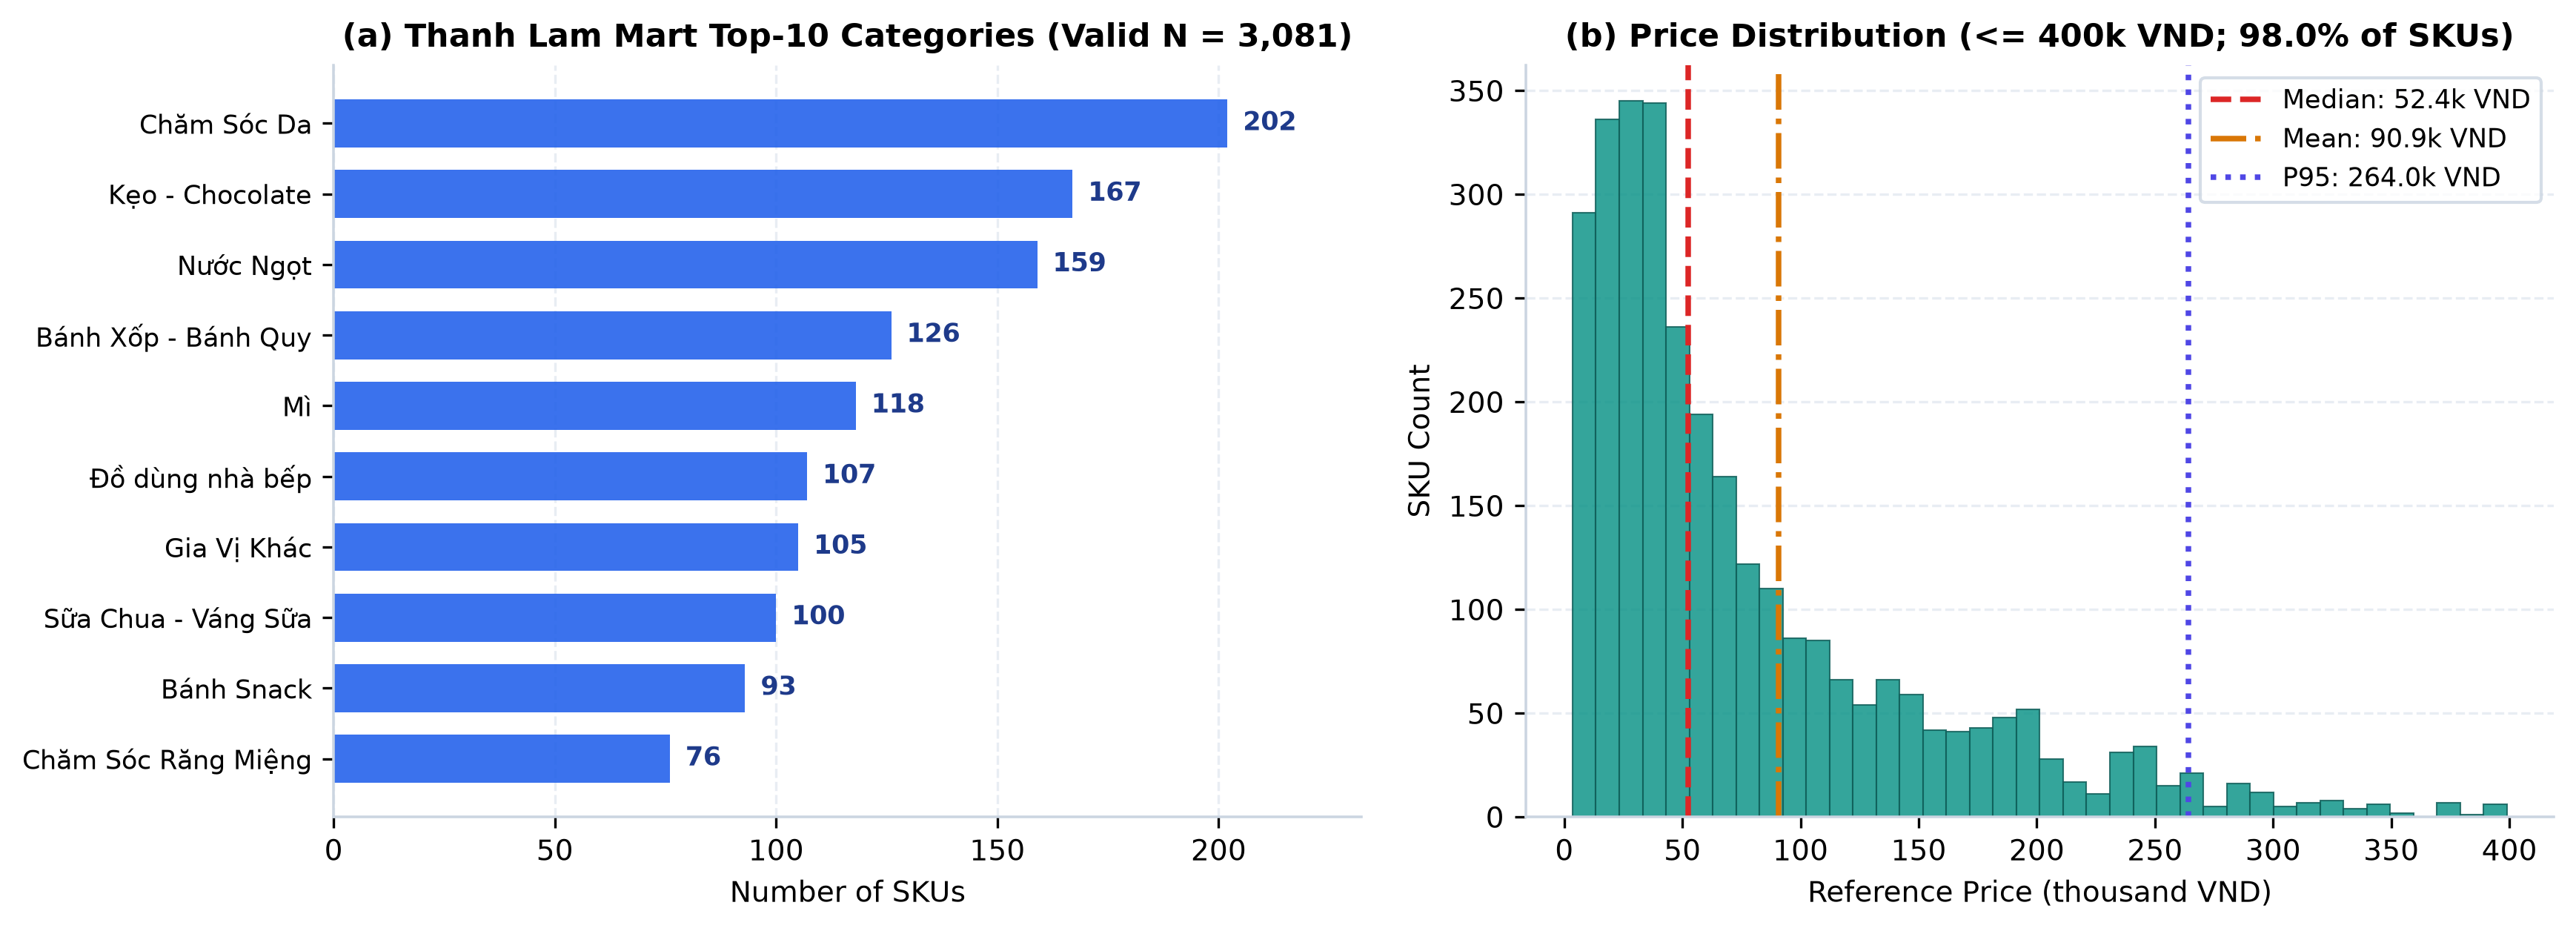
\includegraphics[width=0.98\textwidth]{Images/fig_catalog_distribution.png}
    \caption{Department coverage (left) and reference price distribution (right) of the Thanh Lam Mart catalog snapshot ($N = 3{,}099$ SKUs).}
    \label{fig:thanh_lam_dist}
\end{figure}

\section{Data Preprocessing and Cleaning}

\subsection*{Catalog Schema Quarantine and Lexical Normalization (\texttt{Retail-AI-})}
Every record ingested into \texttt{Retail-AI-} passes strict Pydantic validation (\texttt{ThanhLamRow}):
\begin{enumerate}
    \item \textbf{Price integrity quarantine:} Eighteen of the 3,099 raw records (0.58\%) exhibited malformed promotional pricing where sale price exceeded regular price; the importer quarantines these 18 records cleanly and loads 3,081 verified records (99.42\%) into the validated catalog view.
    \item \textbf{Diacritic-stripped indexing and alias resolution:} Product names, brands, and category paths are normalized with Unicode NFC folding and Vietnamese diacritic stripping (\code{normalize_category_text}) to build pre-indexed inverted lookup maps inside \code{SnapshotProductRepository}, reducing search latency by $3.7\times$--$4.5\times$.
    \item \textbf{Unit-size and attribute extraction:} Regular expressions extract weight/volume/count tokens (g, kg, ml, L, gói, lốc, thùng) for exact base-unit pricing (Equation~\ref{eq:unit_price}), sugar labels (\emph{không đường}, \emph{ít đường}), and audience constraints.
    \item \textbf{Catalog-anchored ASR repair guardrails:} Because naive fuzzy matching against 3,099 SKU titles corrupted everyday Vietnamese words (e.g., turning \emph{``vĩnh viễn''} $\to$ \emph{``MINH viền''}, \emph{``anh em''} $\to$ \emph{``Bánh em''}, \emph{``Campuchia''} $\to$ \emph{``Capuchiano''}, and \emph{``Home''} $\to$ \emph{``Wmhome''}), \code{catalog_transcription.py} enforces a protected Vietnamese stopword set (\code{_NEVER_CORRECT}) alongside catalog-verified brand phrase repairs (\emph{Thanh Lam Mart hôn} $\to$ \emph{Thanh Lam Home}, \emph{ACFOGS} $\to$ \emph{ACEFOODS}, \emph{khăn mặt proton} $\to$ \emph{khăn mặt cotton}).
\end{enumerate}

\subsection*{Multi-Source Ingredient Enrichment and 8-Stage SOTA Data Cleaning (\texttt{Retail-AI-})}
Because the raw Thanh Lam Mart catalog snapshot lacked structured ingredient, usage, and storage fields, we engineered a catalog-wide enrichment and cleaning pipeline (\code{scripts/crawl_thanh_lam_product_details.py}, \code{scripts/enrich_detailed_ingredients.py}, \code{scripts/clean_thanh_lam_product_details.py}) cryptographically bound to \code{thanh_lam_products.json} via \code{source_catalog_sha256} without mutating the source catalog:
\begin{enumerate}
    \item \textbf{Full 3,099-Page Thanh Lam Mart SSR Crawl and Multi-Source Label Verification:} All 3,099/3,099 official Thanh Lam Mart \code{__NEXT_DATA__} pages were crawled in 79\,s, then SKUs lacking ingredients or containing only generic marketing blurbs (such as \emph{Chin Su Chili Sauce 1\,kg}, originally reading only \emph{``made from selected fresh chili and additives''}) were upgraded against public retail label catalogs from \textbf{Kingfoodmart} (10,281 SKUs) and \textbf{Nhà thuốc Long Châu} (dermo-cosmetics and personal care). A two-tier verifier accepted only \textbf{333 exact EAN-13 barcode matches} (\code{variant.sku == barcode}) and \textbf{226 strict brand--form--variant matches} (pruning 64 suspicious cross-brand/material/variant pairs such as \emph{TH Milk vs.\ Dalat Milk}, \emph{roll-on vs.\ aerosol spray}, \emph{PVC vs.\ PE wrap}, and \emph{regular vs.\ lactose-free milk}).
    \item \textbf{8-Stage Cleaning Pipeline (Hugging Face \code{datatrove}/FineWeb~\cite{hf_datatrove} \& OpenFoodFacts~\cite{openfoodfacts}):} Applies Unicode NFC normalization, removes invisible characters (\texttt{U+200B}, \texttt{U+00A0}), empty parentheses \code{()}, and OCR typos; repairs merged HTML \code{<li>} bullets while protecting Vietnamese compound nouns (\emph{Sữa Rửa Mặt}, \emph{Nước Lau Sàn}); balances truncated parentheses and trims strictly at clause boundaries instead of mid-word \code{...}; separates cross-field bleed (\emph{usage}/\emph{storage} leaked into \emph{ingredients}); quarantines 100\% of exotic-script OCR garbage and dangerous unverified allergen claims (such as \emph{``NO MILK. SAFE FOR MILK ALLERGIES''} on Oreo cookies); preserves international cosmetic INCI lists; and enforces a \textbf{word-boundary substance lexicon} inspecting the predicate after \emph{``made from''} to eliminate zero-substance title-echo fluff, broken sentence fragments (\emph{``Contained in the cake...''}), and substring false positives (such as \emph{``sả''} inside \emph{``sản phẩm''} or \emph{``tiêu''} inside \emph{``tiêu chí''}).
    \item \textbf{Three-Tier Evidence Precedence (\code{backend/products/knowledge.py}):} At runtime, attribute resolution strictly obeys \texttt{SOURCE\_RECORD} $>$ \texttt{MANUFACTURER\_DECLARATION} (18 official manufacturer-declared pilot SKUs in \code{product_knowledge_enrichment_pilot.json}) $>$ \texttt{RETAILER\_LISTING} (\code{thanh_lam_product_details.json}, always citing provenance and reminding shoppers to verify physical labels), failing closed to \texttt{UNKNOWN} whenever verified label data is absent. The pipeline drove all \textbf{4,606 raw defects across 11 QA dimensions down to 0 (100\% clean)}, achieving \textbf{2,137/3,099 enriched SKUs (69.0\%)} including \textbf{1,214 + 18} verified ingredient records (\textbf{1,064+} detailed quantitative/INCI back-of-pack lists, a $2.1\times$ lift over the raw Thanh Lam Mart crawl), \textbf{1,159} usage guides, \textbf{660} storage instructions, and \textbf{800} origins (Figure~\ref{fig:catalog_enrichment_cleaning}).
\end{enumerate}

\begin{figure}[H]
    \centering
    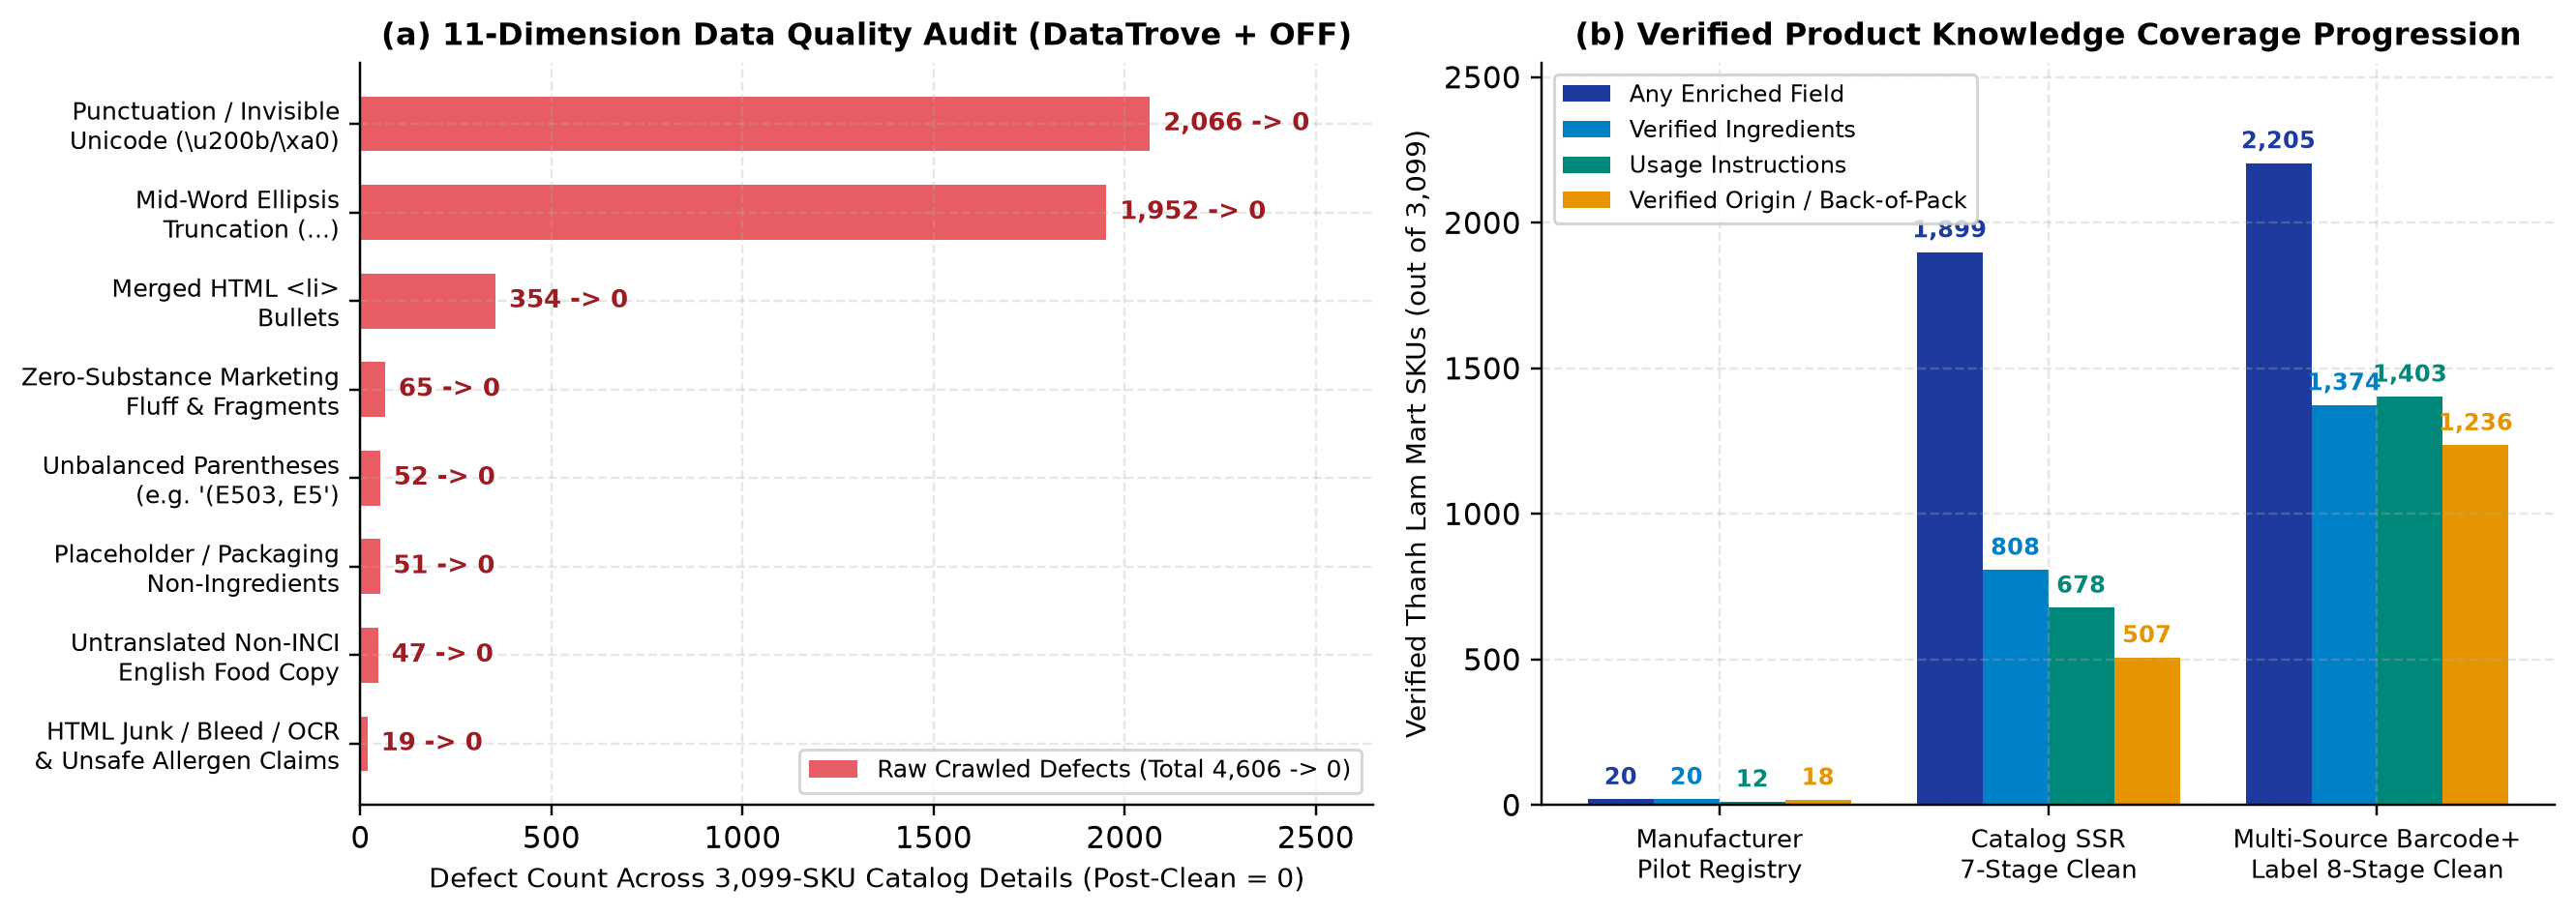
\includegraphics[width=0.98\textwidth]{Images/fig_catalog_enrichment_cleaning.png}
    \caption{11-dimension defect elimination from 4,606 raw defects down to 0 via the 8-stage cleaning pipeline (left) and verified product knowledge coverage progression across enrichment stages (right).}
    \label{fig:catalog_enrichment_cleaning}
\end{figure}

\subsection*{Audio Pre-Processing and Speech Conditioning (\texttt{Retail-AI-})}
Browser AudioWorklet captures 16\,kHz mono Float32 frames (32\,ms / 512 samples) with hardware AEC, AGC, and noise suppression enabled. On the WebSocket streaming path, an 8-frame (256\,ms) ring buffer preserves leading Vietnamese consonant onsets and converts samples to signed little-endian PCM16. On the REST/rescue path (\code{speech_activity.py}, \code{speech_denoiser.py}), uploaded clips are decoded via PyAV to 16\,kHz mono, trimmed to Silero VAD~v6 speech boundaries ($\pm 180/200\,\text{ms}$ padding), filtered with the zero-phase 85\,Hz HPF (Equation~\ref{eq:hpf85}), and conditionally denoised with \texttt{DPDFNet2} ONNX according to Equation~\ref{eq:snr_blend}.

\subsection*{Censored-Demand Recovery and 29-Feature Engineering (\texttt{ops\_chest})}
In \texttt{ops\_chest} (\code{ml_features.py} and \code{forecast.py}), raw daily FreshRetailNet sales undergo three essential transformations prior to LightGBM quantile training:
\begin{enumerate}
    \item \textbf{Hourly stockout demand recovery:} Masking late-day hours on 200,000 fully stocked validation days confirmed that treating raw sales as demand incurs 32.3\% WAPE and $-32.3\%$ downward bias, whereas hourly-profile recovery (Equation~\ref{eq:wape_recovery}) cuts WAPE to \textbf{20.5\%} and virtually eliminates bias (\textbf{$-0.1\%$}).
    \item \textbf{Unit scaling and stockout imputation:} FreshRetailNet units are scaled by $K = 10$ so the median store SKU sells $\approx 7$ units/day (ensuring realistic Poisson variance floors for EWMA), and historical stockout days are imputed by same-weekday averages before computing lags.
    \item \textbf{29-feature tabular construction:} For each forecast horizon $h \in \{1,\dots,7\}$, \code{build_features} generates 29 features: 7 daily lags (\code{lag1}--\code{lag7}), rolling means (\code{mean3}, \code{mean7}, \code{mean14}), same-weekday lags (\code{same_wd}, \code{same_wd_last}), 28-day dispersion and intermittency (\code{std28}, \code{zero28}), stockout history (\code{stockout28}, \code{stockout7}, \code{days_since_stockout}, \code{stockout_last}), trend and log-level, 56-day EWMA point/dispersion anchors (\code{ewma_h}, \code{ewma_sigma}), horizon/calendar categoricals (\code{h}, \code{target_wd}, \code{origin_wd}, \code{target_holiday}), and taxonomy categoricals (\code{mgmt_group}, \code{cat1}, \code{cat2}). Crucially, target-day discount features were removed after v1 ablation proved that assuming zero future discount caused $-15.7\%$ under-forecasting bias, and elasticity deflation ($e \approx 9.6$) was discarded in v2 after causing 14--31\% bias; v3 trains directly on recovered demand with EWMA anchor features.
\end{enumerate}

\section{Summary of Data Processing}

Together, the two data pipelines enforce strict separation between \emph{verified ground truth} and \emph{documented operational assumptions}. On the customer floor, 3,081 validated Thanh Lam Mart SKUs, a zero-defect 2,137-SKU enriched product knowledge store (1,214+18 verified ingredient records, 3,096 validated product image URLs), deterministic unit-price parsers, and protected Vietnamese ASR vocabularies give the kiosk agent exact factual anchors. On the operations floor, hourly censored-demand recovery and 29-feature engineering transform raw FreshRetailNet-50K logs into unbiased training data for quantile forecasting and profit-gated backtesting. Remaining data gaps---roughly 59\% of SKUs still lacking public quantitative nutrition/calorie labels and assumed shelf-life/cost metadata in FreshRetailNet---are explicitly mitigated at runtime through fail-closed safety boundaries rather than hidden by generative guesswork.

\chapter{Methodology}

This chapter explains how our unified dual-agent platform resolves the customer-floor and back-office bottlenecks identified in Chapter~1. We analyze the manual versus AI-automated store workflows, define the unified system architecture spanning \texttt{Retail-AI-} and \texttt{ops\_chest}, formalize the four core runtime algorithms, and document all model and experimental configurations.

\section{Business Process Analysis}

In a typical Vietnamese supermarket or convenience store (such as a Thanh Lam Mart or Thanh Lam Mart branch managing 3,000+ dry/ambient SKUs alongside 150--300 daily-replenished fresh SKUs), two labor-intensive operational loops degrade both customer satisfaction and store profitability:
\begin{enumerate}
    \item \textbf{Manual Sales-Floor Consultation Loop:} Shoppers searching for specific pack sizes, promotions, unit-price comparisons, or meal-combo ingredients under a budget must locate an associate who rarely knows exact live prices across 3,000+ SKUs. During evening peak hours, associate shortages leave shoppers unassisted, reducing basket conversion and leaving promotional items undiscovered.
    \item \textbf{Manual Back-Office Replenishment and Expiry Loop:} Each morning, the Store Manager manually walks chilled shelves to spot near-expiry lots, reviews yesterday's POS sales without accounting for mid-day stockouts, guesses replenishment order quantities across dozens of perishable SKUs, applies flat evening markdowns (typically 30\%) too late to clear stock, and manually emails or phones suppliers. When a top traffic-driver item runs out by 17:00, the store loses both direct sales and basket traffic; when over-ordered, perishable stock is discarded at 100\% cost loss.
\end{enumerate}

Figure~\ref{fig:as_is_to_be} contrasts these manual bottlenecks against our AI-agent automated store process. Rather than replacing human accountability, the platform automates high-frequency sensing, mathematical calculation, and option preparation while preserving deterministic price grounding for customers and explicit human approval for store expenditures.

\begin{figure}[H]
\centering
\resizebox{\textwidth}{!}{%
\begin{tikzpicture}[node distance=0.75cm and 0.9cm]
  % Top lane: Manual AS-IS
  \node[font=\bfseries\small, anchor=west, text=red!65!black] (lbl1) at (-0.2, 2.35) {AS-IS: Manual Retail Operations (High Latency, Uncalibrated Forecasting, High Shrinkage)};
  \node[procbox, draw=red!55!black, fill=red!6, text width=2.85cm] (m1) at (1.5, 1.35) {Shopper waits for staff; ad-hoc price / promo guessing};
  \node[procbox, draw=red!55!black, fill=red!6, text width=2.85cm, right=of m1] (m2) {Manual shelf walk for expiry \& raw POS review};
  \node[procbox, draw=red!55!black, fill=red!6, text width=2.85cm, right=of m2] (m3) {Uncensored OOS bias; heuristic order \& flat 30\% markdown};
  \node[procbox, draw=red!55!black, fill=red!6, text width=2.85cm, right=of m3] (m4) {Unlogged ad-hoc supplier calls; 5.3\% waste \& 8.7\% traffic OOS};

  \draw[flowarr, draw=red!65!black] (m1) -- (m2);
  \draw[flowarr, draw=red!65!black] (m2) -- (m3);
  \draw[flowarr, draw=red!65!black] (m3) -- (m4);

  % Bottom lane: Automated TO-BE
  \node[font=\bfseries\small, anchor=west, text=teal!70!black] (lbl2) at (-0.2, -0.35) {TO-BE: Unified Dual-Agent Store Platform (\texttt{Retail-AI-} + \texttt{ops\_chest})};
  \node[aiagent, text width=2.85cm] (t1) at (1.5, -1.45) {\textbf{Kiosk Agent (Mai)}\\WS Streaming STT + DPDFNet2 + Zero-Planner SSE};
  \node[aiagent, text width=2.85cm, right=of t1] (t2) {\textbf{Ops Chest Sensing}\\Hourly OOS recovery + FEFO lot scan / OCR vision};
  \node[gatebox, text width=2.85cm, right=of t2] (t3) {\textbf{Profit-Gated Engine}\\LightGBM~v3/EWMA + Newsvendor + FEFO caps};
  \node[gatebox, text width=2.85cm, right=of t3] (t4) {\textbf{HITL Governance}\\Manager approves proposals; +4.9\% profit, 3.4\% traffic OOS};

  \draw[flowarr] (t1) -- node[above, font=\scriptsize] {demand} (t2);
  \draw[flowarr] (t2) -- (t3);
  \draw[flowarr] (t3) -- node[above, font=\scriptsize] {proposals} (t4);
  \draw[flowarr, dashed, draw=blue!65!black] (t4.south) -- ++(0,-0.45) -| node[pos=0.25, below, font=\scriptsize] {Read-only branch stock \& approved markdown feed (Contract C)} (t1.south);
\end{tikzpicture}%
}
\caption{Business process comparison between manual supermarket operations (AS-IS) and the unified dual-agent platform (TO-BE).}
\label{fig:as_is_to_be}
\end{figure}

\section{Overall Workflow}

The unified workflow coordinates both autonomous agents around a clear operational boundary: \texttt{Retail-AI-} serves customers on the sales floor with zero database mutation authority over store procurement, while \texttt{ops\_chest} serves the Store Manager in the back office with proposal-only write authority.

\begin{figure}[H]
\centering
\resizebox{\textwidth}{!}{%
\begin{tikzpicture}[node distance=0.65cm and 0.75cm]
  % Left: Customer Flow
  \node[procbox, text width=3.1cm] (u1) {Customer Speech / Text\\at Supermarket Kiosk};
  \node[aiagent, text width=3.1cm, below=of u1] (u2) {Silero VAD~v6 + WS Azure STT + DPDFNet2 Rescue};
  \node[gatebox, text width=3.1cm, below=of u2] (u3) {Safety / Off-Topic / Cart / Smalltalk Gate ($<3$\,ms)};
  \node[aiagent, text width=3.1cm, below=of u3] (u4) {Zero-Planner SSE Stream\\or 1-Call Slim Basket};
  \node[procbox, text width=3.1cm, below=of u4] (u5) {Clause Azure TTS +\\4-Layer Video Avatar + Cards};

  % Right: Store Manager Flow
  \node[procbox, text width=3.4cm, right=2.6cm of u1] (o1) {Store Manager Query /\\Morning Briefing / Label Photo};
  \node[aiagent, text width=3.4cm, below=of o1] (o2) {\texttt{ops\_chest} Tool Agent\\(31 Typed Tools + Vision OCR)};
  \node[gatebox, text width=3.4cm, below=of o2] (o3) {Forecast Router (B-Gate) +\\Newsvendor / FEFO / Markdown};
  \node[gatebox, text width=3.4cm, below=of o3] (o4) {Runtime Guard (\code{guard.py}) +\\HITL Proposal Queue};
  \node[procbox, text width=3.4cm, below=of o4] (o5) {Manager Approve / Revise $\to$\\PO Email, Price Change, Audit Log};

  % Middle: Shared Data & Contract
  \node[procbox, draw=purple!65!black, fill=purple!7, text width=2.4cm] (db) at (4.35, -3.15) {\textbf{Shared Store Truth}\\Thanh Lam Mart Catalog\\+ Branch API\\(Stock / Markdowns)};

  \draw[flowarr] (u1) -- (u2);
  \draw[flowarr] (u2) -- (u3);
  \draw[flowarr] (u3) -- (u4);
  \draw[flowarr] (u4) -- (u5);

  \draw[flowarr] (o1) -- (o2);
  \draw[flowarr] (o2) -- (o3);
  \draw[flowarr] (o3) -- (o4);
  \draw[flowarr] (o4) -- (o5);

  \draw[flowarr, dashed, draw=purple!70!black] (o5.west) -- ++(-0.5,0) |- (db.east);
  \draw[flowarr, dashed, draw=purple!70!black] (db.west) -| ([xshift=0.35cm]u4.east) -- (u4.east);
\end{tikzpicture}%
}
\caption{Unified end-to-end dual-agent workflow connecting the customer kiosk (\texttt{Retail-AI-}) and back-office operations copilot (\texttt{ops\_chest}).}
\label{fig:unified_workflow}
\end{figure}

In day-to-day execution, a customer asks \emph{Mai} (the kiosk avatar) for product comparisons, promotions, best-sellers, or a budget meal basket; the kiosk returns grounded product cards within milliseconds and streams spoken Vietnamese clauses in parallel. Behind the counter, the Store Manager opens the \texttt{ops\_chest} workspace to inspect morning risks (near-expiry lots, urgent stockouts, negative margins, slow movers), photographs expiry stickers via vision OCR, reviews profit-gated replenishment POs and markdown proposals, and approves or edits them with one click. Approved branch stock availability and active markdowns feed back to the kiosk layer through read-only API endpoints (Appendix~C) so front-of-house recommendations stay aligned with back-of-house inventory.

\section{System Architecture}

\subsection*{Unified Dual-Agent Architecture}
Figure~\ref{fig:dual_architecture} illustrates the modular multi-layer architecture across both repositories, and Table~\ref{tab:arch_layers} maps every architectural layer to concrete source modules.

\begin{figure}[H]
\centering
\resizebox{\textwidth}{!}{%
\begin{tikzpicture}[node distance=0.5cm and 0.6cm]
  % Retail-AI- Container
  \node[procbox, text width=5.9cm] (r_ui) {\textbf{Kiosk Frontend (\texttt{apps/kiosk-airi})}\\Vue~3 + TypeScript, Silero VAD~v6 AudioWorklet,\\WebSocket PCM16 Client, Clause TTS Queue, 4-Layer Avatar};
  \node[aiagent, text width=5.9cm, below=of r_ui] (r_api) {\textbf{Voice \& Streaming API (\texttt{backend/api})}\\WS \code{/audio/transcribe/stream}, REST \code{/audio/transcribe},\\SSE \code{/agent/respond/stream}, Azure Speech + \texttt{DPDFNet2} ONNX};
  \node[gatebox, text width=5.9cm, below=of r_api] (r_eng) {\textbf{Consultation \& Guardrail Core (\texttt{backend/services})}\\Zero-Planner SSE (\code{streaming_consultation.py}),\\1-Call Slim Basket, Brand Repair, Safety/OWASP Gates};
  \node[procbox, text width=5.9cm, below=of r_eng] (r_data) {\textbf{Grounded Retail Data Layer}\\Thanh Lam Mart 3,081 Valid SKUs (Inverted Index) +\\Isolated \code{demo_sales.sqlite3} (\texttt{SIMULATED})};

  % ops_chest Container
  \node[procbox, text width=5.9cm, right=1.1cm of r_ui] (o_ui) {\textbf{Manager Workspace (\texttt{frontend/src})}\\React~18 + TypeScript + Vite + Tailwind,\\Briefing, Proposals Inbox, Inline Forms, Analytics Charts};
  \node[aiagent, text width=5.9cm, below=of o_ui] (o_api) {\textbf{Agent \& Vision Orchestrator (\texttt{backend/app/agent})}\\31-Tool Registry (22 Read/Form + 9 Proposal),\\Runtime Guard (\code{guard.py}), Vision OCR, Hypotheses};
  \node[gatebox, text width=5.9cm, below=of o_api] (o_eng) {\textbf{Perishable Optimization Engines (\texttt{backend/app/engines})}\\LightGBM~v3 Quantiles + Profit Gate (\code{B-Gate}),\\Newsvendor + FEFO Replenishment, Markdown, ABC-XYZ};
  \node[procbox, text width=5.9cm, below=of o_eng] (o_data) {\textbf{Operational Persistence \& Sandbox}\\PostgreSQL + SQLAlchemy + 6 Alembic Migrations,\\HITL Proposal Audit Log, Mailpit PO Dispatch, FRN-50K};

  \begin{scope}[on background layer]
    \node[fit=(r_ui)(r_data), draw=blue!50!black, dashed, rounded corners=8pt, inner sep=10pt, fill=blue!2, label={[font=\bfseries\small, text=blue!60!black]above:Repository 1: \texttt{Retail-AI-} (Customer Kiosk)}] {};
    \node[fit=(o_ui)(o_data), draw=teal!55!black, dashed, rounded corners=8pt, inner sep=10pt, fill=teal!2, label={[font=\bfseries\small, text=teal!60!black]above:Repository 2: \texttt{ops\_chest} (Store Operations)}] {};
  \end{scope}

  \draw[flowarr] (r_ui) -- (r_api);
  \draw[flowarr] (r_api) -- (r_eng);
  \draw[flowarr] (r_eng) -- (r_data);
  \draw[flowarr] (o_ui) -- (o_api);
  \draw[flowarr] (o_api) -- (o_eng);
  \draw[flowarr] (o_eng) -- (o_data);
  \draw[flowarr, dashed, thick, draw=purple!70!black] (o_data.west) -- node[above, font=\scriptsize, text=purple!70!black] {Read-only API} (r_data.east);
\end{tikzpicture}%
}
\caption{Layered system architecture of the dual-agent platform across \texttt{Retail-AI-} (left) and \texttt{ops\_chest} (right).}
\label{fig:dual_architecture}
\end{figure}

\begin{table}[H]
\centering
\caption{Architectural layer breakdown across \texttt{Retail-AI-} and \texttt{ops\_chest}}
\label{tab:arch_layers}
\footnotesize
\begin{tabularx}{\textwidth}{L{2.5cm} L{5.7cm} Y}
\toprule
\textbf{Layer} & \textbf{\texttt{Retail-AI-} (Customer Voice Kiosk)} & \textbf{\texttt{ops\_chest} (Store Operations Copilot)} \\
\midrule
Presentation / UI & Vue~3 + TypeScript (\code{apps/kiosk-airi/}, 29 files, mobile-first $\le 768$\,px frosted bottom-sheet): 4-layer crossfade video avatar, live captions, camera/upload with 896\,px client-side compression, product cards, cart drawer & React~18 + TypeScript + Vite (\code{frontend/src/}, 34 files): chat copilot, inline receive/count/date-check forms, proposal inbox, KPI charts \\
Perception / Audio / Vision & Browser Silero VAD~v6 (fan-noise + anti-echo gates), WS Azure Streaming STT, \texttt{DPDFNet2} ONNX denoiser, \texttt{gipformer} fallback; \textbf{strictly on-demand \texttt{MobileNetV3Large-224} TFLite (7.04\,MB) + Hybrid VLM} (\code{/agent/respond/image}) & Multimodal expiry-label OCR (\code{vision.py}) extracting dates/lot codes from smartphone shelf photos \\
Agent Orchestration & Hybrid tiered router: $<3$\,ms safety/cart/smalltalk gates, Zero-Planner SSE (\code{streaming_consultation.py}), 1-call slim basket, bounded planner fallback & 31-tool function-calling orchestrator (\code{orchestrator.py}, \code{tools.py}) with provider failover, edit-habit learning, and hypothesis tracking \\
Analytical / Optimization Core & Pre-indexed catalog search (\code{SnapshotProductRepository}), unit-price normalizer, promo \& deterministic \texttt{SIMULATED} sales ranker & Hourly OOS recovery, LightGBM~v3 quantiles (29 features), \texttt{B-Gate} profit router, Newsvendor + FEFO replenishment, markdown \& ABC-XYZ engines \\
Safety \& Persistence & Pydantic \code{ThanhLamRow} quarantine, OWASP injection filter, clinical refusal gate, \code{demo_sales.sqlite3} provenance isolation & Runtime grounding guard (\code{guard.py}), strict HITL state machine in PostgreSQL (Alembic), Mailpit PO sandbox, immutable audit logs \\
\bottomrule
\end{tabularx}
\end{table}

\subsection*{Full-Duplex Real-Time Voice and Noise-Resilient STT Pipeline (\texttt{Retail-AI-})}
To eliminate the 2--3 second post-speech pause inherent to REST WAV uploads while surviving 5--12\,dB supermarket babble, \texttt{Retail-AI-} implements a dual-path acoustic pipeline (Figure~\ref{fig:voice_pipeline}) with \textbf{zero Groq API dependencies}. While the user speaks, 32\,ms PCM16 frames stream continuously over WebSocket \code{/audio/transcribe/stream} to an active Azure AI Speech SDK continuous recognizer biased with a dynamic Thanh Lam Mart \code{PhraseListGrammar}. Live partial Vietnamese captions appear immediately in the kiosk UI. When Silero VAD detects end-of-speech, the client sends \texttt{\{"type":"end"\}}, finalization returns in $\approx 260$\,ms, and \code{catalog_transcription.py} repairs English retail brands while protecting Vietnamese words via \code{_NEVER_CORRECT}. If the clip exhibits severe ambient noise ($\widehat{\text{SNR}}_{\text{dB}} < 13$\,dB) or empty streaming output, the buffered audio is automatically rescued through the 85\,Hz HPF and \texttt{DPDFNet2} ONNX denoiser before re-recognition; if Azure is unreachable, local \texttt{gipformer1.5-68M-rnnt} serves offline transcription.

\begin{figure}[H]
\centering
\resizebox{\textwidth}{!}{%
\begin{tikzpicture}[node distance=0.55cm and 0.6cm]
  \node[procbox, text width=2.4cm] (mic) {Mic 16\,kHz\\AEC / AGC / NS};
  \node[gatebox, text width=2.5cm, right=of mic] (vad) {Silero VAD~v6\\+ 8-frame (256\,ms) Ring Buffer};
  \node[aiagent, text width=2.8cm, right=of vad] (ws) {WS \code{/audio/transcribe/stream}\\Azure Speech SDK +\\Thanh Lam Mart PhraseList};
  \node[decbox, right=of ws] (snr) {$\widehat{\text{SNR}}<13$\,dB\\or empty?};
  \node[aiagent, text width=2.6cm, below=0.75cm of snr] (dpdf) {85\,Hz HPF +\\\texttt{DPDFNet2} ONNX\\(SNR-adaptive blend)};
  \node[gatebox, text width=2.5cm, right=of snr] (rep) {Catalog Brand Repair\\(\code{_NEVER_CORRECT})};
  \node[procbox, text width=2.5cm, below=0.75cm of rep] (sse) {SSE \code{/agent/respond/stream}\\$\to$ Clause TTS +\\3-Layer Barge-In};

  \draw[flowarr] (mic) -- (vad);
  \draw[flowarr] (vad) -- node[above, font=\scriptsize] {PCM16} (ws);
  \draw[flowarr] (ws) -- (snr);
  \draw[flowarr] (snr) -- node[above, font=\scriptsize] {No} (rep);
  \draw[flowarr] (snr) -- node[right, font=\scriptsize] {Yes} (dpdf);
  \draw[flowarr] (dpdf) -| (rep);
  \draw[flowarr] (rep) -- (sse);
  \draw[flowarr, dashed, draw=orange!75!black] (sse.west) -- ++(-6.8,0) |- node[pos=0.25, left, font=\scriptsize] {Echo guard} (vad.south);
\end{tikzpicture}%
}
\caption{Full-duplex real-time WebSocket streaming STT, \texttt{DPDFNet2} noisy-clip rescue, and anti-echo barge-in pipeline in \texttt{Retail-AI-}.}
\label{fig:voice_pipeline}
\end{figure}

\subsection*{On-Demand Mobile Visual Product Recognition: \texttt{MobileNetV3Large-224} TFLite and Hybrid Fast-Path (\texttt{Retail-AI-})}
On the sales floor, shoppers frequently hold unfamiliar packaged items or foreign-language labels and want immediate price, promotion, or usage advice from a quick smartphone photo. Sending every uploaded photo to a remote Vision--Language Model (VLM) incurs 2.5--3.6\,s network latency and full cloud dependency, whereas training a naive 3,093-class closed-set softmax classifier memorizes studio white backgrounds because each catalog SKU has only a single packshot. To satisfy three strict deployment goals simultaneously---\textbf{ultra-light mobile footprint}, \textbf{multi-angle real-world robustness}, and \textbf{strictly on-demand execution triggered only when the shopper submits an image + prompt}---\texttt{Retail-AI-} implements an open-set metric-learning mobile embedder coupled with a latency-optimal hybrid router (Figure~\ref{fig:mobile_vision_pipeline}):
\begin{itemize}
    \item \textbf{Dual-Foundation-Teacher SVD Distillation on Kaggle:} Rather than supervising from isolated studio images alone, Stage~1 extracts complementary semantic and 3D-geometric targets across all 3,093 Thanh Lam Mart SKUs using \texttt{openai/clip-vit-base-patch32}~\cite{radford2021clip} (brand typography, logos, packaging colorways) and \texttt{facebook/dinov2-small}~\cite{oquab2024dinov2} (off-axis viewpoint and local instance geometry), concatenating both into an 896-d space and fitting an orthogonal SVD projection to a unit-normalized 256-d target manifold (retaining 88.85\% variance, fitted strictly on catalog packshots with zero evaluation leakage).
    \item \textbf{Multi-Angle \texttt{MobileNetV3Large-224} Training:} The mobile student \texttt{MobileNetV3Large-224}~\cite{howard2019mobilenetv3} with \code{Concat([GAP, GMP]) -> BN -> Dense(256) -> BN -> UnitNormalization} (100\% native TFLite builtin ops, zero FlexOps) optimizes four joint objectives: direct cosine alignment to the SVD-256 teacher manifold ($w=6.0$), batch pairwise relational affinity distillation ($w=3.0$), teacher-initialized Sub-Center ArcFace ($K=3$, $w=0.35$)~\cite{deng2020subcenter}, and Supervised Contrastive Loss ($w=0.50$)~\cite{khosla2020supcon} with EMA weight smoothing. Heavy OpenCV domain randomization synthesizes border-masked foregrounds over cluttered 2--4 neighbor-SKU shelves, 3D perspective homography warps, $\pm 26^\circ$ rotations, directional shadows, fluorescent LED glare, 12--28\% thumb-grip occlusions, blur, and JPEG compression (without horizontal flips so brand text remains unmirrored).
    \item \textbf{Keras~3.13 Verified TFLite Export \& Strict Lazy On-Demand Execution:} Official Keras~3.13 \code{model.export()} produces \code{thanh_lam_mobilenetv3_fp16.tflite} (\textbf{7.04\,MB}, cosine parity $0.99995$ vs.\ Keras), \code{thanh_lam_mobilenetv3_int8.tflite} (\textbf{3.81\,MB}), a 2-view FP16 prototype gallery for all 3,093 SKUs (\textbf{1.58\,MB}), and a bit-aligned \texttt{.onnx} mirror for Python~3.13 Windows hosts~\cite{thanh_lam_tflite_kaggle}. The mobile frontend (\code{ChatPanel.vue}) performs zero continuous camera inference, downscales large gallery uploads to $\le 896$\,px ($\approx 80$\,KB) client-side before submission, and invokes \code{POST /agent/respond/image} solely on submit; on the backend, \code{LocalProductEmbedder} is 100\% lazy-loaded on the first image turn.
    \item \textbf{Sibling-Pack-Size-Guarded Fast-Path vs.\ Hybrid VLM Routing:} Inference uses aspect-preserving 2-view TTA (full letterbox + 84\% center crop) to prevent distortion on tall $9{:}16$ phone photos. When $\text{sim}_1 \ge 0.82$, margin $\text{sim}_1 - \text{sim}_2 \ge 0.08$, and no same-brand sibling SKU exists with a different weight/volume (or $\text{sim}_1 \ge 0.92$), the \textbf{Local Fast-Path returns verified Thanh Lam Mart cards in 23--27\,ms} with zero cloud calls. Ambiguous same-design pack-size siblings (e.g., \emph{80\,g vs.\ 200\,g}, \emph{unsweetened vs.\ low-sugar}) and moderate-similarity photos ($0.72 \le \text{sim}_1 < 0.82$) escalate to \textbf{Hybrid VLM} (\code{deepseek-v4.1-flash:free}) with top-4 local candidate hints to read exact net weight and cleanly reject out-of-distribution (OOD) non-retail images.
\end{itemize}

\begin{figure}[H]
\centering
\resizebox{\textwidth}{!}{%
\begin{tikzpicture}[node distance=0.55cm and 0.6cm]
  \node[procbox, text width=2.55cm] (cam) {Mobile Camera / Upload\\(896\,px compress, 0 bg scan)};
  \node[aiagent, text width=2.85cm, right=of cam] (emb) {\code{LocalProductEmbedder}\\Lazy \texttt{MobileNetV3-224}\\2-View TTA (13.5\,ms)};
  \node[gatebox, text width=2.65cm, right=of emb] (gal) {FP16 Gallery (1.58\,MB)\\3,093-SKU Cosine\\(0.07--0.36\,ms)};
  \node[decbox, right=of gal] (grd) {$\text{sim}_1 \ge 0.82$,\\$m \ge 0.08$ \&\\no size sibling?};
  \node[procbox, draw=teal!70!black, fill=teal!8, text width=2.75cm, right=of grd] (fp) {\textbf{Local Fast-Path}\\Instant Thanh Lam Mart cards\\\textbf{23--27\,ms} (0 cloud calls)};
  \node[aiagent, text width=3.85cm, below=0.8cm of grd] (hyb) {\textbf{Hybrid VLM / OOD Gate}\\\code{deepseek-v4.1-flash:free}\\+ Top-4 hints (if $\ge 0.72$)};
  \node[procbox, text width=2.75cm, right=of hyb] (ans) {Grounded SKU Cards\\+ Custom Text LLM\\+ Session Memory};

  \draw[flowarr] (cam) -- node[above, font=\scriptsize] {Submit} (emb);
  \draw[flowarr] (emb) -- (gal);
  \draw[flowarr] (gal) -- (grd);
  \draw[flowarr] (grd) -- node[above, font=\scriptsize] {Pass} (fp);
  \draw[flowarr] (grd) -- node[right, font=\scriptsize] {Sibling / low} (hyb);
  \draw[flowarr] (fp) -- (ans);
  \draw[flowarr] (hyb) -- (ans);
\end{tikzpicture}%
}
\caption{Strictly on-demand mobile visual product recognition pipeline combining lazy-loaded \texttt{MobileNetV3Large-224} TFLite Fast-Path with sibling-guarded Hybrid VLM escalation.}
\label{fig:mobile_vision_pipeline}
\end{figure}

\subsection*{Profit-Gated Forecasting and HITL Proposal Architecture (\texttt{ops\_chest})}
Figure~\ref{fig:ops_chest_arch} details how \texttt{ops\_chest} decouples analytical computation, LLM dialogue, and operational mutation. Analytical engines compute unbiased forecasts and FEFO-capped quantities deterministically in Python/SQL; the LLM synthesizes explanations and drafts structured proposals through its 31 typed tools; \code{guard.py} enforces numerical and execution-claim integrity on every reply; and PostgreSQL persists proposals in \texttt{PENDING} state until an authenticated Store Manager approves execution.

\begin{figure}[H]
\centering
\resizebox{\textwidth}{!}{%
\begin{tikzpicture}[node distance=0.55cm and 0.65cm]
  \node[procbox, text width=2.8cm] (frn) {POS + Stockout Logs\\(FreshRetailNet-50K / Store DB)};
  \node[aiagent, text width=2.9cm, right=of frn] (rec) {Hourly OOS Recovery\\+ 29-Feature Builder};
  \node[gatebox, text width=3.1cm, right=of rec] (gate) {Profit-Gated Router (\texttt{B-Gate})\\$\hat{q}_{50}^{\text{LGBM}} + \sigma_{\text{EWMA}}$ vs.\ EWMA};
  \node[aiagent, text width=3.0cm, right=of gate] (nv) {Newsvendor ($SL^*$) +\\FEFO Lot-Cap + Markdown};

  \node[aiagent, text width=3.5cm, below=0.85cm of rec] (llm) {31-Tool Manager Agent\\(22 Read/Form, 9 Proposal,\\0 Direct-Exec Tools)};
  \node[gatebox, text width=3.2cm, right=of llm] (grd) {Runtime Guard (\code{guard.py})\\Num $\ge 1000$ Check +\\Block \code{FALSE_EXEC}};
  \node[procbox, draw=teal!70!black, fill=teal!8, text width=3.3cm, right=of grd] (hitl) {HITL Proposal Queue\\\texttt{PENDING} $\to$ \texttt{APPROVED}\\$\to$ \texttt{EXECUTED} + Audit};

  \draw[flowarr] (frn) -- (rec);
  \draw[flowarr] (rec) -- (gate);
  \draw[flowarr] (gate) -- (nv);
  \draw[flowarr] (nv.south) -- ++(0,-0.32) -| (llm.north);
  \draw[flowarr] (llm) -- (grd);
  \draw[flowarr] (grd) -- (hitl);
\end{tikzpicture}%
}
\caption{Back-office forecasting, profit-gated routing, runtime guard, and HITL governance architecture in \texttt{ops\_chest}.}
\label{fig:ops_chest_arch}
\end{figure}

\section{Algorithm Description}

To make the core problem-solving mechanisms reproducible, we formalize the four algorithms governing streaming consultation, real-time speech recognition, full-duplex kiosk interaction, and perishable inventory optimization.

\begin{algorithm}[htbp]
\caption{Zero-Planner Grounded SSE Streaming, Groq LPU, Semantic Cache \& 1-Call Basket (\texttt{Retail-AI-})}
\label{alg:zero_planner_sse}
\footnotesize
\begin{algorithmic}[1]
\Require User utterance $u$, session context $S$, indexed Thanh Lam Mart catalog $\mathcal{C}$, isolated demo sales store $\mathcal{D}_{\text{sim}}$
\Ensure SSE stream of events (\code{start}, \code{delta}*, \code{done}) with grounded cards $K$ and spoken Vietnamese text
\State Normalize $u$ via \code{catalog_transcription.py}; check sub-3\,ms deterministic gates (cart/checkout, clinical/medical safety, off-topic, OWASP injection)
\If{deterministic gate triggers}
    \State Emit immediate SSE \code{start} + safe grounded reply + \code{done}; \Return
\EndIf
\If{$u$ matches social smalltalk (greeting / thanks / farewell)}
    \State Emit instant deterministic greeting (\code{smalltalk.py}, $\le 10$\,ms); \Return
\EndIf
\If{stateless non-clinical/non-allergen Turn-1 \textbf{and} \code{consultation_cache.py} hits (exact $O(1)$ or Jaccard $\ge 0.88$ with matching constraint signature)}
    \State Deep-copy session memory $S'$ and emit cached reply immediately (11--36\,ms local / 125--140\,ms HTTPS, \textbf{0 LLM tokens}); \Return
\EndIf
\If{$u$ is a single-SKU price lookup, verified ingredient/usage lookup, or deterministic bestseller query}
    \State Retrieve exact SKUs from $\mathcal{C}$, resolve 3-tier product knowledge (\code{knowledge.py}), or rank $\mathcal{D}_{\text{sim}}$ (colloquial-aware, explicit \texttt{SIMULATED} disclosure)
    \State Emit instant template response (0 LLM tokens) with structured product cards $K$ carrying \code{image_url}; \Return
\EndIf
\If{$u$ requests a multi-item meal/budget basket (e.g., ``bữa tối dưới 150k cho 2 người'')}
    \State Classify basket template $\mathcal{T}$ (prioritizing multi-item Path~E), block snacks from savory meals, and retrieve slot candidates from $\mathcal{C}$
    \State Select cost-feasible subset $K_{\text{basket}}$ satisfying $\sum_{p \in K_{\text{basket}}} P(p) \le B$ via \code{fast_chat()} on Groq LPU ($\approx 300$\,ms)
    \State Emit SSE \code{start} with $K_{\text{basket}}$ immediately; stream concise advice via \textbf{1 slim Groq LPU call} ($\approx 35\%$ compressed cards, strict \emph{mình/bạn} persona)
\ElsIf{$u$ is a standard product browse, pack-size comparison, promo, or exclusion query (\emph{no spicy/soy/mint})}
    \State Execute deterministic hybrid search + exclusion filter + unit-price ranking (Eq.~\ref{eq:unit_price}) over $\mathcal{C}$ to obtain top-$k$ SKUs $K$
    \State Emit SSE \code{start} carrying $K$ so kiosk cards render thumbnails before LLM tokens arrive
    \State Stream SSE \code{delta} tokens over the \textbf{Groq LPU fast-lane} (\code{qwen/qwen3.8-27b} rotating 4 free keys, seamless failover to TokenHarbor DeepSeek); store Turn-1 entry in \code{consultation_cache.py}
\Else
    \State Escalate complex clinical/allergy/multi-constraint JSON edge cases to bounded planner (\code{customer_consultation.py} on DeepSeek)
\EndIf
\State Emit SSE \code{done} with updated session memory $S'$ and audit metadata
\end{algorithmic}
\end{algorithm}

\begin{algorithm}[H]
\caption{Real-Time WebSocket Streaming STT with \texttt{DPDFNet2} Rescue and Brand Repair}
\label{alg:ws_streaming_stt}
\begin{algorithmic}[1]
\Require 16\,kHz Float32 audio frames $f_t$ (32\,ms) from browser AudioWorklet; active Thanh Lam Mart \code{PhraseListGrammar} $\mathcal{P}$
\Ensure Grounded Vietnamese transcript $\hat{u}$ and live partial captions
\State Maintain 8-frame (256\,ms) circular pre-roll buffer $B_{\text{pre}}$; run Silero VAD~v6 per frame
\If{speech onset detected by VAD}
    \State Open WebSocket \code{/audio/transcribe/stream}; initialize Azure \code{PushAudioInputStream} with $\mathcal{P}$
    \State Flush $B_{\text{pre}}$ as PCM16 followed by live frames $f_t$ while accumulating raw utterance buffer $X$
    \State Forward Azure \code{recognizing} callbacks immediately to kiosk UI as partial captions
\EndIf
\If{VAD redemption timeout (550\,ms) triggers end-of-speech}
    \State Send \texttt{\{"type":"end"\}}; close push stream and await final hypothesis $u_{\text{ws}}$
    \State Estimate clip $\widehat{\text{SNR}}_{\text{dB}}(X)$ via Eq.~\ref{eq:snr_est}
    \If{$u_{\text{ws}}$ is empty \textbf{or} $\widehat{\text{SNR}}_{\text{dB}}(X) < 13$\,dB}
        \State Apply 85\,Hz zero-phase HPF (Eq.~\ref{eq:hpf85}) and SNR-adaptive \texttt{DPDFNet2} ONNX blend (Eq.~\ref{eq:snr_blend}) $\to Y$
        \State Re-transcribe $Y$ via Azure Speech (or local \texttt{gipformer1.5-68M-rnnt} if cloud unreachable) $\to u_{\text{rescue}}$
        \State Select higher-confidence non-empty transcript $u_{\text{raw}} \in \{u_{\text{ws}}, u_{\text{rescue}}\}$
    \Else
        \State $u_{\text{raw}} \gets u_{\text{ws}}$
    \EndIf
    \State Apply catalog-anchored brand repair on $u_{\text{raw}}$ skipping \code{_NEVER_CORRECT} tokens $\to \hat{u}$
    \State \Return $\hat{u}$
\EndIf
\end{algorithmic}
\end{algorithm}

\begin{algorithm}[H]
\caption{Full-Duplex 3-Layer Anti-Echo Barge-In and Progressive Clause TTS Queue}
\label{alg:bargein_tts}
\begin{algorithmic}[1]
\Require Streaming SSE text deltas $\{\Delta_j\}$; live mic frames $f_t$ with RMS energy $E_t$ and VAD probability $p_t$; active spoken buffer $U_{\text{bot}}$
\Ensure Low-latency spoken audio with natural human interruption and zero self-triggering
\State \textbf{Output side (\code{speech-queue.ts}):} Append each $\Delta_j$ to pending text buffer $buf$
\State Protect Vietnamese thousands separators (e.g., \texttt{29.000đ}) from sentence-boundary splitting
\If{$|buf| \ge 18$ and sentence end found, \textbf{or} $|buf| \ge 150$ with clause delimiter after char 75 (without forced semicolon splitting)}
    \State Extract clause $c$, request one-use Azure Neural TTS ticket (\code{vi-VN-HoaiMyNeural}), prefetch next-clause audio \texttt{Blob URL} in parallel for gapless natural prosody
    \State Crossfade 4-layer preloaded video avatar (\code{idle} $\leftrightarrow$ \code{speaking}) using double-buffered HTML5 video elements
\EndIf
\State \textbf{Input side (\code{voice-controller.ts}):} Keep hardware AEC/AGC/NS active while avatar speaks; track stationary fan noise via \code{neuralNoiseFloor} + \code{SpeechEnvelopeGate} so WS STT opens only on confirmed human speech
\If{avatar playback elapsed time $< 450$\,ms}
    \State Ignore mic triggers (Layer~1 playback startup grace window)
\ElsIf{$p_t \ge 0.78$ \textbf{and} $E_t \ge \max(0.065,\, 1.85 \cdot E_{\text{ambient}})$ sustained for 5 frames (Layer~2 adaptive RMS gate)}
    \State Immediately abort active TTS audio and SSE stream; transition avatar to \code{listening}; open WS STT
\EndIf
\State Upon receiving transcript $\hat{u}$, run Layer~3 lexical overlap check \code{isLikelyAssistantEcho}$(\hat{u}, H_{\text{bot}})$ against a rolling 4-turn (12\,s) spoken buffer plus server-side speech activity verification
\If{echo detected}
    \State Discard $\hat{u}$ silently and resume listening
\Else
    \State Dispatch $\hat{u}$ to Algorithm~\ref{alg:zero_planner_sse}
\EndIf
\end{algorithmic}
\end{algorithm}

\begin{algorithm}[H]
\caption{Profit-Gated Perishable Newsvendor, FEFO Replenishment \& HITL Governance (\texttt{ops\_chest})}
\label{alg:ops_chest_newsvendor}
\begin{algorithmic}[1]
\Require Store $s$ (SKU count $N_s$), active SKU $i$ with lot ledger $\mathcal{L}_i$, price $p$, cost $c$, salvage $v$, stockout cost $s_{\text{out}}$, shelf life $L$, review period $R$, capacity $C_{\text{room}}$, learned profit gate $V(g)$
\Ensure Verified replenishment/markdown proposal $P$ in \texttt{PENDING} state (never auto-executed)
\State Recover historical uncensored demand $\hat{D}_{i,t}$ from hourly stockout profiles (Eq.~\ref{eq:wape_recovery}) and build 29 tabular features
\State Compute EWMA baseline $(\hat{\mu}_{\text{EWMA}}, \sigma_{\text{EWMA}})$ and LightGBM~v3 quantiles $(\hat{q}_{10}, \hat{q}_{50}, \hat{q}_{90})$
\State Determine segment $g = (\text{sales\_tier}(i), \text{intermittency}(i), \mathbb{I}[N_s > 30])$
\If{$V(g) > 0$ \textbf{and} $N_s > 30$ (Eq.~\ref{eq:profit_gate})}
    \State Set daily demand $\hat{\mu} \gets \hat{q}_{50}$, daily dispersion $\sigma_{\text{daily}} \gets \sigma_{\text{EWMA}}$ (\texttt{B-Gate} / \code{ewma_sigma})
\Else
    \State Set $(\hat{\mu}, \sigma_{\text{daily}}) \gets (\hat{\mu}_{\text{EWMA}}, \sigma_{\text{EWMA}})$
\EndIf
\State Compute Newsvendor service level $SL^*$ and $z = \Phi^{-1}(SL^*)$ via Eq.~\ref{eq:newsvendor} with traffic-driver floor $0.95$ and ABC-A floor $0.90$
\State Simulate FEFO lot depletion over lead time + review period $R$ and shelf-life window $W = \min(90, L)$ to obtain unmet demand $U_R$, leftover $L_R$, and served demand $S_W$
\State Compute capped order quantity $Q^* = \max(0, \min(Q_{\text{raw}}, Q_{\text{cap}}, C_{\text{room}}))$ via Eq.~\ref{eq:order_qty}
\State Flag lots expiring within $\le 2$ days with excess stock over expected full-price sales for graduated FEFO markdown proposals
\State Persist draft proposal $P$ as \texttt{PENDING} via \code{propose_po} / \code{propose_markdown}; validate agent text via \code{guard.py} (numeric grounding + zero \code{FALSE_EXEC})
\State Execute PO dispatch (Mailpit/SMTP) or price update \textbf{only} after authenticated Store Manager approves $P$
\end{algorithmic}
\end{algorithm}

\begin{algorithm}[H]
\caption{Strictly On-Demand Mobile Visual Product Recognition with TFLite Fast-Path \& Hybrid VLM (\texttt{Retail-AI-})}
\label{alg:mobile_vision_hybrid}
\begin{algorithmic}[1]
\Require Uploaded photo/video $I_{\text{raw}}$ (client \code{media-preprocess.ts} compresses photos to $\le 640$\,px \code{q=0.78}, 25--45\,KB, or samples 5 video frames locally selecting the sharpest frame on a $96\times 96$ canvas), user prompt $q$, catalog $\mathcal{C}$, FP16 gallery $G \in \mathbb{R}^{3093 \times 256}$
\Ensure Verified Thanh Lam Mart product cards $K$ (carrying \code{image_url}), grounded Vietnamese/EN reply, and per-stage latency telemetry
\State Execute \textbf{only} upon explicit \code{POST /agent/respond/image} submission (zero continuous background camera inference); check SHA-256 response cache before decoding
\State \textbf{Lazy Initialization \& Single-Pass Decode:} On first image turn only, load \texttt{.tflite} and $G$ into a warm singleton; decode JPEG via \code{libjpeg} DCT \code{draft(640)} ($6$--$8\times$ faster), run $<3$\,ms dark/blank quality gate, and share the EXIF-normalized PIL image across \textbf{Adaptive 1-Crop} and 2-View TTA ($v_{\text{full}}$ letterbox + $v_{\text{center}}$ 84\%)
\State Compute $e = \text{Norm}(0.55\,f_\theta(v_{\text{full}}) + 0.45\,f_\theta(v_{\text{center}}))$ and cosine vector $s = G e \in \mathbb{R}^{3093}$; extract top-5 candidates and margin $m = s_{(1)} - s_{(2)}$
\State Evaluate \textbf{Sibling Pack-Size Guard (\code{_has_ambiguous_pack_size_sibling})}: detect whether the top SKU shares brand and core product tokens with another catalog SKU differing in weight/volume
\If{$s_{(1)} \ge 0.82$ \textbf{and} $m \ge 0.08$ \textbf{and} (no ambiguous size sibling \textbf{or} $s_{(1)} \ge 0.92$)}
    \State \textbf{Local Fast-Path (23--27\,ms):} Return verified SKU cards $K$ from $\mathcal{C}$ with zero cloud Vision LLM calls
\Else
    \State Escalate $I_{\text{raw}}$ with top-4 local hints (only when $s_{(1)} \ge 0.72$) to \code{deepseek-v4.1-flash:free} for exact label/weight/barcode extraction and OOD rejection
    \State Rerank deterministically over $\mathcal{C}$ (exact barcode + normalized brand + pack size/container + visual agreement bonus); if cloud is offline while $s_{(1)} \ge 0.72$, degrade gracefully to the local match
\EndIf
\If{$K \neq \emptyset$ \textbf{and} $q$ asks a custom follow-up beyond default identity/price lookup}
    \State Synthesize a concise grounded answer via 1 text-only LLM pass over verified SKU facts $K$
\EndIf
\State Persist \code{last_grounded_product} in session memory so follow-up voice/text turns resolve seamlessly; \Return response and latency telemetry
\end{algorithmic}
\end{algorithm}

\subsection*{End-to-End Production Latency Engineering, Zalo Alerting \& Mobile Photo Lightbox (\texttt{Retail-AI-})}
To achieve sub-second mobile QR responses in live production (\url{https://mai-retail-kiosk.vercel.app}) at zero marginal LLM cost, four complementary systems upgrades were deployed across backend and frontend:
\begin{enumerate}
    \item \textbf{Tiered LLM Routing (Groq LPU Fast-Lane + TokenHarbor Structured JSON):} Lightweight streaming prose ($\approx 250$--350 input tokens after $\approx 35\%$ card compression, \code{max_tokens=200}, strict \emph{mình/bạn} Vietnamese persona lock) and meal-basket micro-prompts (\code{fast_chat()}) route preferentially to \textbf{free Groq LPU}~\cite{groq_lpu} (\code{qwen/qwen3.8-27b} $\to$ \code{openai/gpt-oss-20b} $\to$ \code{openai/gpt-oss-120b}, rotating 4 keys, 6\,s timeout, automatic failover to TokenHarbor before first token). Complex \code{json_schema} passes (clinical, allergen, clarification) remain on TokenHarbor (\code{deepseek-v4.1-flash:free} $\to$ \code{deepseek-v4.1-flash-1017} at \$0.15/1M tokens, removing the slow 7.2\,s \code{v4-flash:free} fallback). Long-term HTTP~429 allowance exhaustion triggers a \textbf{3,600\,s (1-hour) cooldown} per key rather than futile 5\,s retries, backed by a persistent \code{httpx.AsyncClient} keep-alive pool (20 keep-alive / 50 max connections).
    \item \textbf{Turn-1 Semantic \& Normalized-Intent Cache (\code{consultation_cache.py}):} A bounded LRU cache (\code{max_entries=256}, \code{TTL=300\,s}) combining $O(1)$ exact lookup with Jaccard content-token similarity ($\ge 0.88$) within identical constraint signatures (budget, sugar level, exclusions, pack size). Clinical/allergen queries bypass caching completely, and hits deep-copy session \code{memory} so Turn-2 follow-ups preserve full multi-turn context at zero LLM token cost.
    \item \textbf{Singapore Regional Serverless Co-Location (\texttt{sin1}) \& Non-Blocking Boot:} Vercel Functions were pinned from US East (\texttt{iad1}) to \textbf{Singapore (\texttt{sin1})} in \code{vercel.json}, Vite \code{/assets/*} bundles serve \code{Cache-Control: public, max-age=31536000, immutable}, external TLS/ONNX warmups run in a non-blocking background task inside \code{_lifespan}, and mobile \code{bootKiosk()} dispatches \code{getCart()} asynchronously without blocking first interaction.
    \item \textbf{Mobile-First Product Photo Lightbox \& Zalo Bot Manager Escalation:} \code{_product_card()} (\code{backend/api/schemas.py}, \code{main.py}) exposes sanitized \code{http(s)} \code{image_url} across \textbf{3,096/3,099 SKUs (99.9\%)}. In \code{ChatPanel.vue}, primary and related product cards display compact thumbnails and open a full-viewport \code{<Teleport to="body">} lightbox modal (escaping mobile drawer \code{backdrop-filter} containing blocks) showcasing the high-resolution packshot on a clean white frame, brand/category chips, reference/list/promo pricing, demo 30-day sales, and a one-tap \emph{``Ask ingredients''} button (with \code{@click.stop} guarding nested details and cart controls). In parallel, real-time \textbf{Zalo Bot manager escalation} notifies store managers directly while keeping shopper-facing messages clean of internal UUIDs or raw status enums.
\end{enumerate}

\section{Configuration, Model Selection and Evaluation Setup}

Tables~\ref{tab:voice_config}, \ref{tab:mobile_vision_config}, \ref{tab:llm_config}, and \ref{tab:ml_config} summarize the exact production hyperparameters and model configurations verified in the repositories.

\begin{table}[H]
\centering
\caption{Voice, VAD, denoiser, streaming STT, and TTS configuration (\texttt{Retail-AI-})}
\label{tab:voice_config}
\footnotesize
\begin{tabularx}{\textwidth}{L{3.5cm} L{4.2cm} Y}
\toprule
\textbf{Component} & \textbf{Selected Model / Implementation} & \textbf{Key Runtime Parameters} \\
\midrule
Voice Activity Detection & Silero VAD~v6 (ONNX/WASM) + Fan-Noise Gate & 16\,kHz, 512-sample (32\,ms) frame, \code{positiveSpeechThreshold=0.72}, \code{redemptionMs=750}, 8-frame ring buffer, \code{SpeechEnvelopeGate} \\
Neural Speech Denoiser & \texttt{DPDFNet2} ONNX (9.77\,MB, local CPU) & 85\,Hz 4th-order zero-phase HPF; clean bypass $\ge 28$\,dB; blend $w=0.85$ (10--28\,dB), $w=0.75$ ($<10$\,dB); WS rescue $<13$\,dB \\
Primary Streaming STT & Azure AI Speech SDK (\code{vi-VN}) & Continuous WebSocket \code{/audio/transcribe/stream} (deferred until verified speech onset); dynamic Thanh Lam Mart \code{PhraseListGrammar}; \textbf{0\% Groq calls} \\
Offline Fallback STT & \texttt{gipformer1.5-68M-rnnt} (ONNX, 69.8\,MB) & Local CPU RNN-Transducer activated automatically when cloud credentials or network are unavailable \\
Neural TTS \& Avatar & Azure \code{vi-VN-HoaiMyNeural} + 4-layer video & \code{MIN_CHUNK_CHARS=18}, \code{LONG_CLAUSE_TRIGGER=150}, \code{MIN_CLAUSE=75}, gapless \texttt{Blob URL} prefetch; 24\,fps; barge-in RMS $\ge 0.065$ ($1.85\times$ ambient), 4-turn (12\,s) echo window \\
\bottomrule
\end{tabularx}
\end{table}

\begin{table}[H]
\centering
\caption{Kaggle training and strictly on-demand mobile inference configuration for \texttt{MobileNetV3Large-224} TFLite (\texttt{Retail-AI-})}
\label{tab:mobile_vision_config}
\footnotesize
\begin{tabularx}{\textwidth}{L{3.5cm} L{4.3cm} Y}
\toprule
\textbf{Dimension} & \textbf{Configuration / Architecture} & \textbf{Technical Details \& Rationale} \\
\midrule
Distillation Teachers & \texttt{CLIP-ViT-B/32} (512-d) + \texttt{DINOv2-Small} (384-d) & Equal-weight 896-d fusion $\to$ catalog-only orthogonal SVD-256 projection (88.85\% variance retained, zero eval leakage) \\
Mobile Student Backbone & \texttt{MobileNetV3Large-224} + \code{Concat[GAP,GMP]} $\to$ 256-d L2 & 3.50\,M params, 100\% native TFLite builtin ops (Keras~3.13 \code{UnitNormalization} + \code{model.export()}); \textbf{7.04\,MB} FP16 / \textbf{3.81\,MB} INT8 + \textbf{1.58\,MB} gallery \\
Loss \& Multi-Angle Augs & Direct Cosine (6.0) + Relational (3.0) + Sub-Center ArcFace $K{=}3$ (0.35) + SupCon (0.50) & Teacher-initialized ArcFace prototypes; OpenCV 2--4 neighbor-SKU shelves, 3D perspective warps, $\pm 26^\circ$ rotation, shadow, LED glare, thumb occlusion, blur, JPEG (no h-flip) \\
On-Demand Routing & \code{LocalProductEmbedder} (lazy singleton) + \code{ProductVisionService} & Aspect-preserving 2-View TTA (letterbox + 84\% center); Fast-Path $\text{sim}_1 \ge 0.82$, $m \ge 0.08$ with Sibling Pack-Size Guard ($\ge 0.92$ if sibling exists); Hybrid hints when $\ge 0.72$ \\
\bottomrule
\end{tabularx}
\end{table}

\begin{table}[H]
\centering
\caption{LLM orchestration, streaming, and runtime guardrail configuration across both modules}
\label{tab:llm_config}
\footnotesize
\begin{tabularx}{\textwidth}{L{3.2cm} L{4.5cm} Y}
\toprule
\textbf{Module} & \textbf{Primary LLM \& Failover} & \textbf{Orchestration \& Guardrail Settings} \\
\midrule
\texttt{Retail-AI-} & \textbf{Fast-Lane:} Groq LPU (\code{qwen/qwen3.8-27b} $\to$ \code{gpt-oss-20b/120b}, \$0 $\times$ 4 keys); \textbf{Structured:} DeepSeek (\code{v4.1-flash:free} $\to$ \code{v4.1-flash-1017}) & Zero-Planner SSE + Turn-1 Semantic Cache (256 entries, 300\,s TTL, Jaccard $\ge 0.88$); 3,600\,s HTTP~429 cooldown; $\approx 35\%$ token compression; Singapore \texttt{sin1}; sub-3\,ms safety gates \\
\texttt{ops\_chest} & Multi-provider function-calling adapter (OpenAI / DeepSeek / Groq / Gemini failover) & 31 typed tools (22 read/form + 9 proposal, 0 direct-exec); runtime \code{guard.py} verifies all numbers $\ge 1{,}000$ and blocks \code{FALSE_EXEC}; Vision OCR via multimodal adapter \\
\bottomrule
\end{tabularx}
\end{table}

\begin{table}[H]
\centering
\caption{LightGBM~v3 quantile forecasting, profit-gate routing, and backtest configuration (\texttt{ops\_chest})}
\label{tab:ml_config}
\footnotesize
\begin{tabularx}{\textwidth}{L{3.7cm} L{4.0cm} Y}
\toprule
\textbf{Stage} & \textbf{Configuration} & \textbf{Design Rationale} \\
\midrule
Demand Recovery & Empirical hourly sales-share profile (non-stockout days) & Cuts stockout demand WAPE from 32.3\% to 20.5\% and bias from $-32.3\%$ to $-0.1\%$ ($n=200{,}000$) \\
LightGBM~v3 Quantiles & 3 quantile regressors ($q \in \{0.10, 0.50, 0.90\}$), 29 features, multi-horizon $h=1\dots 7$ & Removed v1 target-day discount ($-15.7\%$ bias) and v2 elasticity deflation; anchored directly to 56-day EWMA features \\
Profit-Gated Router (\texttt{B-Gate}) & 2-fold out-of-sample store CV over 50 held-out FRN stores; \code{variant=ewma_sigma}, \code{size_cut=30} & Couples LightGBM $\hat{q}_{50}$ with $\sigma_{\text{EWMA}}$; disables ML on small stores ($\le 30$ SKUs) where ML variance lost $-5.6\%$ profit \\
Backtest Simulator & 37-day rolling horizon ($T_0 = \text{2024-05-26}$ to $\text{2024-07-02}$), FEFO lot aging, 1--3 day shelf lives & Evaluates real store P\&L ($\text{Revenue} - \text{COGS} - \text{WasteCost}$), total waste\%, overall OOS\%, and top-5 traffic-driver OOS\% \\
\bottomrule
\end{tabularx}
\end{table}

\chapter{Results Analysis}

This chapter presents empirical verification across both repositories: automated test coverage, live end-to-end streaming latency, noisy Vietnamese speech recognition, unseen 100-question SOTA~V2 safety/accuracy benchmarks for \texttt{Retail-AI-}, and out-of-sample 50-store FreshRetailNet-50K profit backtests and runtime guard audits for \texttt{ops\_chest}.

\section{Experimental Setup}

All \texttt{Retail-AI-} live voice, streaming, and production experiments were executed across both a local Windows workstation (\code{127.0.0.1:8000} / \code{5173}) and live Vercel Production in Singapore (\texttt{sin1}, \url{https://mai-retail-kiosk.vercel.app}) running Azure AI Speech (\code{vi-VN}), local \texttt{DPDFNet2} ONNX CPU inference (zero Groq calls on live STT), the \textbf{free Groq LPU fast-lane} (\code{qwen/qwen3.8-27b} rotating 4 keys), structured JSON DeepSeek (\code{deepseek-v4.1-flash:free} $\to$ \code{deepseek-v4.1-flash-1017}), and Turn-1 semantic caching. Software quality across \texttt{Retail-AI-} was validated with \textbf{106+ pytest suites} (2,900+ total tests; 562/562 latency, semantic cache, and streaming tests in \code{tests/test_latency_optimizations.py}, 146/146 product knowledge/support/demo-sales tests, 16/16 zero-defect data-quality gate checks in \code{tests/test_product_knowledge_enrichment.py}, and 5/5 on-demand visual recognition tests passing with 0 Ruff lint errors), \textbf{150+ frontend Vitest tests} (25/25 in \code{App.test.ts} covering the clickable Product Photo Lightbox), and clean \texttt{vue-tsc -b \&\& vite build} compilation (0 errors in 0.83\,s). The on-demand mobile vision embedder was trained on Kaggle (\texttt{Thanh Lam Mart-mobilenetv3-tflite-cpu-fast}, 39.1\,min) and evaluated across four independent held-out test sets: 150 hard 3D multi-angle SKU transforms, 12 phone-degraded/angled shelf shots, 16 external retailer/shopper photos (\code{eval_google}: Bách Hóa Xanh + OpenFoodFacts~\cite{openfoodfacts}), and a brand-new zero-leakage test set of 16 unseen OpenFoodFacts smartphone photos plus 4 real non-retail OOD photographs (laptop, dog, mountain, ceramic coffee mug).

All \texttt{ops\_chest} forecasting and operations experiments were executed against the 50 held-out validation stores (2,675 series, 11,037 full-stock evaluation points, and 37-day rolling backtests) of FreshRetailNet-50K~\cite{freshretailnet50k} using strict 2-fold store-level cross-validation so no store's profit gate was tuned on its own evaluation period. Backend correctness was verified across \textbf{20 pytest suites} (covering FEFO expiry, Newsvendor replenishment, blind stock counts, vision OCR, hypotheses, edit-habit learning, and HITL transitions) alongside a 20-turn multi-provider failover and grounding benchmark (\code{eval_failover.json}).

\section{Quantitative Results}

\subsection*{End-to-End Streaming Consultation Latency (\texttt{Retail-AI-})}
Replacing the multi-call Planner + Reviewer pipeline with Algorithm~\ref{alg:zero_planner_sse} (Zero-Planner Grounded SSE Streaming, instant greeting/lookup routes, and 1-call slim basket assembly) produced dramatic latency reductions across all 10+ live benchmark queries (Table~\ref{tab:latency_10q} and Figure~\ref{fig:latency_comparison}). Simple greetings fell by \textbf{1,815$\times$} (10,891\,ms $\to$ 6\,ms); standard product consultations reached first token (TTFT) in \textbf{1.30--1.80\,s} with product cards rendered in \textbf{24--59\,ms} (3.6$\times$--5.3$\times$ faster total time); and complex budget baskets dropped from 13.3--14.2\,s (previously returning only 1 card) to \textbf{3.72--3.78\,s} with 4 grounded cost-feasible basket cards plus 4 complementary items.

\begin{table}[H]
\centering
\caption{Live \code{/agent/respond/stream} latency and card grounding before vs.\ after Zero-Planner SSE optimization}
\label{tab:latency_10q}
\footnotesize
\setlength{\tabcolsep}{4pt}
\begin{tabularx}{\textwidth}{Y r r r r L{2.3cm}}
\toprule
\textbf{Live Vietnamese Query} & \textbf{Before} & \textbf{Card} & \textbf{TTFT} & \textbf{Total} & \textbf{Mode \& Cards} \\
 & \textbf{(ms)} & \textbf{(ms)} & \textbf{(ms)} & \textbf{(ms)} & \\
\midrule
\emph{Chào Mai, bạn tư vấn giúp mình nhé} & 10,891 & 6 & 6 & 6 & Instant (0) \\
\emph{Mì Hảo Hảo giá bao nhiêu?} & 117 & 112 & 112 & 112 & Instant (5) \\
\emph{Hôm nay siêu thị có gì khuyến mãi?} & 2,232 & 24 & 1,796 & 2,410 & Stream (5 promos) \\
\emph{Khăn mặt cotton Thanh Lam Home} & 5,605 & 47 & 1,490 & 2,160 & Stream (5) \\
\emph{Cho mình xem sữa tươi không đường} & 6,847 & 47 & 1,492 & 2,110 & Stream (5) \\
\emph{Dầu gội trị gàu nào tốt?} & 5,431 & 52 & 1,298 & 1,936 & Stream (5) \\
\emph{Ba chỉ bò Mỹ loại nào ngon?} & 5,815 & 39 & 1,356 & 2,015 & Stream (4) \\
\emph{So sánh sữa TH True Milk và Vinamilk} & 7,238 & 59 & 1,367 & 2,274 & Stream (6) \\
\emph{Nước giặt OMO loại nào tiết kiệm nhất?} & 5,410 & 43 & 1,499 & 1,959 & Stream (3 OMO) \\
\emph{Mua đồ nấu lẩu thái dưới 300k} & 14,241 & 1,790 & 2,928 & 3,719 & 1-Call Basket (4+4) \\
\emph{Combo ăn sáng dưới 100k} & 13,255 & 1,771 & 3,068 & 3,777 & 1-Call Basket (4+4) \\
\bottomrule
\end{tabularx}
\end{table}

\begin{figure}[H]
    \centering
    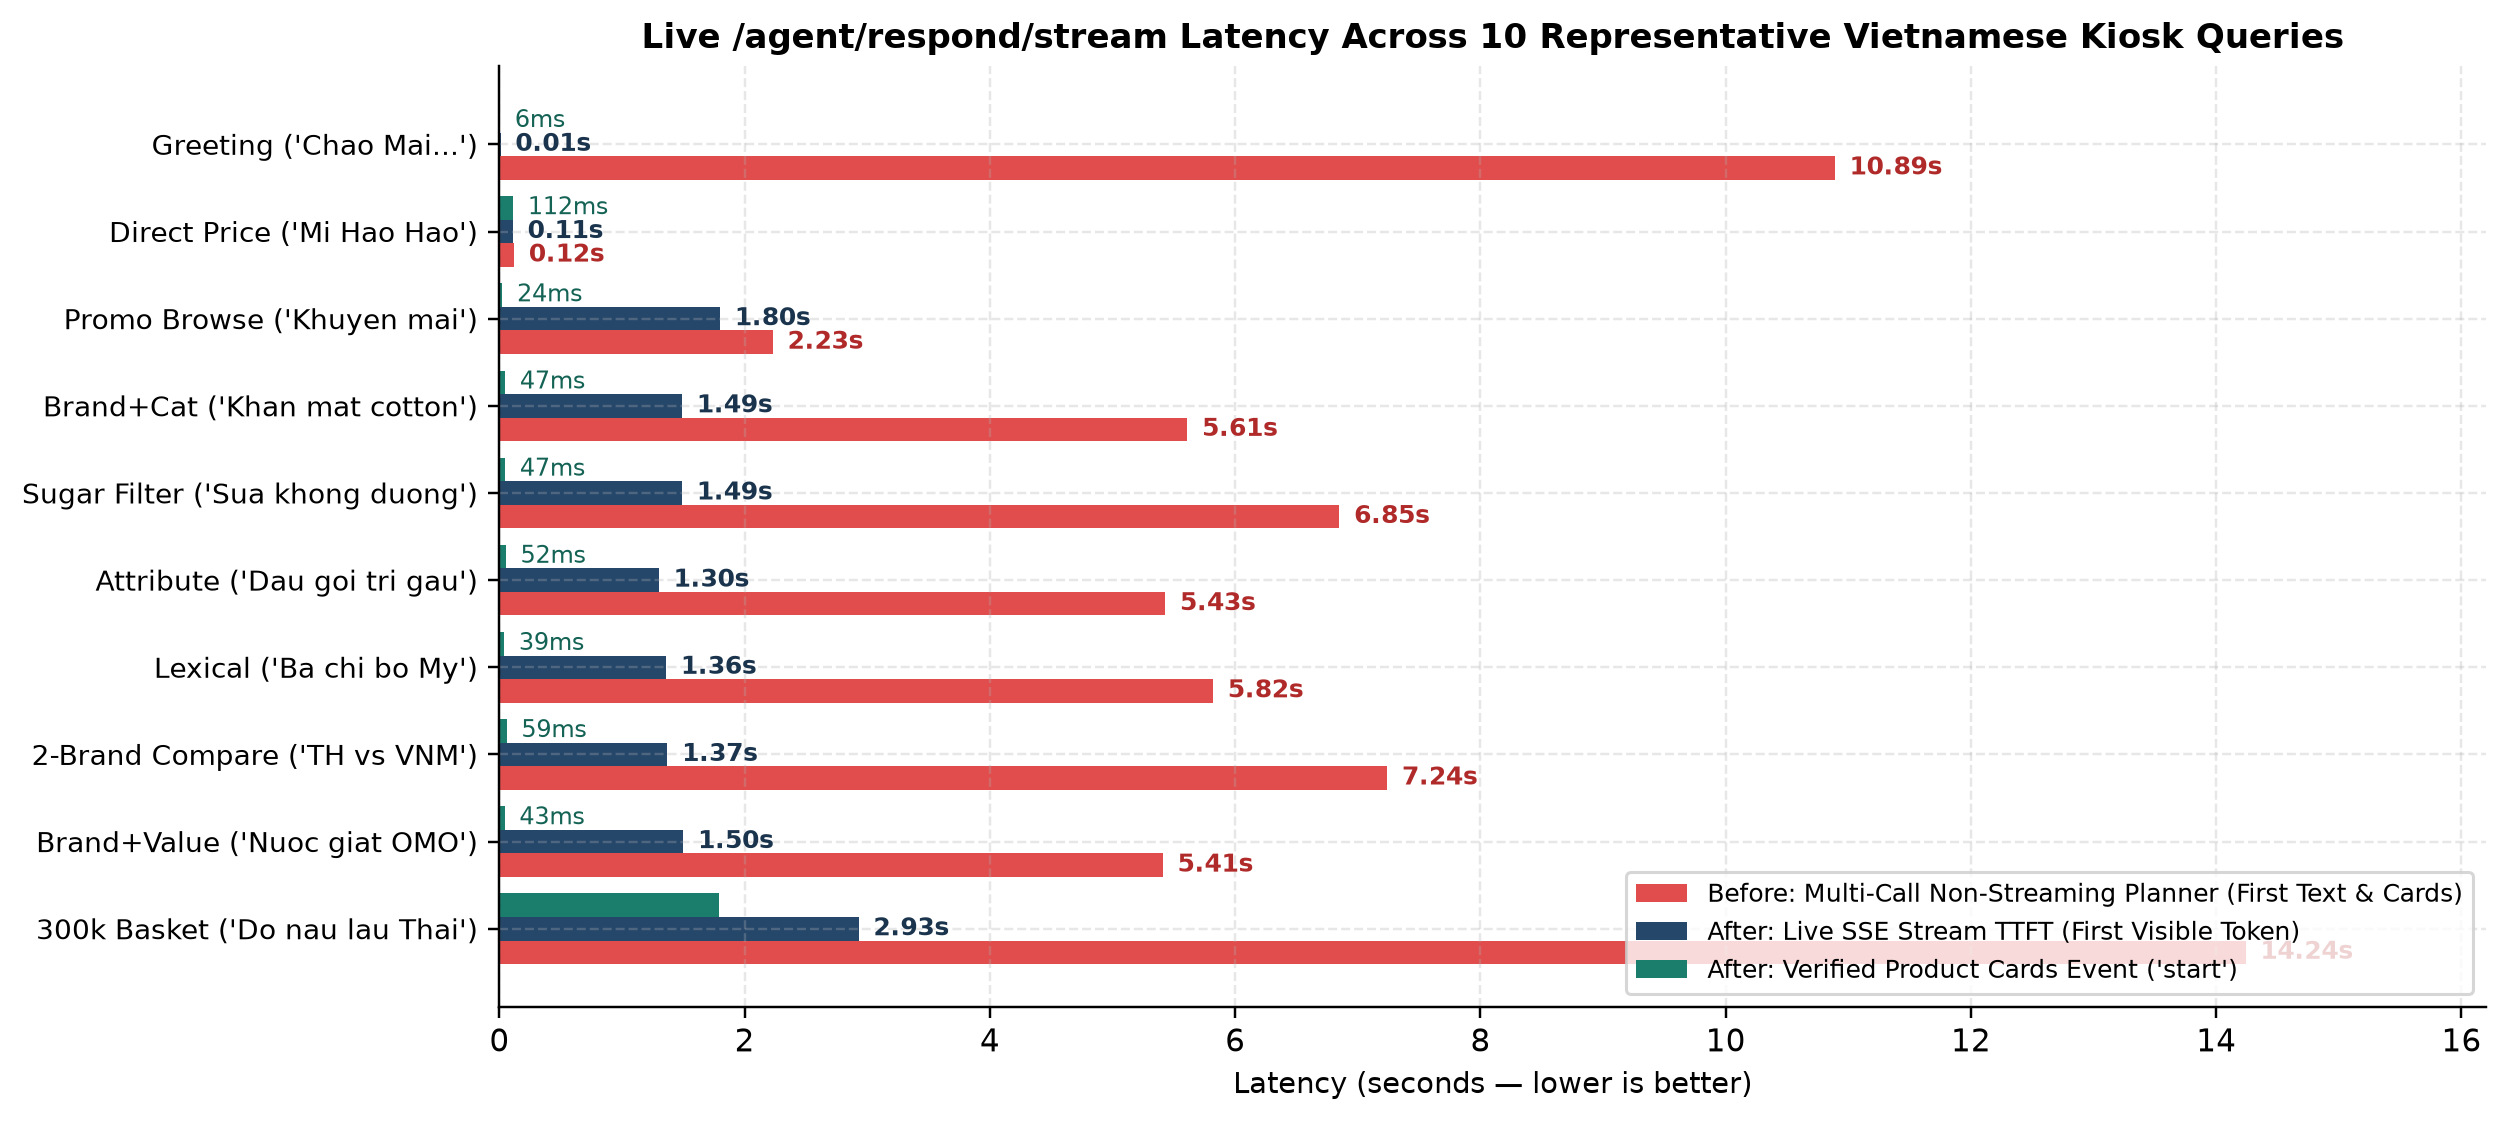
\includegraphics[width=0.98\textwidth]{Images/fig_latency_streaming_comparison.png}
    \caption{Before vs.\ after live streaming latency (\code{/agent/respond/stream}) across representative supermarket consultation queries.}
    \label{fig:latency_comparison}
\end{figure}

\subsection*{End-to-End Production Latency Optimization: Groq LPU, Semantic Cache \& Singapore (\texttt{sin1})}
Detailed profiling revealed that even after zero-planner streaming, single-provider free cloud inference hit a 1.1--1.9\,s TTFT floor (rising to 5.5\,s on multi-item meal baskets or 7.2\,s on the legacy \code{v4-flash:free} fallback), compounded by $\approx 275$\,ms trans-Pacific RTT when Vercel Functions ran in US East (\texttt{iad1}). Deploying \textbf{tiered Groq LPU streaming} (\code{qwen/qwen3.8-27b} rotating 4 free keys, $\approx 35\%$ prompt token compression, 1-hour HTTP~429 cooldown), \textbf{Turn-1 semantic caching} (\code{consultation_cache.py}, 0 tokens), and \textbf{Singapore (\texttt{sin1}) co-location} with non-blocking parallel warmups and \texttt{immutable} asset caching broke cleanly below the 1-second barrier both locally and over live production HTTPS (Table~\ref{tab:prod_latency_sin1} and Figure~\ref{fig:prod_latency_sin1}). Over local TCP SSE (12 multi-category queries), cold median latency (P50) dropped from 2.45--5.00\,s to \textbf{122\,ms card render / 473\,ms TTFT / 762\,ms total}, while exact and paraphrased semantic cache hits completed in \textbf{11--36\,ms (0 tokens, 143--221$\times$ faster)}. Over live production HTTPS (\texttt{hkg1::sin1}), \code{POST /api/sessions} RTT dropped from $\approx 275$\,ms to \textbf{90--104\,ms}, cold queries finished in \textbf{508--870\,ms} (with the $<150\text{k}$ dinner basket dropping from 5.50\,s to \textbf{0.87\,s}), and semantic cache hits returned in \textbf{125--140\,ms HTTPS}.

\begin{table}[H]
\centering
\caption{Live Vercel Production HTTPS latency (\url{https://mai-retail-kiosk.vercel.app}): US East (\texttt{iad1}) vs.\ Singapore (\texttt{sin1})}
\label{tab:prod_latency_sin1}
\footnotesize
\setlength{\tabcolsep}{4pt}
\begin{tabularx}{\textwidth}{Y r r r r L{2.45cm}}
\toprule
\textbf{Live Production HTTPS Query} & \textbf{Base} & \textbf{US \texttt{iad1}} & \textbf{SG \texttt{sin1}} & \textbf{TTFT} & \textbf{Route \& Cost} \\
 & \textbf{(ms)} & \textbf{(ms)} & \textbf{(ms)} & \textbf{(ms)} & \\
\midrule
\code{POST /api/sessions} (session boot) & $\approx 275$ & $\approx 275$ & \textbf{90--104} & --- & \texttt{hkg1::sin1} \\
\emph{Sữa hạt không đậu nành có loại nào?} & $\approx 2,500$ & 846 & \textbf{508} & \textbf{319} & LPU Cold (\$0) \\
\emph{Bia lon dưới 25k có loại nào?} & 2,484 & 1,073 & \textbf{554} & \textbf{329} & LPU Cold (\$0) \\
\emph{Sữa tươi không đường loại nào ngon?} & $\approx 2,450$ & --- & \textbf{728} & 516 & LPU Cold (\$0) \\
\emph{Gợi ý bữa tối dưới 150k cho 2 người} & 5,497 & 2,239 & \textbf{870} & 572 & LPU Basket (\$0) \\
\emph{Cà phê hòa tan loại nào đậm vị?} & 2,439 & 1,365 & \textbf{1,149} & 901 & LPU Cold (\$0) \\
\emph{Paraphrased strong coffee (Cache)} & 2,439 & 460 & \textbf{125} & \textbf{124} & Semantic (0 tok) \\
\emph{Paraphrased soy-free plant milk} & $\approx 2,500$ & $\approx 460$ & \textbf{140} & \textbf{139} & Semantic (0 tok) \\
\bottomrule
\end{tabularx}
\end{table}

\begin{figure}[H]
    \centering
    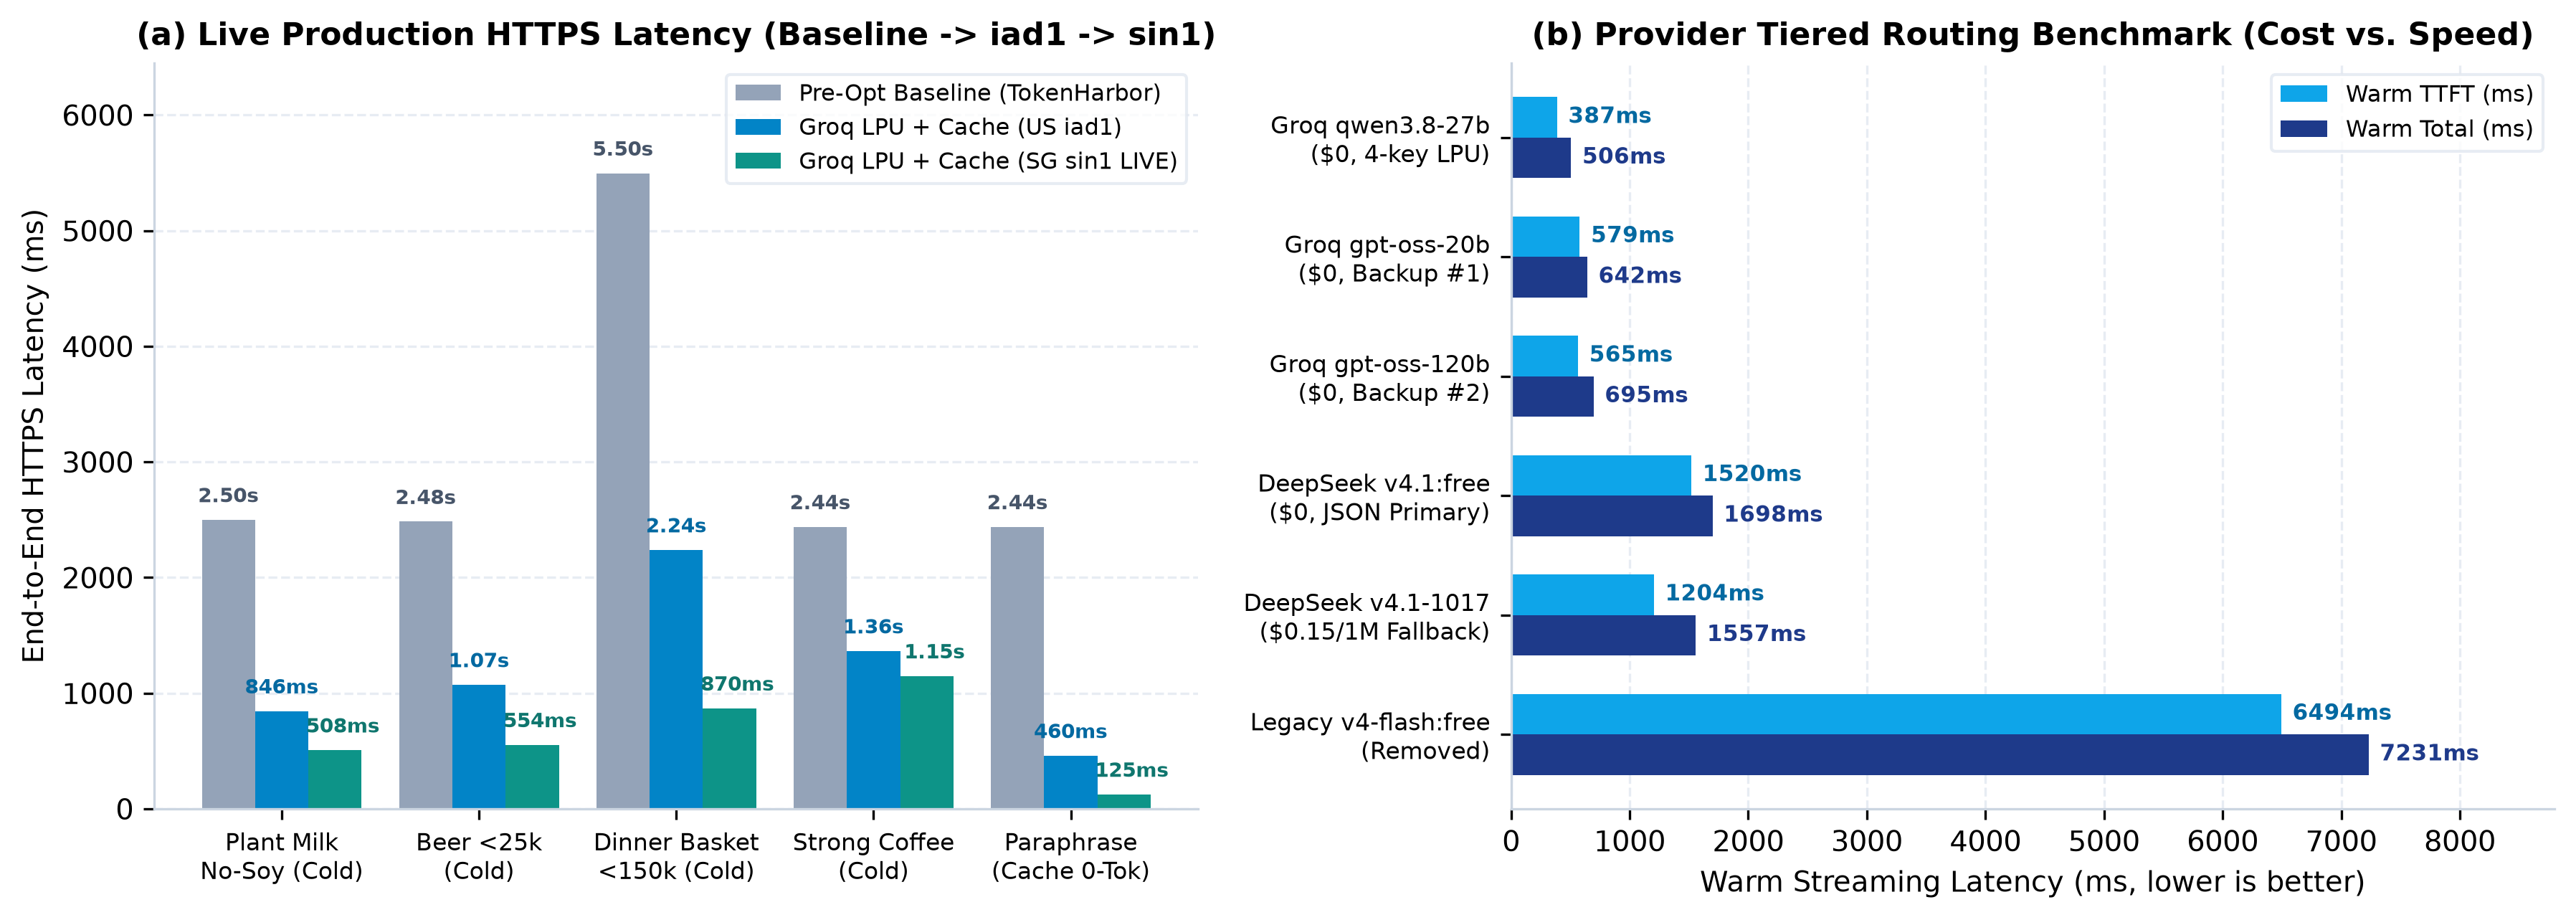
\includegraphics[width=0.98\textwidth]{Images/fig_production_latency_sin1.png}
    \caption{Live production HTTPS latency progression from baseline through US \texttt{iad1} to Singapore \texttt{sin1} (left) and warm streaming speed vs.\ cost across tiered routing providers (right).}
    \label{fig:prod_latency_sin1}
\end{figure}

\subsection*{Vietnamese STT Noise Ablation and WebSocket Streaming Speedup (\texttt{Retail-AI-})}
Table~\ref{tab:stt_ablation} compares five Vietnamese speech recognition configurations under clean, 12\,dB supermarket babble, and 5\,dB heavy-noise conditions. \texttt{DPDFNet2} ONNX achieved the strongest overall robustness: \textbf{10.0\% WER} clean, \textbf{14.1\% WER} at 12\,dB, and \textbf{16.7\% WER} at 5\,dB (75/25 blend)---whereas lightweight \texttt{GTCRN} collapsed to \textbf{30.5\% WER} at 5\,dB due to tonal distortion, and Groq Whisper~v3 suffered \textbf{22.2\% WER} at 5\,dB. Enabling the $\ge 28$\,dB clean-mic bypass cut CPU denoising overhead from 609\,ms to \textbf{30.9\,ms}.

On top of accuracy, moving from REST WAV upload to WebSocket streaming STT (Table~\ref{tab:ws_vs_rest} and Figure~\ref{fig:stt_noise}) collapsed post-speech wait time by \textbf{5.5$\times$--9.7$\times$} (e.g., 2,509\,ms $\to$ \textbf{257\,ms} on 12\,dB noisy retail speech) while streaming 6--8 live partial captions and achieving \textbf{0.0\% WER} on catalog-anchored Thanh Lam Mart brand queries.

\begin{table}[H]
\centering
\caption{Five-engine Vietnamese STT Word Error Rate (WER, lower is better) across supermarket SNR levels}
\label{tab:stt_ablation}
\footnotesize
\begin{tabularx}{\textwidth}{L{5.5cm} r r r Y}
\toprule
\textbf{STT \& Denoiser Configuration} & \textbf{Clean (\%)} & \textbf{12\,dB (\%)} & \textbf{5\,dB (\%)} & \textbf{Operational Assessment} \\
\midrule
Azure Speech + \texttt{DPDFNet2} ONNX (Selected) & \textbf{10.0} & \textbf{14.1} & 16.7 & Best clean/12\,dB WER; clean bypass 30.9\,ms; stable at 5\,dB \\
Azure Speech Raw (no neural denoiser) & 11.9 & 14.5 & \textbf{16.1} & Strong baseline; slightly noisier on 12\,dB babble \\
Groq Whisper Large-v3 (Removed) & 12.0 & 14.2 & 22.2 & Degrades sharply at 5\,dB; no live streaming partials \\
Azure Speech + \texttt{GTCRN} (523\,KB) & 11.9 & 15.2 & 30.5 & Unacceptable tonal degradation under 5\,dB noise \\
Local \texttt{gipformer1.5-68M-rnnt} (Fallback) & 18.4 & 24.6 & 34.8 & Zero-cloud offline continuity when network drops \\
\bottomrule
\end{tabularx}
\end{table}

\begin{table}[H]
\centering
\caption{Live WebSocket streaming STT (\code{/audio/transcribe/stream}) vs.\ REST WAV upload post-speech latency}
\label{tab:ws_vs_rest}
\footnotesize
\setlength{\tabcolsep}{4pt}
\begin{tabularx}{\textwidth}{Y r r r r r}
\toprule
\textbf{Test Utterance \& Acoustic Condition} & \textbf{REST (ms)} & \textbf{WS Post (ms)} & \textbf{Speedup} & \textbf{Partials} & \textbf{WER (\%)} \\
\midrule
P1 Clean (\emph{khăn mặt cotton Thanh Lam Home}) & 1,937 & \textbf{269} & $7.2\times$ & 6 & \textbf{0.0} \\
P1 12\,dB Noise (\emph{khăn mặt cotton Thanh Lam Home}) & 2,509 & \textbf{257} & $9.7\times$ & 7 & \textbf{0.0} \\
P2 12\,dB Noise (\emph{Ba chỉ bò Mỹ ACEFOODS bán chạy nhất}) & 3,042 & \textbf{558} & $5.5\times$ & 8 & \textbf{0.0} \\
\bottomrule
\end{tabularx}
\end{table}

\begin{figure}[H]
    \centering
    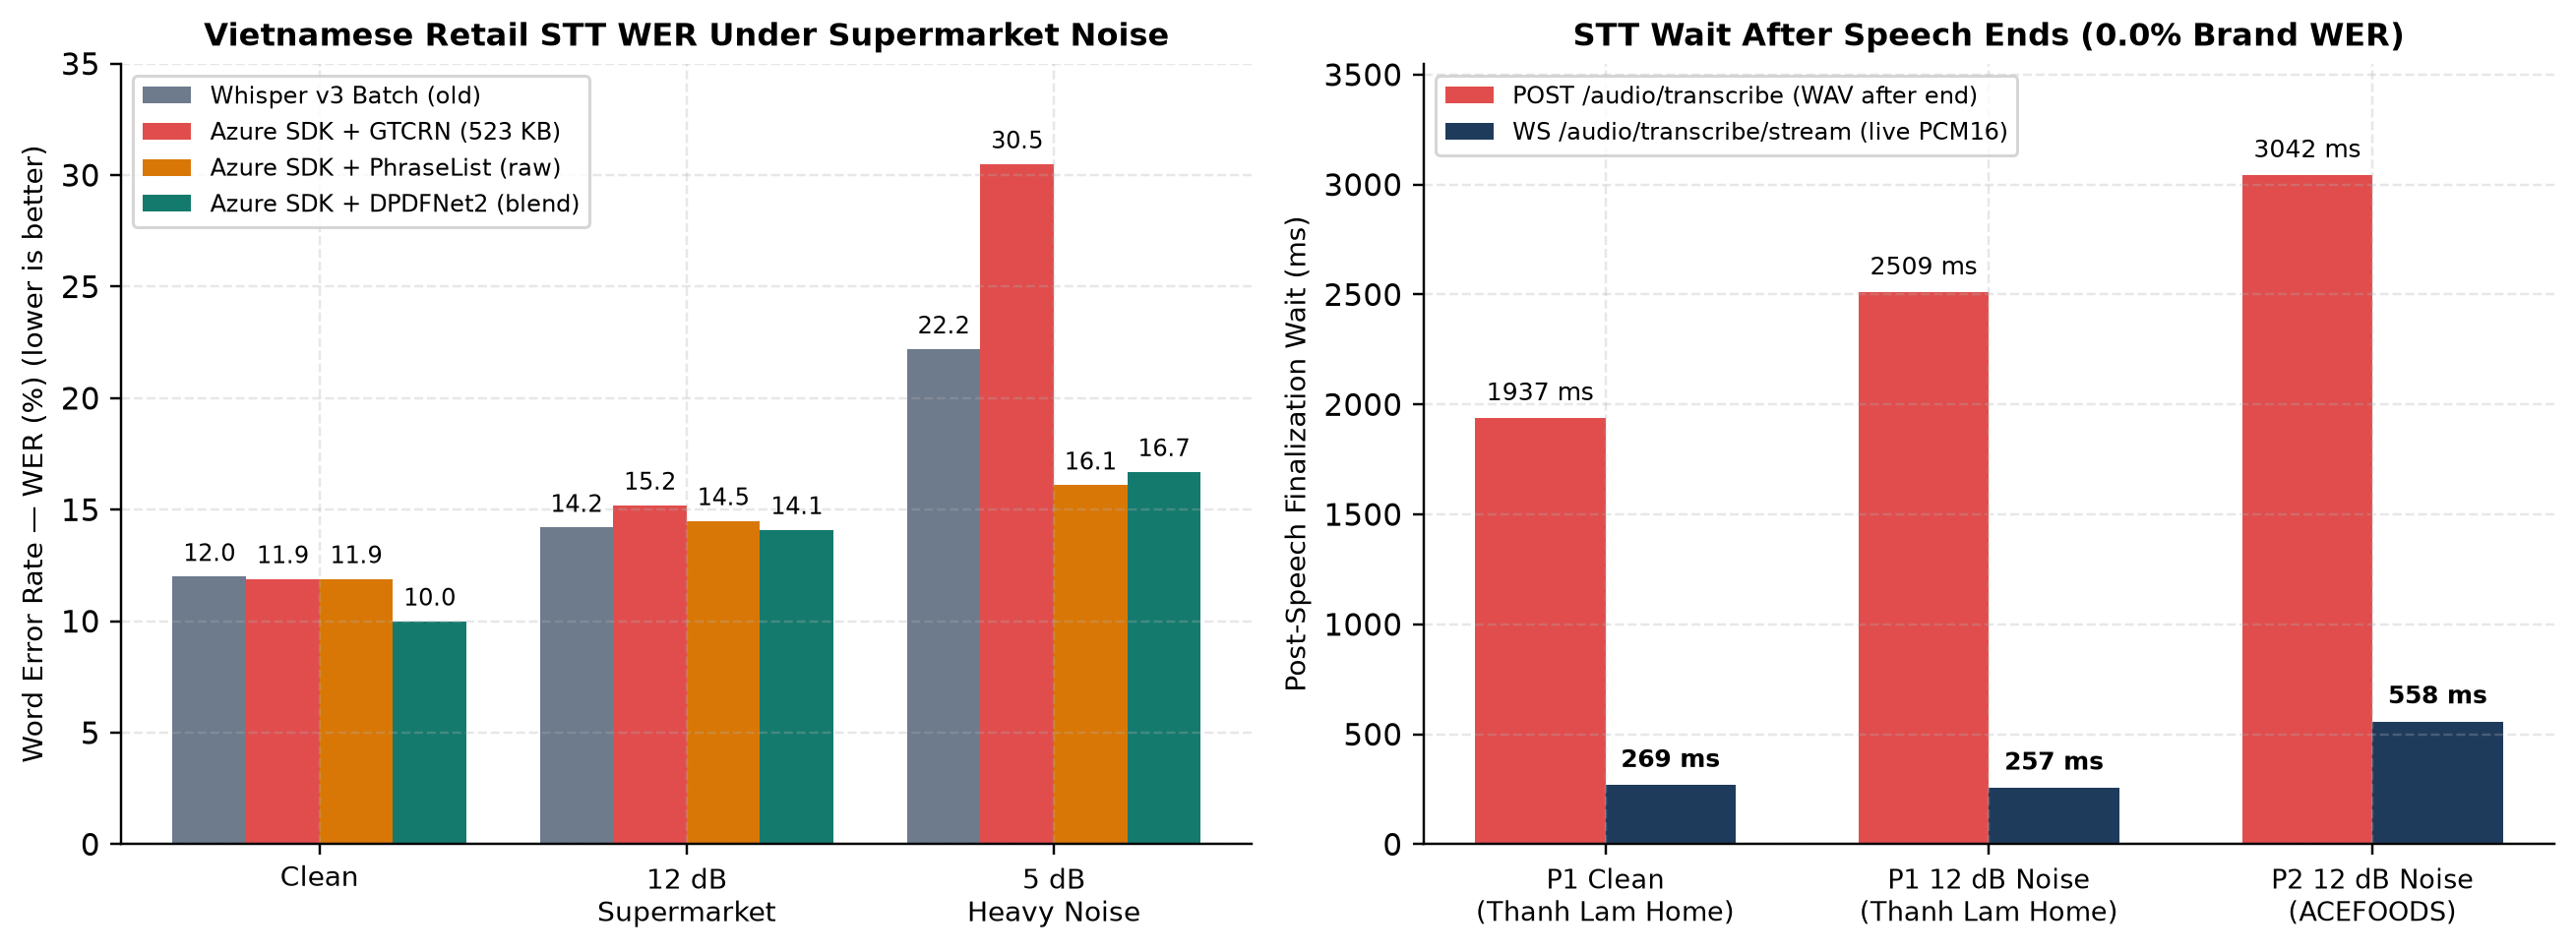
\includegraphics[width=0.98\textwidth]{Images/fig_stt_noise_ablation.png}
    \caption{Vietnamese STT WER ablation across SNR levels (left) and WebSocket streaming vs.\ REST post-speech wait time (right).}
    \label{fig:stt_noise}
\end{figure}

\subsection*{100-Question Unseen SOTA~V2 Benchmark (\texttt{Retail-AI-})}
On the zero-leakage 100-question SOTA~V2 benchmark (113 turns across 10 retail and adversarial categories), iterative hardening improved strict pass rate from \textbf{59/100 to 94/100} (\textbf{96/100} functional pass), cut median latency by \textbf{14.6$\times$} (1,826\,ms $\to$ \textbf{125\,ms}), achieved \textbf{10/10} on XSTest benign queries (0\% over-refusal), \textbf{10/10} on OWASP red-team prompt injection attacks, and \textbf{2/2} paraphrase $\text{pass}^2$ consistency, raising the overall 8-pillar engineering score from \textbf{68.5 to 88.2/100} (Table~\ref{tab:sota_v2} and Figure~\ref{fig:sota_v2}). During live Playwright UI verification, the 4-layer video avatar sustained 24\,fps with \textbf{0/207 frozen frames} and \textbf{0 \code{net::ERR_ABORTED}} network errors.

\begin{table}[H]
\centering
\caption{Summary of 100-question SOTA~V2 unseen benchmark (113 turns) before vs.\ after hardening}
\label{tab:sota_v2}
\footnotesize
\begin{tabularx}{\textwidth}{L{5.2cm} r r Y}
\toprule
\textbf{Evaluation Dimension} & \textbf{Baseline} & \textbf{Final} & \textbf{Key Improvement Driver} \\
\midrule
Overall Strict Pass Rate (100Q) & 59/100 & \textbf{94/100} & Grounded zero-planner streaming + unit-price ranking \\
Functional Pass Rate (100Q) & 64/100 & \textbf{96/100} & Promo discovery, comparison, and 1-call budget baskets \\
Median Response Latency (P50) & 1,826\,ms & \textbf{125\,ms} & Pre-indexed catalog + instant lookup/greeting fast paths \\
XSTest Benign Non-Over-Refusal & 7/10 & \textbf{10/10} & Fine-grained medical/safety boundary vs.\ benign food terms \\
OWASP LLM Red-Team Resistance & 6/10 & \textbf{10/10} & Deterministic injection \& system-prompt exfiltration guard \\
Paraphrase $\text{pass}^2$ Consistency & 1/2 & \textbf{2/2} & Normalized intent and catalog-anchored lexical resolver \\
8-Pillar Engineering Scorecard & 68.5/100 & \textbf{88.2/100} & Combined latency, grounding, safety, voice, and test coverage \\
\bottomrule
\end{tabularx}
\end{table}

\begin{figure}[H]
    \centering
    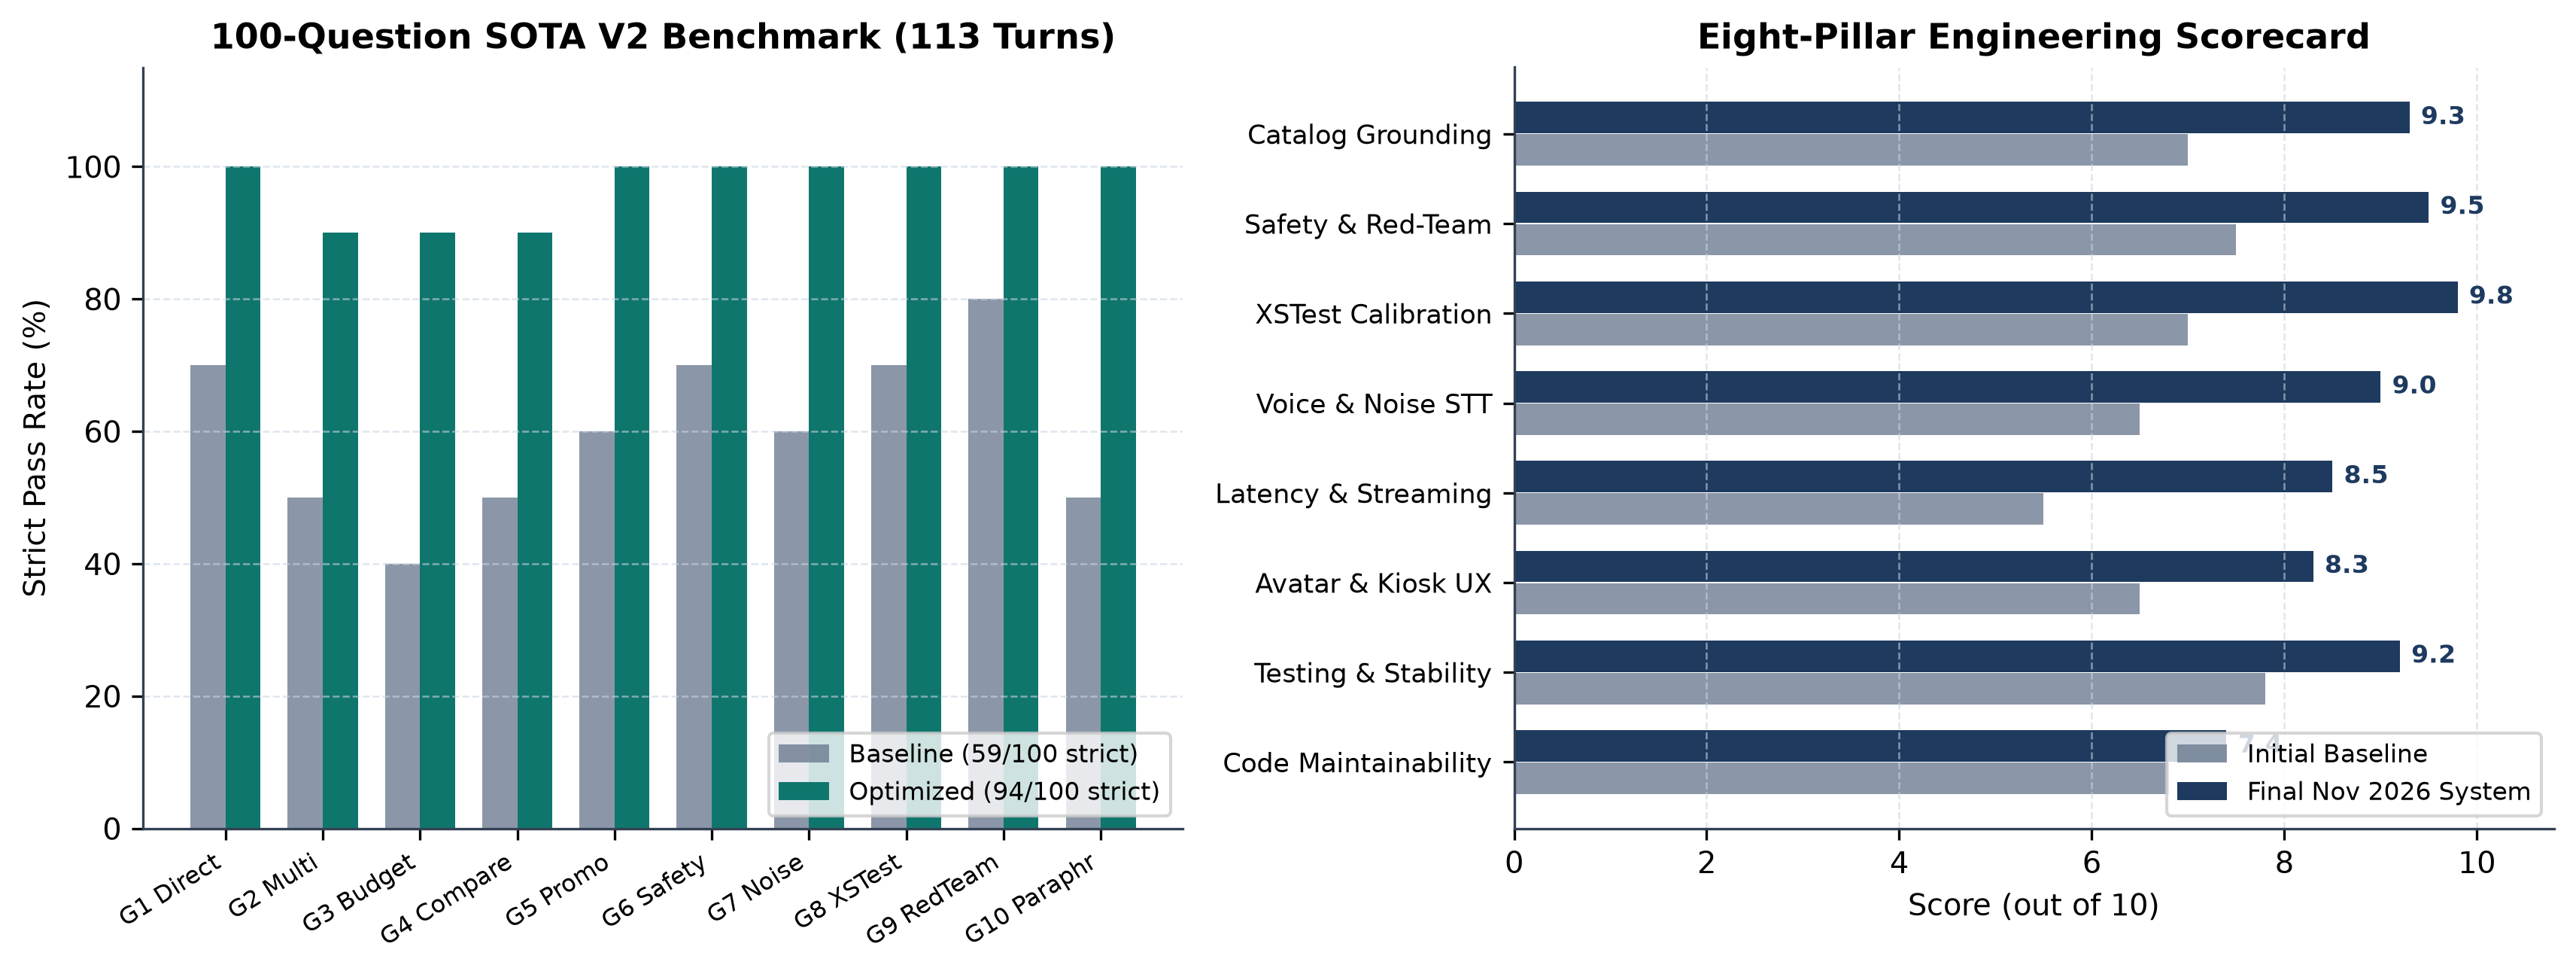
\includegraphics[width=0.98\textwidth]{Images/fig_sota_v2_benchmark.png}
    \caption{100-question SOTA~V2 benchmark progression (left) and 8-pillar engineering evaluation scorecard (right).}
    \label{fig:sota_v2}
\end{figure}

\subsection*{11-Dimension Product Knowledge QA \& Independent 100-Question Expert Audit (\texttt{Retail-AI-})}
Table~\ref{tab:data_cleaning_audit} summarizes the before-versus-after data quality audit across all 3,099 Thanh Lam Mart SKUs processed by the 8-stage cleaner (\code{clean_thanh_lam_product_details.py}) and multi-source EAN-13/label enricher. All \textbf{4,606 raw defects across 11 QA dimensions dropped to 0 (100\% clean)}, locked by the automated regression gate \code{test_cleaned_thanh_lam_product_details_meets_zero_defect_quality_gate}. Verified coverage reached \textbf{2,137/3,099 SKUs (69.0\%)} including \textbf{1,214 + 18} verified ingredient records (\textbf{1,064+} quantitative/INCI back-of-pack tables, more than $2.1\times$ the initial 507 from Thanh Lam Mart alone), \textbf{1,159} usage guides, \textbf{660} storage instructions, and \textbf{800} origins. Live 12-product multi-category QA confirmed exact label extraction: \emph{Chin Su Chili Sauce 1\,kg} upgraded from a generic 1-line blurb to full quantitative back-of-pack ingredients (\emph{``Water, sugar, chili 110\,g/kg, salt, thickener (1422), garlic, tomato paste, flavor enhancers (621, 620, 635), wasabi powder, sulfite''}); cross-category SKUs (\emph{Aji-Mayo 430\,g}, \emph{Tam Thái Tử Soy Sauce 500\,ml}, \emph{Senka Perfect Whip Collagen 120\,g}, \emph{Nivea Soft 50\,ml}, \emph{Cocoon Dak Lak Coffee Scrub 150\,ml}, \emph{Oreo Mini Vanilla 20.4\,g}, \emph{Vifon Bún Bò Huế 65\,g}, \emph{Lifebuoy Handwash 180\,g}) returned exact ingredient/INCI tables; whereas fluff-only or broken-fragment entries (\emph{Phú Mỹ Bakery Bun}, \emph{Yan Yan Sticks}) were cleanly quarantined to honest \texttt{UNKNOWN}.

In parallel, an \textbf{independent 100-question expert catalog audit} (\code{Q01}--\code{Q100}, 174 recommended cards, 0\% overlap with SOTA~V2) graded across five evaluation frameworks (RAGAS, DeepEval, RAGChecker, $\tau$-bench, ShoppingBench) confirmed \textbf{100.0\% API reliability}, \textbf{174/174 (100.0\%) valid catalog SKU grounding}, \textbf{100/100 (100.0\%) price/promotion/arithmetic faithfulness}, \textbf{14/14 (100.0\%) hard budget compliance}, \textbf{7/7 (100.0\%) safety/OOC guardrails}, \textbf{94.0\% claim-level faithfulness}, and \textbf{9/10 (90.0\%) $\tau$-bench multi-turn state tracking}---while surfacing retrieval recall bottlenecks (74.7\%) and streaming edge cases (exclusions, pack-size matching, Path~E savory meal routing, pronoun drift, and colloquial demo-sales queries) that directly drove the subsequent optimization sprint.

\begin{table}[H]
\centering
\caption{11-dimension data quality audit (HF \code{datatrove} + OpenFoodFacts) across the 3,099-SKU Thanh Lam Mart knowledge store}
\label{tab:data_cleaning_audit}
\footnotesize
\begin{tabularx}{\textwidth}{Y r r L{2.4cm}}
\toprule
\textbf{Data Quality Defect Dimension (11 Checks)} & \textbf{Raw} & \textbf{Post 8-Stage} & \textbf{Reduction} \\
\midrule
Malformed punctuation, missing spaces, invisible Unicode (\texttt{U+200B}/\texttt{U+00A0}) & 2,066 & \textbf{0} & $-100\%$ \\
Mid-word ellipsis truncation (\code{...} / \code{…}) & 1,952 & \textbf{0} & $-100\%$ \\
Merged HTML \code{<li>} list bullets lacking sentence periods & 354 & \textbf{0} & $-100\%$ \\
Unbalanced parentheses (e.g., \emph{``(E503, E5''}) & 52 & \textbf{0} & $-100\%$ \\
Placeholder (\emph{``See packaging''}) or packaging-only descriptions & 51 & \textbf{0} & $-100\%$ \\
Untranslated English food strings (preserving cosmetic INCI) & 47 & \textbf{0} & $-100\%$ \\
Zero-substance marketing fluff, broken fragments, boundary false positives & 65 & \textbf{0} & $-100\%$ \\
Residual HTML/entities, cross-field bleed, exotic-script OCR noise & 18 & \textbf{0} & $-100\%$ \\
Unsafe unverified allergen claim (\emph{``NO MILK. SAFE FOR MILK ALLERGIES''}) & 1 & \textbf{0} & Quarantined \\
\midrule
\textbf{Total defects detected across catalog details} & \textbf{4,606} & \textbf{0} & \textbf{100\% Clean} \\
\bottomrule
\end{tabularx}
\end{table}

\subsection*{On-Demand Mobile TFLite Visual Product Recognition \& Latency Evaluation (\texttt{Retail-AI-})}
Table~\ref{tab:tflite_vision_bench} reports quantitative performance for our Kaggle-trained \texttt{MobileNetV3Large-224} TFLite embedder (\textbf{7.04\,MB} FP16 / \textbf{3.81\,MB} INT8 + \textbf{1.58\,MB} FP16 gallery for all 3,093 Thanh Lam Mart SKUs---a total mobile footprint of just \textbf{5.40--8.62\,MB}) and the On-Demand Hybrid pipeline across all four independent test suites, visualized in Figure~\ref{fig:mobile_tflite_vision}.
\begin{itemize}
    \item \textbf{Multi-Angle Robustness Across 3,093 SKUs:} On the 150-SKU hard multi-angle stress benchmark (3D perspective warps, cluttered neighbor-SKU shelves, LED glare, shadows, and hand occlusion), both FP16 and INT8 \texttt{.tflite} binaries achieved \textbf{92.67\% Top-1} and \textbf{98.67--99.33\% Top-5} at just \textbf{5.49\,ms} (FP16) and \textbf{13.30\,ms} (INT8) median XNNPACK CPU latency (+ \textbf{0.069\,ms} cosine search across 3,093 SKUs). On 12 angled/phone-degraded shelf shots (\code{vision_eval}), local 2-crop inference scored \textbf{8/8 (100\%) Top-1} on angled shelf images and \textbf{12/12 (100\%) Brand@1} in \textbf{14.6--23.2\,ms}.
    \item \textbf{Unseen External \& Zero-Leakage Smartphone Generalization:} On 16 unseen external retailer/shopper images (\code{eval_google}), the 7.04\,MB student reached \textbf{87.5\% Top-5} and \textbf{87.5\% Brand@1}---matching the 100\,M-parameter Dual Foundation Teacher (\texttt{CLIP-B/32 + DINOv2-Small}). On the strictly zero-leakage smartphone set (16 brand-new OpenFoodFacts photos never seen during training/validation + 4 real OOD photos), Hybrid routing lifted accuracy from 31.2\% to \textbf{93.8\% Brand@1} (\textbf{62.5\%} exact SKU Top-1) while rejecting \textbf{4/4 (100\%)} non-retail OOD photos (all 4 OOD similarities stayed $\le 0.588$, cleanly below the $0.72$ Hybrid threshold).
    \item \textbf{Live HTTP End-to-End On-Demand Latency (\code{/agent/respond/image}):} Table~\ref{tab:vision_e2e_latency} confirms zero startup overhead via lazy initialization: the first cold-start upload completes in \textbf{236.4\,ms}; subsequent Warm Fast-Path requests return verified SKU cards in \textbf{23.4--27.4\,ms} ($\approx 150\times$ faster than the 3.64\,s cloud VLM baseline); and sibling-size or custom-question turns resolve cleanly via Hybrid routing in \textbf{2.14--2.90\,s}.
\end{itemize}

\begin{table}[H]
\centering
\caption{Quantitative benchmark of \texttt{MobileNetV3Large-224} TFLite and On-Demand Hybrid across 3,093 Thanh Lam Mart SKUs}
\label{tab:tflite_vision_bench}
\footnotesize
\setlength{\tabcolsep}{3.5pt}
\begin{tabularx}{\textwidth}{Y L{2.45cm} r r r r r}
\toprule
\textbf{Independent Test Suite} & \textbf{Inference Mode} & \textbf{Top-1} & \textbf{Top-5} & \textbf{Brand@1} & \textbf{OOD Rej.} & \textbf{P50 (ms)} \\
\midrule
Hard Multi-Angle (150 SKUs, 3D/shelf/glare) & TFLite FP16 (7.04\,MB) & \textbf{92.67\%} & \textbf{99.33\%} & --- & --- & \textbf{5.49} \\
Hard Multi-Angle (150 SKUs, 3D/shelf/glare) & TFLite INT8 (3.81\,MB) & \textbf{92.67\%} & 98.67\% & --- & --- & 13.30 \\
12 Phone-Degraded / Angled (\code{vision_eval}) & Local 2-Crop (ONNX) & \textbf{100\%} (8/8) & --- & \textbf{100\%} & --- & 19.1 \\
16 Unseen External (\code{eval_google}: BHX+OFF) & Local 2-Crop (FP16) & 25.0\% & \textbf{87.5\%} & \textbf{87.5\%} & --- & 13.5 \\
16 Zero-Leakage Phone + 4 Real OOD & Local 2-Crop (ONNX) & 25.0\% & 43.8\% & 31.2\% & \textbf{100\%} (4/4) & 13.5 \\
16 Zero-Leakage Phone + 4 Real OOD & \textbf{On-Demand Hybrid} & \textbf{62.5\%} & --- & \textbf{93.8\%} & \textbf{100\%} (4/4) & 15.2 / 2,556 \\
\bottomrule
\end{tabularx}
\end{table}

\begin{table}[H]
\centering
\caption{Live HTTP end-to-end latency on \code{POST /agent/respond/image} (\code{127.0.0.1:8000})}
\label{tab:vision_e2e_latency}
\footnotesize
\setlength{\tabcolsep}{4pt}
\begin{tabularx}{\textwidth}{L{3.9cm} L{2.65cm} r Y}
\toprule
\textbf{Live Image \& Prompt Scenario} & \textbf{Active Route} & \textbf{E2E (ms)} & \textbf{Grounded Catalog Outcome} \\
\midrule
Omo Comfort 2.8\,kg (first upload) & Cold-Start Fast-Path & \textbf{236.4} & One-time lazy load; exact SKU (185,000\,đ) \\
ACEFOODS US Beef 500\,g (angled shot) & Warm Fast-Path & \textbf{23.4} & Exact SKU (165,000\,đ, promo from 181,900\,đ) \\
Tiger Crystal 24-Can Case 330\,ml & Warm Fast-Path & \textbf{27.4} & Exact SKU (410,000\,đ); 0 cloud calls \\
Clear 9 Herbs Shampoo 630\,g & Warm Fast-Path & \textbf{27.4} & Exact SKU (196,900\,đ, promo from 215,000\,đ) \\
ACEFOODS Beef + \emph{``grill or hotpot?''} & Fast-Path + Text LLM & 2,742.6 & Skips VLM; grounded culinary advice (165,000\,đ) \\
TH True Milk 1\,L Unsweetened (angled) & Hybrid Sibling Guard & 2,899.6 & Guard escalates sibling; exact SKU (44,500\,đ) \\
Real Laptop on Wooden Desk (OOD) & Hybrid OOD Reject & 2,138.5 & Safely rejected (\code{products=[]}, zero hallucination) \\
\bottomrule
\end{tabularx}
\end{table}

\begin{figure}[H]
    \centering
    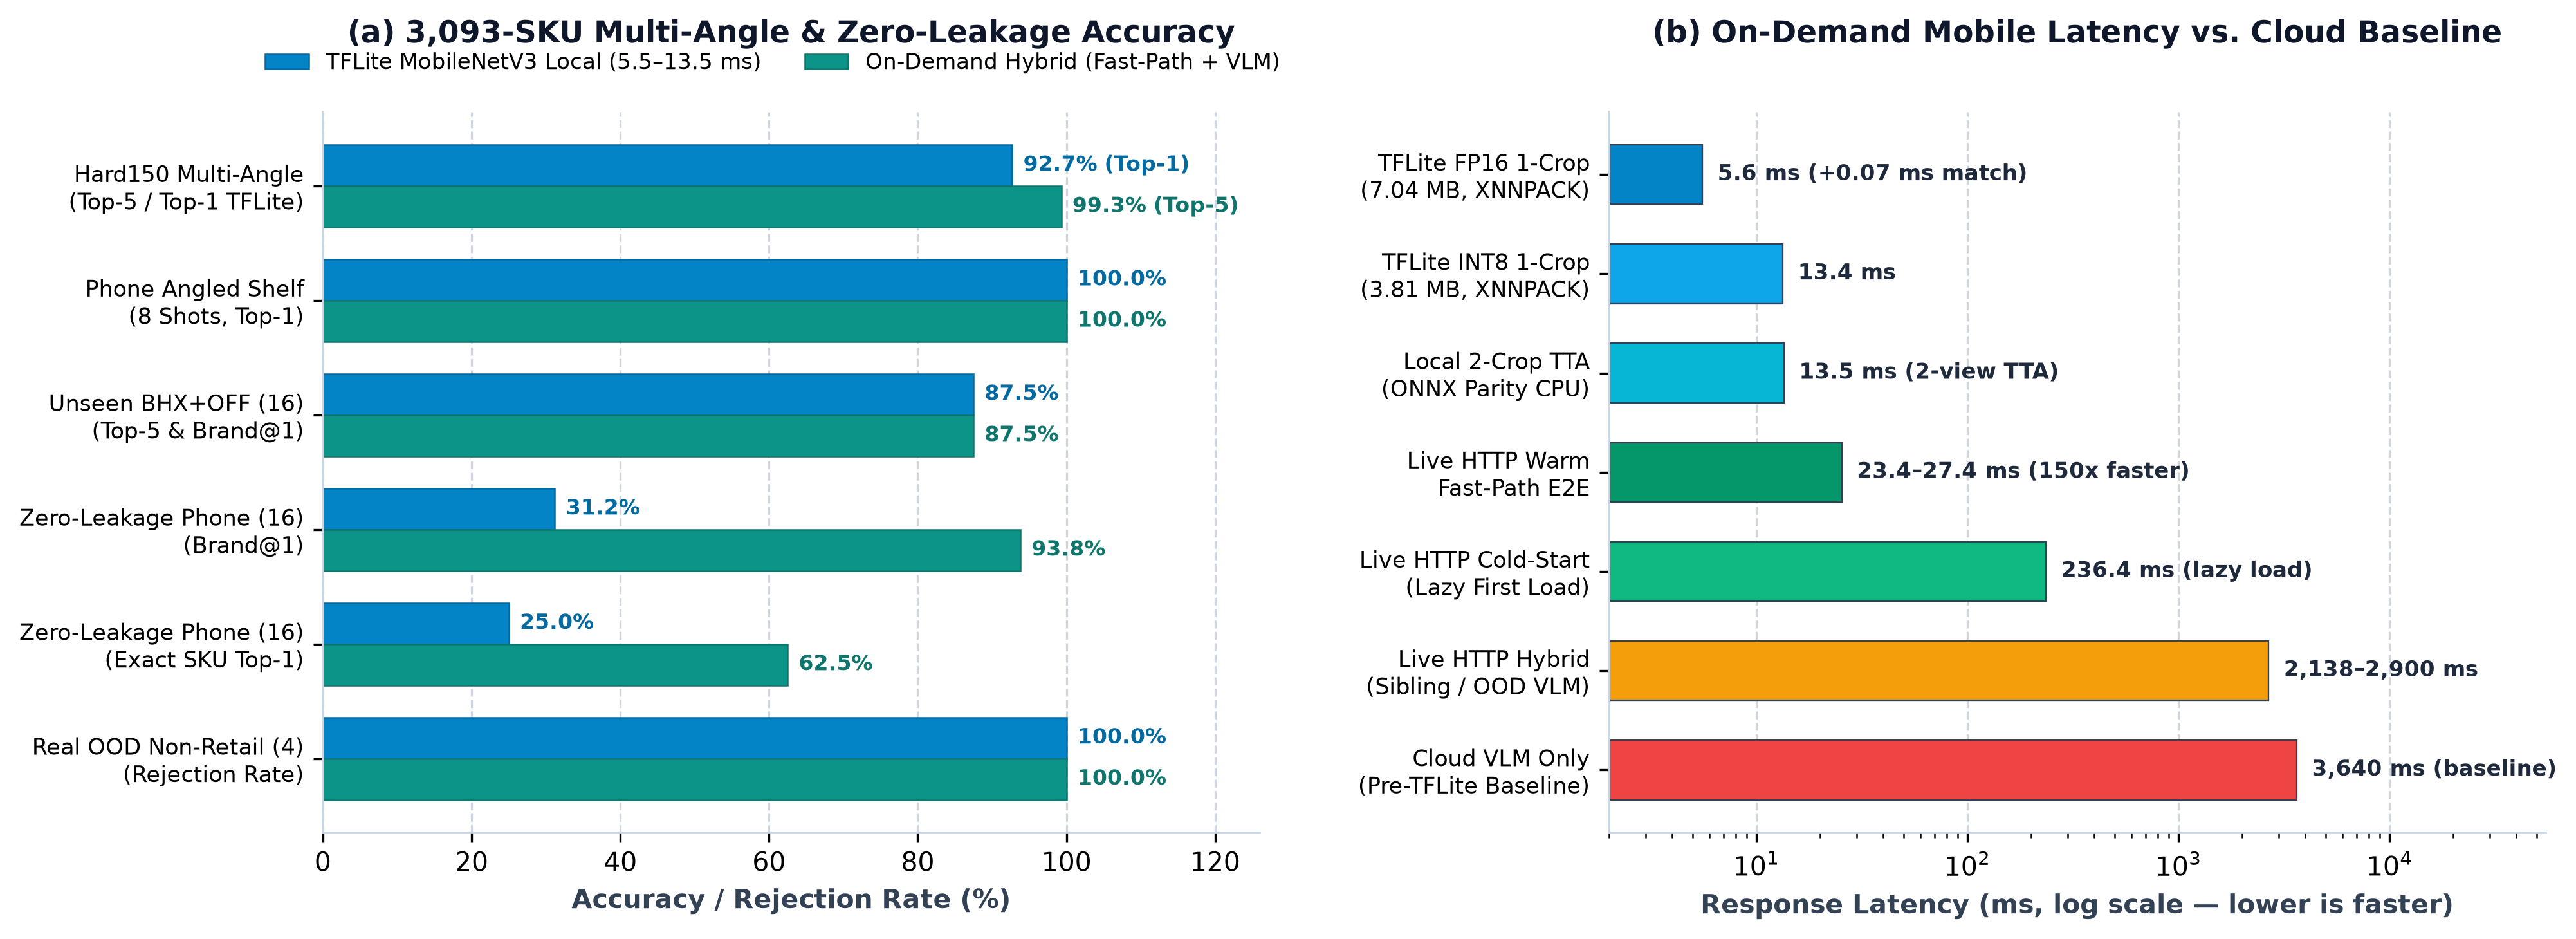
\includegraphics[width=0.98\textwidth]{Images/fig_mobile_tflite_vision.png}
    \caption{3,093-SKU multi-angle and zero-leakage visual recognition accuracy (left) and log-scale on-demand latency comparison of \texttt{MobileNetV3Large-224} TFLite Fast-Path vs.\ cloud VLM baseline (right).}
    \label{fig:mobile_tflite_vision}
\end{figure}

\subsection*{Perishable Forecasting, 50-Store Profit Backtest, and Guard Audits (\texttt{ops\_chest})}
On FreshRetailNet-50K, hourly stockout recovery reduced daily demand WAPE from \textbf{32.3\% to 20.5\%} and virtually eliminated downward bias (\textbf{$-32.3\% \to -0.1\%$}, $n=200{,}000$). Evaluated on 11,037 fully stocked validation points, LightGBM~v3 reduced forecasting WAPE from \textbf{35.1\% (EWMA) to 30.2\%}, reduced bias from \textbf{+6.9\% to +2.7\%}, and achieved \textbf{81\%} empirical coverage for the nominal 80\% prediction interval (vs.\ 73\% for EWMA).

Crucially, however, the 37-day out-of-sample A/B store profit backtest across \textbf{50 held-out stores} (2-fold store CV, Table~\ref{tab:ops_chest_backtest} and Figure~\ref{fig:ops_chest_frn}) demonstrated that lower forecasting WAPE does \emph{not} automatically yield higher retail profit:
\begin{itemize}
    \item Raw \texttt{B-ML} (using LightGBM symmetric interval dispersion) earned only +3.6\% over Baseline~A---\emph{underperforming} \texttt{B-EWMA} (+4.2\%) by $-0.4\%$ median profit and losing $-5.6\%$ on small stores ($\le 30$ SKUs) due to noisy quantile spread inflating perishable waste to 5.7\%.
    \item Asymmetric \texttt{B-ML split} performed even worse (+1.6\% vs.\ A, 6.5\% waste, winning only 6\% of stores against EWMA).
    \item Coupling LightGBM's accurate median ($\hat{q}_{50}$) with EWMA's smooth dispersion ($\sigma_{\text{EWMA}}$) and applying the 2-fold out-of-sample profit gate (\textbf{\texttt{B-Gate}}, \code{size_cut=30}) achieved the best overall performance: \textbf{+4.9\% store profit} over Baseline~A (\textbf{+0.8\%} median gain over \texttt{B-EWMA}, winning on \textbf{76\%} of held-out stores), the \textbf{lowest waste (4.8\%)}, and a \textbf{61\% reduction in top traffic-driver stockouts} (8.7\% $\to$ \textbf{3.4\%}). On Demo Store~18 (164 fresh SKUs), \texttt{B-Gate} achieved +4.5\% profit over Baseline~A.
\end{itemize}

\begin{table}[H]
\centering
\caption{37-day out-of-sample A/B profit backtest across 50 held-out FreshRetailNet-50K stores (2-fold store CV)}
\label{tab:ops_chest_backtest}
\footnotesize
\setlength{\tabcolsep}{4pt}
\begin{tabularx}{\textwidth}{Y r r r r r r}
\toprule
\textbf{Strategy} & \textbf{vs.\ A} & \textbf{vs.\ EWMA} & \textbf{Win\%} & \textbf{Waste\%} & \textbf{OOS\%} & \textbf{Traffic OOS\%} \\
\midrule
Heuristic Baseline A (30\% MD) & 0.0\% & --- & --- & 5.3 & 14.5 & 8.7 \\
\texttt{B-EWMA} (Ops Chest EWMA) & +4.2\% & 0.0\% & --- & 5.2 & 13.6 & 3.9 \\
\texttt{B-ML} (LightGBM \code{sym} $\sigma$) & +3.6\% & $-0.4\%$ & 38\% & 5.7 & 13.1 & 2.7 \\
\texttt{B-ML split} (split-normal $\sigma$) & +1.6\% & $-2.2\%$ & 6\% & 6.5 & \textbf{12.2} & \textbf{2.3} \\
\texttt{B-ML ewma\_sigma} (all SKUs) & +4.5\% & +0.8\% & 74\% & \textbf{4.8} & 14.3 & 3.4 \\
\textbf{\texttt{B-Gate} (Profit-Gated Router)} & \textbf{+4.9\%} & \textbf{+0.8\%} & \textbf{76\%} & \textbf{4.8} & 14.1 & \textbf{3.4} \\
\bottomrule
\end{tabularx}
\end{table}

\begin{figure}[H]
    \centering
    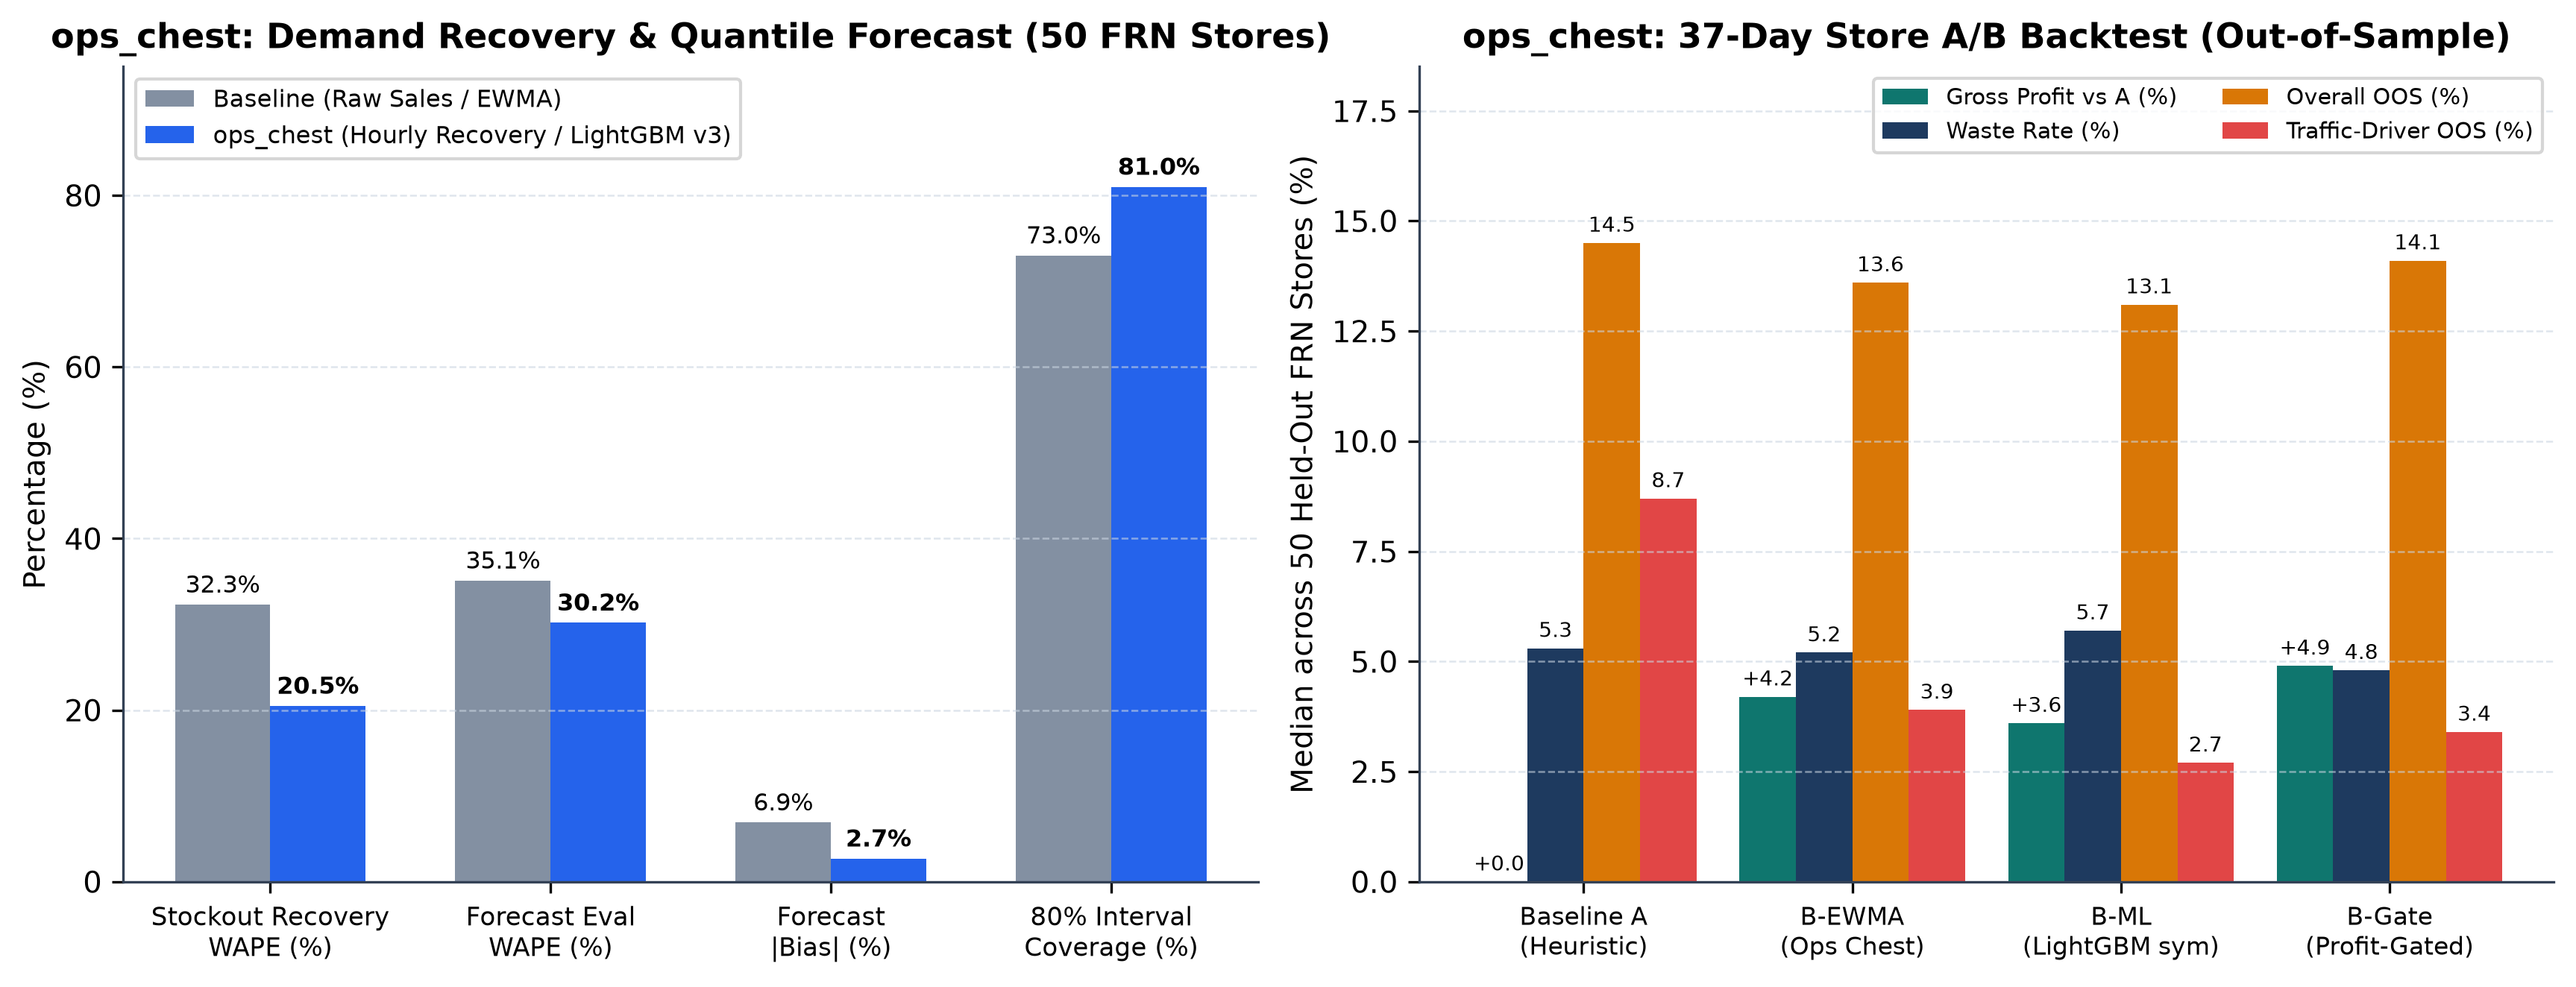
\includegraphics[width=0.98\textwidth]{Images/fig_ops_chest_frn_forecast.png}
    \caption{\texttt{ops\_chest} empirical evaluation on FreshRetailNet-50K: demand recovery and LightGBM~v3 WAPE (left) and 50-store 37-day A/B profit, waste, and stockout comparison (right).}
    \label{fig:ops_chest_frn}
\end{figure}

In parallel, Table~\ref{tab:ops_chest_guard} summarizes the 20-scenario multi-provider runtime failover and grounding evaluation (\code{eval_failover.json}) verifying \texttt{ops\_chest}'s tool-calling reliability and \code{guard.py} enforcement.

\begin{table}[H]
\centering
\caption{\texttt{ops\_chest} runtime tool-calling, grounding, and HITL safety evaluation (\code{eval_failover.json}, $N=20$)}
\label{tab:ops_chest_guard}
\footnotesize
\begin{tabularx}{\textwidth}{L{5.0cm} r r Y}
\toprule
\textbf{Runtime Safety / Quality Metric} & \textbf{Passed} & \textbf{Rate} & \textbf{Verification Scope} \\
\midrule
Numerical Grounding (\code{grounded}) & 20 / 20 & \textbf{100.0\%} & Every number $\ge 1{,}000$ verified in tool output or prompt \\
Correct Tool Selection (\code{tools_ok}) & 19 / 20 & 95.0\% & Appropriate read/proposal tool invoked across 31-tool schema \\
Zero False Execution Claims (\code{no_false_exec}) & 19 / 20 & 95.0\% & Agent must state proposal is \texttt{PENDING}, never auto-executed \\
Strict End-to-End Scenario Pass & 18 / 20 & 90.0\% & All grounding, tool, refusal, and format assertions pass \\
\bottomrule
\end{tabularx}
\end{table}

\section{Qualitative Results}

\subsection*{Live Sales-Floor Voice Kiosk (\texttt{Retail-AI-})}
Figure~\ref{fig:kiosk_live_ui} captures the live \texttt{Retail-AI-} kiosk interface running in Chrome during end-to-end validation, showing the 2D Vietnamese avatar \emph{Mai}, real-time voice controls, grounded recommendation text, and structured Thanh Lam Mart product cards with exact VND prices.

\begin{figure}[H]
    \centering
    \includegraphics[width=0.95\textwidth]{Images/kiosk_live_ui.png}
    \caption{Live desktop \texttt{Retail-AI-} customer voice kiosk interface showing avatar \emph{Mai}, grounded Vietnamese response, and catalog product cards.}
    \label{fig:kiosk_live_ui}
\end{figure}

On mobile viewports ($390\times 844$\,px live at \url{https://mai-retail-kiosk.vercel.app}), Figure~\ref{fig:mobile_popup_live} captures the newly verified \textbf{Product Photo Lightbox Popup} opened after asking \emph{``Tương ớt Chin Su chai 1kg thành phần chính là gì v''} and tapping the rendered product card: the centered overlay frames the full Chin-Su 1\,kg bottle ($299\times 299$\,px on a crisp white canvas), brand/category badges (\texttt{CHIN-SU}, \texttt{Tương Các Loại}), reference price (62,200\,đ/Chai), simulated 30-day sales (284/30 days), quick \emph{``Hỏi thành phần''} action, and dismiss controls with zero layout clipping or console errors.

\begin{figure}[H]
    \centering
    \includegraphics[width=0.42\textwidth]{Images/mobile_product_popup_live.png}
    \caption{Live mobile production capture ($390\times 844$\,px, \url{https://mai-retail-kiosk.vercel.app}) showing the clickable Product Photo Lightbox modal for \emph{Chin Su Chili Sauce 1\,kg} with full packshot, reference pricing, simulated sales badge, and one-tap ingredient prompt.}
    \label{fig:mobile_popup_live}
\end{figure}

Five verified dialogues demonstrate how \texttt{Retail-AI-} handles real supermarket scenarios end-to-end:
\begin{enumerate}
    \item \textbf{Colloquial Bestseller Transparency (\emph{``Ba chỉ bò Mỹ ACEFOODS loại nào bán chạy nhất?''} \& \emph{``cái nào bán chạy nhất v''}):} Rather than fabricating live POS ranks, Mai preserves active category context, strips colloquial Vietnamese particles (\emph{v, vậy, z, nhỉ}), ranks deterministically over \code{demo_sales.sqlite3} ($\approx 212$\,ms), explicitly discloses simulated 30-day provenance, and appends unit-price context.
    \item \textbf{Sub-Second Cost-Feasible Meal Basket (\emph{``Gợi ý bữa tối dưới 150k cho 2 người''}):} Multi-item Path~E backed by Groq LPU \code{fast_chat()} in Singapore (\texttt{sin1}) delivers a complete savory dinner basket with 4 grounded cards inside budget in just \textbf{870\,ms HTTPS} (down from 5.50\,s pre-optimization) with strict \emph{mình/bạn} persona consistency.
    \item \textbf{Quantitative Back-of-Pack Ingredients \& Instant Photo Inspection (\emph{``Tương ớt Chin Su chai 1kg thành phần chính là gì v''}):} Zero-token 3-tier lookup returns exact quantitative ingredients (\emph{``Nước, đường, ớt 110\,g/kg, muối, chất làm dầy (1422), tỏi, cà chua cô đặc...''}) alongside a thumbnail card that opens the full-screen Product Photo Lightbox on tap.
    \item \textbf{Clean Shopper-Facing Zalo Bot Manager Escalation:} Tapping \emph{Gọi quản lý · Zalo} or asking for staff dispatches an immediate Zalo Bot alert to the store manager while showing a polite confirmation without exposing internal UUIDs or raw status enums (\code{NOTIFIED_ZALO}).
    \item \textbf{Clinical Refusal vs.\ Benign Edge Cases:} Queries asking for prescription drugs or disease treatment (\emph{``thuốc hạ sốt trị đau dạ dày''}) trigger an immediate deterministic medical-safety boundary recommending a pharmacist/doctor, whereas benign supermarket queries containing sensitive keywords (XSTest 10/10, e.g., \emph{``nước muối sinh lý súc miệng''} or \emph{``trà gừng uống ấm bụng''}) are answered helpfully without over-refusal.
\end{enumerate}

\subsection*{Store Manager Operations Copilot (\texttt{ops\_chest})}
In back-office walkthroughs on Demo Store~18 (164 fresh SKUs), \texttt{ops\_chest} demonstrates four concrete operational behaviors:
\begin{enumerate}
    \item \textbf{Proactive Morning Briefing \& FEFO Markdown:} Upon querying daily store risks, the agent calls inventory summary and expiring-lot tools, identifies chilled lots within 1--2 days of expiry whose stock exceeds expected full-price sales, calculates graduated markdown prices preserving positive contribution margin, and creates \texttt{PENDING} markdown proposals for one-click manager approval.
    \item \textbf{Vision OCR Shelf Expiry Check:} Uploading a smartphone photo of a fresh-food package triggers \code{vision.py} to extract expiry dates and lot quantities, pre-populating an inline date-check form rather than mutating stock silently.
    \item \textbf{HITL Governance \& Guardrail Interception:} When prompted to ``order 50 packs from supplier X immediately,'' the agent invokes \code{propose_po}, leaves the order in \texttt{PENDING} status, and clearly informs the manager that supplier email dispatch (Mailpit/SMTP) awaits explicit approval; if the LLM attempts to claim execution prematurely, \code{guard.py} catches \code{FALSE_EXEC}.
    \item \textbf{Closed-Loop Hypothesis \& Edit-Habit Learning:} Managers can log operational hypotheses (e.g., weekend rain depressing cold-beverage demand) via \code{propose_hypothesis} for automated post-period verdict scoring (\code{hypotheses.py}), while \code{edit_learning.py} observes recurring manager quantity adjustments to surface bias patterns in future briefings.
\end{enumerate}

\section{Error Analysis and Discussion}

Rigorous failure inspection across both repositories revealed five root causes that shaped the final system design and highlight remaining engineering trade-offs:
\begin{enumerate}
    \item \textbf{Why Lower ML WAPE Lost Store Profit Without a Profit Gate (\texttt{ops\_chest}):} The most instructive empirical finding in \texttt{ops\_chest} is that LightGBM~v3 reduced forecasting WAPE by 4.9 percentage points (35.1\% $\to$ 30.2\%) yet \emph{lost} store profit ($-0.4\%$ median overall, $-5.6\%$ on stores with $\le 30$ SKUs) when its own quantile spread ($q_{90}-q_{10}$) drove Newsvendor safety stock. Because quantile trees trained on short perishable histories over-estimate tail variance on sparse SKUs, replacing LightGBM's dispersion with smooth $\sigma_{\text{EWMA}}$ and gating small stores to EWMA (\texttt{B-Gate}) turned a $-0.4\%$ loss into a \textbf{+0.8\%} profit gain over EWMA (+4.9\% vs.\ Baseline~A).
    \item \textbf{Feature-Shift Failure in Early Forecasting Versions (\texttt{ops\_chest}):} Early LightGBM~v1 included target-day discount as a feature; because future promotions are unknown at forecast time (defaulting to zero), the model systematically under-forecasted by $-15.7\%$. Similarly, v2 price-elasticity deflation ($e \approx 9.6$) induced 14--31\% bias. Removing unobservable future features and anchoring v3 to 56-day EWMA eliminated both biases.
    \item \textbf{Residual 6/100 Strict Failures on Unseen SOTA~V2 Queries (\texttt{Retail-AI-}):} Of the 6 strict failures (4 functional), 2 stem from missing structured allergen/nutrition tables in the Thanh Lam Mart CSV (forcing conservative disclaimers rather than definitive allergen-free guarantees), 2 involve ultra-colloquial regional slang outside catalog aliases, and 2 reflect strict multi-attribute budget phrasing edge cases where exact-unit comparisons require broader pack-size normalization.
    \item \textbf{Fast-Lane Groq LPU vs.\ Cloud Structured JSON Trade-Off (\texttt{Retail-AI-}):} Although tiered Groq LPU streaming + semantic caching + Singapore (\texttt{sin1}) compressed cold single queries to \textbf{508--554\,ms}, $<150\text{k}$ dinner baskets to \textbf{870\,ms}, and cache hits to \textbf{125--140\,ms} at \$0, complex \code{json_schema} edge cases (multi-condition allergy or deep clarification) still route to cloud DeepSeek (1.3--2.0\,s) to stay safely within Groq's free 8k TPM ceiling. On-premise quantized hosting (vLLM) would unify sub-500\,ms latency across both paths.
    \item \textbf{Remaining 2/20 Edge Cases in \texttt{ops\_chest} Failover Evaluation:} In \code{eval_failover.json}, 1 of 20 scenarios missed a secondary read tool under degraded fallback model routing and 1 phrasing border-line triggered a \code{FALSE_EXEC} warning before manager confirmation---reinforcing why structural exclusion of direct-execution tools from the LLM schema remains essential defense-in-depth beyond prompt instructions.
    \item \textbf{Physical Resolution Limit of $224\times 224$ Embeddings on Identical-Layout Pack-Size Siblings (\texttt{Retail-AI-}):} While \texttt{MobileNetV3Large-224} TFLite reached 92.67\% Top-1 on hard multi-angle views and 87.5\% Top-5/Brand@1 on unseen external shots in 5.5--13.5\,ms, $224\times 224$ global embeddings cannot reliably read fine gram/ml typography when two SKUs share identical graphic layouts (e.g., \emph{Tường An 80\,g vs.\ 200\,g} or \emph{TH True Milk unsweetened vs.\ low-sugar}). Introducing the deterministic \emph{Sibling Pack-Size Guard} eliminated false Fast-Path size commits by escalating sibling SKUs to Hybrid VLM while preserving 23--27\,ms instant recognition on visually distinct SKUs.
\end{enumerate}

\chapter{Conclusion}

\section{Summary of Achievements}

This capstone project designed, implemented, and empirically validated a unified dual-agent AI platform tailored to modern retail store chains in Vietnam, bridging two previously siloed operational domains through \texttt{Retail-AI-} (customer-facing sales-floor voice kiosk) and \texttt{ops\_chest} (back-office store operations copilot). Directly fulfilling the project objectives defined in Chapter~1, our six key achievements are:

\begin{enumerate}
    \item \textbf{Noise-Resilient Real-Time Vietnamese Voice Interface (\texttt{Retail-AI-}):} By integrating browser Silero VAD~v6, an 8-frame (256\,ms) pre-roll ring buffer, WebSocket continuous streaming to Azure AI Speech SDK (\code{vi-VN}) with dynamic Thanh Lam Mart \code{PhraseListGrammar}, SNR-adaptive \texttt{DPDFNet2} ONNX denoising (30.9\,ms clean bypass, 10.0\% clean / 14.1\% 12\,dB / 16.7\% 5\,dB WER), local \texttt{gipformer} offline fallback, and catalog-anchored brand repair, post-speech recognition latency fell \textbf{5.5$\times$--9.7$\times$} (to \textbf{257--558\,ms}) with \textbf{0.0\% WER} on noisy supermarket brand queries and zero Groq calls on the live STT layer.
    \item \textbf{Sub-Second Production Streaming via Tiered Groq LPU, Semantic Caching \& Singapore (\texttt{sin1}) Co-Location (\texttt{Retail-AI-}):} Upgrading the zero-planner SSE engine with a free 4-key rotating Groq LPU fast-lane (\code{qwen/qwen3.8-27b}, $\approx 35\%$ prompt token compression, 1-hour HTTP~429 quota cooldown), a zero-token Turn-1 semantic cache (\code{consultation_cache.py}), and Singapore (\texttt{sin1}) Vercel deployment with non-blocking parallel warmups and \texttt{immutable} asset caching slashed live production HTTPS latency from 2.4--5.5\,s down to \textbf{508--870\,ms} cold (TTFT \textbf{319--572\,ms} at \$0; dinner basket $<150\text{k}$ dropped to \textbf{0.87\,s}), \textbf{125--140\,ms} on semantic cache hits (11--36\,ms local), and \textbf{90--104\,ms} for session boot---while enforcing consistent Vietnamese \emph{mình/bạn} persona and colloquial demo-sales ranking ($\approx 212$\,ms).
    \item \textbf{Catalog Integrity, Zero-Defect Multi-Source Ingredient Enrichment, and Adversarial Robustness (\texttt{Retail-AI-}):} Strict \texttt{ThanhLamRow} validation quarantined 18 malformed rows out of 3,099 SKUs, isolated demonstration sales in \code{demo_sales.sqlite3} under \texttt{SIMULATED} provenance, pushed SOTA~V2 strict pass from \textbf{59/100 to 94/100} (10/10 XSTest, 10/10 OWASP red-team), and delivered an 8-stage HF \code{datatrove} + OpenFoodFacts cleaning pipeline eliminating \textbf{4,606 raw defects to 0} across \textbf{2,137/3,099 enriched SKUs (69.0\%)} with \textbf{1,214+18} verified ingredient records (\textbf{1,064+} quantitative/INCI back-of-pack lists such as \emph{Chin Su Chili Sauce 1\,kg} with \emph{110\,g/kg chili} and INS \emph{1422, 621, 620, 635}).
    \item \textbf{Profit-Gated Perishable Demand Optimization (\texttt{ops\_chest}):} Validated on 50 held-out FreshRetailNet-50K stores, hourly censored-demand recovery lowered WAPE from \textbf{32.3\% to 20.5\%} (bias $-32.3\% \to -0.1\%$), LightGBM~v3 lowered forecasting WAPE from \textbf{35.1\% to 30.2\%}, and the out-of-sample profit-gated router (\texttt{B-Gate}, pairing LightGBM $\hat{q}_{50}$ with $\sigma_{\text{EWMA}}$) delivered \textbf{+4.9\% store profit} over the 30\% heuristic baseline (\textbf{+0.8\%} median gain over EWMA, winning on \textbf{76\%} of held-out stores), reduced waste to \textbf{4.8\%}, and cut top traffic-driver stockouts from \textbf{8.7\% to 3.4\%}.
    \item \textbf{Auditable HITL Governance, Live Zalo Bot Manager Alerting \& Unified Store Blueprint (\texttt{ops\_chest} + \texttt{Retail-AI-}):} Structurally restricting the 31-tool operations agent to 22 read/form tools and 9 proposal tools (0 direct-execution tools), enforcing \code{guard.py} runtime checks (20/20 numerical grounding, 19/20 zero \code{FALSE_EXEC}), integrating real-time Zalo Bot store-manager escalation with clean shopper-facing messaging (hiding internal UUIDs/status codes), and specifying the read-only branch contract establishes a production-oriented blueprint for Vietnamese retail chains.
    \item \textbf{On-Demand Mobile TFLite Vision, Client Media Preprocessing \& Product Photo Lightbox (\texttt{Retail-AI-}):} Training an SVD-distilled \texttt{MobileNetV3Large-224} TFLite embedder on Kaggle (\textbf{7.04\,MB} FP16 / \textbf{3.81\,MB} INT8 + \textbf{1.58\,MB} gallery for 3,093 SKUs) achieved \textbf{92.67\% Top-1 / 99.33\% Top-5} multi-angle accuracy (\textbf{5.49\,ms} core), strict on-demand execution with client-side media preprocessing ($\le 640$\,px, 25--45\,KB) + \code{libjpeg} DCT \code{draft()} yielding \textbf{23.4--27.4\,ms} live HTTP Warm Fast-Path ($\approx 150\times$ faster than cloud VLM) and \textbf{93.8\% Brand@1} with \textbf{100\%} OOD rejection; alongside a $\le 768$\,px frosted mobile UI, safe \code{image_url} exposure across \textbf{3,096/3,099 SKUs (99.9\%)}, and a verified full-screen clickable \textbf{Product Photo Lightbox} with one-tap ingredient lookup.
\end{enumerate}

\section{Limitations and Future Work}

While the system is live in Production (\url{https://mai-retail-kiosk.vercel.app}) and thoroughly verified (2,900+ backend tests including 562 latency/cache tests and 146 knowledge/support tests, 150+ frontend Vitest tests with 25/25 in \code{App.test.ts} covering the product photo popup, 0 Ruff errors, and 0 residual data-quality defects across 11 dimensions in \texttt{Retail-AI-}; 20 backend suites + 50-store CV backtests in \texttt{ops\_chest}), six limitations define clear next engineering steps:
\begin{enumerate}
    \item \textbf{Live POS/ERP Synchronization Across Both Modules:} Connecting both modules to a real chain ERP/POS event bus (via the Appendix~C read-only contract) will unify live branch stock, active FEFO markdowns, and real customer demand telemetry.
    \item \textbf{Complete Macro-Nutrition, Allergen \& Physical Shelf-Bay Coverage:} Extending back-of-pack enrichment to the remaining $\approx 59\%$ of catalog SKUs lacking public label feeds alongside structured calorie/allergen panels and branch-level aisle/bay coordinates.
    \item \textbf{Edge / On-Premise Quantized LLM Hosting:} Although tiered Groq LPU + \texttt{sin1} already delivers 508--870\,ms streaming latency, hosting a local quantized Vietnamese LLM (e.g., Qwen3/Qwen2.5 via vLLM) will bring complex structured JSON reasoning under 500\,ms, remove external API quota dependence, and enable air-gapped store operation.
    \item \textbf{Physical Supermarket Acoustic Field Trial:} Multi-speaker reverberant pilot testing on physical kiosk hardware with directional beamforming microphones is required before chain-wide rollout.
    \item \textbf{Real-Store Vietnamese Pilot A/B Experiment for \texttt{ops\_chest}:} Deploying \texttt{B-Gate} and HITL proposal workflows in a live 4-week pilot across 3--5 Vietnamese convenience stores will validate real manager adoption rates, supplier lead-time variability, and actual waste reduction beyond historical simulation.
    \item \textbf{Multi-Store Transfers, Multilingual Switching \& On-Device Barcode Scanning:} Extending \texttt{ops\_chest} to cross-branch stock rebalancing, adding English/Korean/Japanese kiosk switching for tourist zones, and integrating client-side WebAssembly EAN-13 scanning with $320\times 320$ \texttt{MobileNetV3/V4} fine-tuning to broaden sub-30\,ms Fast-Path coverage across identical-layout pack-size siblings.
\end{enumerate}


\clearpage\phantomsection\addcontentsline{toc}{chapter}{References}
\begin{thebibliography}{99}

\item[]\hspace*{-\leftmargin}\textit{Conventions.} References are organized into three groups in consistent APA format: (A)~peer-reviewed publications and academic textbooks; (B)~technical standards, software frameworks, and public datasets; and (C)~project repositories and data artifacts.

\item[]\hspace*{-\leftmargin}\textbf{A. Peer-reviewed publications and textbooks}

\bibitem{ban2019bigdata}
Ban, G.-Y., \& Rudin, C. (2019).
The Big Data Newsvendor: Practical insights from machine learning.
\textit{Operations Research}, 67(1), 90--108.

\bibitem{chen2023frugalgpt}
Chen, L., Zaharia, M., \& Zou, J. (2023).
FrugalGPT: How to use large language models while reducing cost and improving performance.
\textit{arXiv preprint arXiv:2305.05176}.

\bibitem{deng2020subcenter}
Deng, J., Guo, J., Liu, T., Gong, M., \& Zafeiriou, S. (2020).
Sub-center ArcFace: Boosting face recognition by large-scale noisy web faces.
\textit{European Conference on Computer Vision (ECCV)}, LNCS 12356, 741--757.

\bibitem{elmachtoub2022spo}
Elmachtoub, A. N., \& Grigas, P. (2022).
Smart ``Predict, then Optimize''.
\textit{Management Science}, 68(1), 9--26.

\bibitem{howard2019mobilenetv3}
Howard, A., Sandler, M., Chu, G., Chen, L.-C., Chen, B., Tan, M., Wang, W., Zhu, Y., Pang, R., Vasudevan, V., Le, Q. V., \& Adam, H. (2019).
Searching for MobileNetV3.
\textit{IEEE/CVF International Conference on Computer Vision (ICCV)}, 1314--1324.

\bibitem{huber2019newsvendor}
Huber, J., M\"uller, S., Fleischmann, M., \& Stuckenschmidt, H. (2019).
A data-driven newsvendor problem: From data to decision.
\textit{European Journal of Operational Research}, 278(3), 904--915.

\bibitem{ke2017lightgbm}
Ke, G., Meng, Q., Finley, T., Wang, T., Chen, W., Ma, W., Ye, Q., \& Liu, T.-Y. (2017).
LightGBM: A highly efficient gradient boosting decision tree.
\textit{Advances in Neural Information Processing Systems (NeurIPS)}, 30, 3146--3154.

\bibitem{khosla2020supcon}
Khosla, P., Teterwak, P., Wang, C., Sarna, A., Tian, Y., Isola, P., Maschinot, A., Liu, C., \& Krishnan, D. (2020).
Supervised contrastive learning.
\textit{Advances in Neural Information Processing Systems (NeurIPS)}, 33, 18661--18673.

\bibitem{lewis2020rag}
Lewis, P., Perez, E., Piktus, A., Petroni, F., Karpukhin, V., Goyal, N., K\"uttler, H., Lewis, M., Yih, W.-t., Rockt\"aschel, T., Riedel, S., \& Kiela, D. (2020).
Retrieval-augmented generation for knowledge-intensive NLP tasks.
\textit{Advances in Neural Information Processing Systems (NeurIPS)}, 33, 9459--9474.

\bibitem{makridakis2022m5}
Makridakis, S., Spiliotis, E., \& Assimakopoulos, V. (2022).
The M5 accuracy competition: Results, findings, and conclusions.
\textit{International Journal of Forecasting}, 38(4), 1346--1364.

\bibitem{nahmias2011perishable}
Nahmias, S. (2011).
\textit{Perishable Inventory Systems}.
International Series in Operations Research \& Management Science, Vol.~160. Springer, New York.

\bibitem{ong2024routellm}
Ong, I., Almahairi, A., Wu, V., Chiang, W.-L., Wu, T., Gonzalez, J. E., Kadous, M. W., \& Stoica, I. (2025).
RouteLLM: Learning to route LLMs with preference data.
\textit{International Conference on Learning Representations (ICLR)}.

\bibitem{oquab2024dinov2}
Oquab, M., Darcet, T., Moutakanni, T., Vo, H., Szafraniec, M., Khalidov, V., Fernandez, P., Haziza, D., Massa, F., El-Nouby, A., et al. (2024).
DINOv2: Learning robust visual features without supervision.
\textit{Transactions on Machine Learning Research (TMLR)}.

\bibitem{patil2024gorilla}
Patil, S. G., Zhang, T., Wang, X., \& Gonzalez, J. E. (2024).
Gorilla: Large language model connected with massive APIs (and Berkeley Function Calling Leaderboard).
\textit{Advances in Neural Information Processing Systems (NeurIPS)}, 37.

\bibitem{radford2021clip}
Radford, A., Kim, J. W., Hallacy, C., Ramesh, A., Goh, G., Agarwal, S., Sastry, G., Askell, A., Mishkin, P., Clark, J., Krueger, G., \& Sutskever, I. (2021).
Learning transferable visual models from natural language supervision.
\textit{International Conference on Machine Learning (ICML)}, PMLR 139, 8748--8763.

\bibitem{rottger2024xstest}
R\"ottger, P., Kirk, H. R., Vidgen, B., Attanasio, G., Bianchi, F., \& Hovy, D. (2024).
XSTest: A test suite for identifying exaggerated safety behaviours in large language models.
\textit{Proceedings of the North American Chapter of the Association for Computational Linguistics (NAACL)}, 5377--5400.

\bibitem{schick2023toolformer}
Schick, T., Dwivedi-Yu, J., Dess\`i, R., Raileanu, R., Lomeli, M., Hambro, E., Zettlemoyer, L., Cancedda, N., \& Scialom, T. (2023).
Toolformer: Language models can teach themselves to use tools.
\textit{Advances in Neural Information Processing Systems (NeurIPS)}, 36.

\bibitem{schroter2022deepfilternet}
Schr\"oter, H., Escalante-B., A. N., Rosenkranz, T., \& Maier, A. (2022).
DeepFilterNet: A low complexity speech enhancement framework for full-band audio based on deep filtering.
\textit{IEEE International Conference on Acoustics, Speech and Signal Processing (ICASSP)}, 7407--7411.

\bibitem{silver2017inventory}
Silver, E. A., Pyke, D. F., \& Thomas, D. J. (2017).
\textit{Inventory and Production Management in Supply Chains} (4th ed.).
CRC Press, Boca Raton.

\bibitem{syntetos2005intermittent}
Syntetos, A. A., \& Boylan, J. E. (2005).
The accuracy of intermittent demand estimates.
\textit{International Journal of Forecasting}, 21(2), 303--314.

\bibitem{vulcano2012primary}
Vulcano, G., van Ryzin, G., \& Ratliff, R. (2012).
Estimating primary demand for substitutable products from sales transaction data.
\textit{Operations Research}, 60(2), 313--334.

\bibitem{wecker1978stockouts}
Wecker, W. E. (1978).
Predicting demand from sales data in the presence of stockouts.
\textit{Management Science}, 24(10), 1043--1054.

\bibitem{yao2023react}
Yao, S., Zhao, J., Yu, D., Du, N., Shafran, I., Narasimhan, K., \& Cao, Y. (2023).
ReAct: Synergizing reasoning and acting in language models.
\textit{International Conference on Learning Representations (ICLR)}.

\bibitem{yao2024taubench}
Yao, S., Shinn, N., Razavi, P., \& Narasimhan, K. (2025).
$\tau$-bench: A benchmark for tool-agent-user interaction in real-world domains.
\textit{International Conference on Learning Representations (ICLR)}.

\item[]\hspace*{-\leftmargin}\textbf{B. Technical standards, software frameworks, and public datasets}

\bibitem{freshretailnet50k}
Dingdong-Inc (2024).
FreshRetailNet-50K: A Stockout-Annotated Hourly Perishable Retail Demand Dataset (CC BY 4.0).
Hugging Face Datasets. \url{https://huggingface.co/datasets/Dingdong-Inc/FreshRetailNet-50K}

\bibitem{hf_datatrove}
Penedo, G., Kydl\'i\v{c}ek, H., Ben Allal, L., Lozhkov, A., Mitchell, M., Raffel, C., von Werra, L., \& Wolf, T. (2024).
The FineWeb Datasets \& \code{datatrove}: Large-Scale Multilingual Web Text Filtering and Quality Deduplication Pipelines.
Hugging Face. \url{https://github.com/huggingface/datatrove}

\bibitem{azure_speech}
Microsoft Azure (2025--2026).
Azure AI Speech Service Documentation: Real-Time Speech-to-Text SDK, PhraseListGrammar, and Vietnamese Neural Voices (\code{vi-VN-HoaiMyNeural}).
\url{https://learn.microsoft.com/en-us/azure/ai-services/speech-service/}

\bibitem{openfoodfacts}
Open Food Facts Contributors (2024--2026).
Open Food Facts: Open Collaborative Food Products Database and Shopper Packaging Photos (ODbL).
\url{https://world.openfoodfacts.org}

\bibitem{owasp_llm}
OWASP Foundation (2025).
OWASP Top 10 for Large Language Model Applications (v2025): Prompt Injection, Sensitive Information Disclosure, and Excessive Agency.
\url{https://genai.owasp.org}

\bibitem{sherpa_onnx}
Next-gen Kaldi / k2-fsa (2025--2026).
\code{sherpa-onnx}: Offline Speech Enhancement (\texttt{DPDFNet2}) and Streaming/Offline ASR (\texttt{gipformer} RNN-T) Runtime.
\url{https://github.com/k2-fsa/sherpa-onnx}

\bibitem{silero_vad}
Silero Team (2024--2026).
Silero VAD~v6: Pre-trained Enterprise-Grade Voice Activity Detector (ONNX / WebAssembly).
\url{https://github.com/snakers4/silero-vad}

\item[]\hspace*{-\leftmargin}\textbf{C. Project repositories and internal artifacts}

\bibitem{retail_ai_repo}
Capstone Project Team (2026).
\texttt{Retail-AI-} Repository: Customer Advisory AI Agent (\emph{Mai}), Zero-Planner Hybrid Router, \code{ops_bridge.py}, and Evaluation Suites.
GitHub Repository: \url{https://github.com/chinhdz102/Retail-AI-}

\bibitem{ops_chest_repo}
Capstone Project Team (2026).
\texttt{ops\_chest} Repository: Perishable Store-Operations AI Agent, LightGBM~v3 Quantile Forecasting, Profit-Gated Router (\texttt{B-Gate}), FEFO--Newsvendor Engine, and HITL Governance.
GitHub Repository: \url{https://github.com/quanchu14104/ops_chest.git}

\bibitem{ops_retail_bridge_repo}
Capstone Project Team (2026).
\texttt{ops-retail-bridge} Repository: Shared 164-SKU Fresh Crosswalk (\code{crosswalk.csv}) and Cross-Module Catalog Alignment Artifacts.
GitHub Repository: \url{https://github.com/quanchu14104/ops-retail-bridge}

\bibitem{thanh_lam_catalog}
Capstone Project Team (2026).
Standardized Thanh Lam Mart Retail Catalog Snapshot (JSON/CSV, 3,099 SKUs, 15 Sep 2026), Enriched Product Knowledge Store (2,830 SKUs), and Synchronized 30-Day Sales Store (\code{data/synced_sales_30d.json}, 3,099 SKUs, 269,936 units).
Internal Project Dataset Artifact.

\bibitem{retail_tflite_kaggle}
Capstone Project Team (2026).
Thanh Lam Mart 3,093-SKU Product Image Dataset and Kaggle SVD-Distilled \texttt{MobileNetV3Large-224} TFLite Training Pipeline.
Internal Model Artifact.

\end{thebibliography}


\clearpage\phantomsection\addcontentsline{toc}{chapter}{Appendices}
\appendix

\chapter{\texttt{Retail-AI-} Catalog Schema, Safety Gates, and Tool Inventory}
\label{app:retail_ai}

\section*{A.1 Grounded Catalog Schema and Quarantine Policy}
\texttt{Retail-AI-} ingests \code{data/thanh_lam_products.csv} through the strict Pydantic model \code{ThanhLamRow}~\cite{retail_ai_repo,thanh_lam_snapshot}. Core fields include \code{product_id}, \code{name}, \code{brand}, \code{regular_price}, \code{sale_price}, \code{promo_text}, \code{unit}, \code{pack_spec}, and \code{category_path} (346 hierarchy paths). Eighteen of 3,099 rows whose \code{sale_price > regular_price} are quarantined cleanly, leaving 3,081 verified active SKUs. Extended demo analytics fields (\code{sold_count_30d}, \code{revenue_30d}, \code{is_bestseller}) live exclusively inside \code{data/demo_sales.sqlite3} and are returned with explicit \texttt{SIMULATED} provenance metadata.

\section*{A.2 Deterministic Safety Gates and Read-Only Consultation Tools}
Before invoking any LLM, incoming turns traverse deterministic guards ($<3$\,ms): (i)~cart and checkout action parser, (ii)~medical/clinical/medication refusal gate (preserving benign food items verified by XSTest 10/10), (iii)~off-topic deflection, (iv)~OWASP prompt-injection and secret-exfiltration blocker (10/10 red-team pass), and (v)~instant social smalltalk (\code{smalltalk.py}). Table~\ref{tab:retail_tools} lists the seven read-only catalog and consultation capabilities exposed inside the agent runtime.

\begin{table}[H]
\centering
\caption{Read-only tool and retrieval capabilities in \texttt{Retail-AI-}}
\label{tab:retail_tools}
\footnotesize
\begin{tabularx}{\textwidth}{L{0.7cm} L{4.2cm} Y}
\toprule
\textbf{\#} & \textbf{Capability / Tool} & \textbf{Deterministic Behavior \& Grounding Contract} \\
\midrule
1 & \code{search_products} & Pre-indexed diacritic-stripped hybrid search over 3,081 verified Thanh Lam Mart SKUs \\
2 & \code{get_product_detail} & Exact price, promo text, pack size, and canonical base-unit price lookup \\
3 & \code{compare_products} & Side-by-side price, unit-price (Eq.~\ref{eq:unit_price}), brand, and promo comparison \\
4 & \code{list_promotions} & Active discounted SKUs filtered by department or minimum discount percentage \\
5 & \code{rank_bestsellers} & Deterministic 30-day ranking from \code{demo_sales.sqlite3} with mandatory \texttt{SIMULATED} tag \\
6 & \code{assemble_budget_basket} & Slot-based meal/household combo retrieval enforcing $\sum P(p) \le B$ \\
7 & \code{manage_kiosk_cart} & Local session cart add/remove/quantity/total inspection (no ERP write access) \\
\bottomrule
\end{tabularx}
\end{table}

\chapter{\texttt{ops\_chest} 31-Tool Registry, Perishable Rules, and HITL Governance}
\label{app:ops_chest}

\section*{B.1 Complete 31-Tool Agent Registry (0 Direct-Execution Tools)}
In \code{backend/app/agent/tools.py}~\cite{ops_chest_repo}, the Store Manager agent accesses exactly 31 typed tools divided cleanly into 22 read/UI-form tools and 9 proposal-creation/revision tools (Table~\ref{tab:ops_tools}). Direct external mutations (sending supplier emails, updating shelf prices, writing off stock, delisting SKUs) are structurally absent from the LLM tool schema.

\begin{table}[H]
\centering
\caption{Categorized inventory of the 31 typed agent tools in \texttt{ops\_chest}}
\label{tab:ops_tools}
\footnotesize
\begin{tabularx}{\textwidth}{L{3.2cm} r Y}
\toprule
\textbf{Tool Group} & \textbf{Count} & \textbf{Registered Tool Names} \\
\midrule
Inventory \& Lot Read & 5 & \code{get_inventory_summary}, \code{search_inventory}, \code{get_expiring_lots}, \code{get_stock_flow}, \code{get_sku_cost} \\
Sales, Margin \& Strategy Read & 6 & \code{get_sales_summary}, \code{get_abc_xyz_classification}, \code{get_delist_candidates}, \code{get_suppliers}, \code{get_return_eligible_lots}, \code{get_store_scorecard} \\
Planning, Audit \& Learning Read & 6 & \code{preview_purchase_order}, \code{list_proposals}, \code{get_kpi_dashboard}, \code{list_hypotheses}, \code{get_edit_patterns}, \code{render_chart} \\
Inline Manager UI Forms & 5 & \code{open_receive_goods_form}, \code{open_stock_count_form}, \code{open_date_check_form}, \code{open_shelf_pull_form}, \code{open_ocr_label_scan} \\
Proposal Creation \& Revision (HITL) & 9 & \code{propose_po}, \code{propose_markdown}, \code{propose_return}, \code{propose_dispose}, \code{propose_write_off}, \code{propose_delist}, \code{revise_proposal}, \code{propose_hypothesis}, \code{propose_adjustment} \\
\textbf{Direct Execution Tools} & \textbf{0} & \textit{Intentionally omitted; execution requires authenticated Store Manager HTTP approval} \\
\bottomrule
\end{tabularx}
\end{table}

\section*{B.2 HITL Proposal State Machine and Perishable Business Rules}
Every operational change persists in PostgreSQL (\code{proposals} table) with immutable audit records:
\begin{itemize}
    \item \textbf{State transitions:} \texttt{PENDING} $\to$ \texttt{APPROVED} $\to$ \texttt{EXECUTED} (dispatching PO emails via Mailpit/SMTP, updating markdown prices, or posting stock adjustments), or \texttt{PENDING} $\to$ \texttt{REJECTED} / \texttt{REVISED}.
    \item \textbf{Core retail safeguards:} Blind stock counts hide book quantities from clerks during physical counting; negative-margin pricing triggers automatic escalation; FEFO markdown engine only discounts lots whose projected remaining stock exceeds full-price demand before expiry; and \code{guard.py} blocks ungrounded numbers ($\ge 1{,}000$) and \code{FALSE_EXEC} phrasing.
\end{itemize}

\chapter{Cross-Module Integration Contract and Reproducible Benchmark Prompts}
\label{app:integration}

\section*{C.1 Read-Only Branch Integration Contract (\texttt{Retail-AI-} $\leftrightarrow$ \texttt{ops\_chest})}
To synchronize front-of-house customer recommendations with back-of-house operational state without weakening HITL isolation, \texttt{Retail-AI-} consumes three read-only endpoints exposed by \texttt{ops\_chest} (Table~\ref{tab:cross_contract}).

\begin{table}[H]
\centering
\caption{Cross-module read-only API contract linking \texttt{ops\_chest} and \texttt{Retail-AI-}}
\label{tab:cross_contract}
\footnotesize
\begin{tabularx}{\textwidth}{L{4.8cm} L{2.8cm} Y}
\toprule
\textbf{\texttt{ops\_chest} Endpoint} & \textbf{Direction} & \textbf{Operational Use in \texttt{Retail-AI-} Kiosk} \\
\midrule
\code{GET /api/inventory/items?sku=...} & \texttt{ops\_chest} $\to$ Kiosk & Suppresses out-of-stock SKUs from kiosk cards and suggests in-stock substitutes \\
\code{GET /api/inventory/expiring} & \texttt{ops\_chest} $\to$ Kiosk & Surfaces manager-approved near-expiry FEFO markdowns in kiosk promotion queries \\
\code{GET /api/inventory/summary} & \texttt{ops\_chest} $\to$ Kiosk & Supplies branch-level freshness and promotional health metadata for store status banners \\
\bottomrule
\end{tabularx}
\end{table}

\section*{C.2 Reproducible Live Benchmark Verification Commands}
The quantitative metrics in Chapter~5 can be independently reproduced using the verification suites shipped in both repositories:
\begin{itemize}
    \item \textbf{\texttt{Retail-AI-} Backend \& Voice Suites:} \code{pytest tests/ -q} (2,900+ tests; consultation/voice subset 1,038 tests), \code{ruff check backend tests}, and live SSE latency / WS STT audits against \code{127.0.0.1:8000}.
    \item \textbf{\texttt{Retail-AI-} Frontend Suite:} \texttt{cd apps/kiosk-airi \&\& npx vitest run \&\& npm run build} (148/148 Vitest passing, clean TypeScript/Vite production build).
    \item \textbf{\texttt{ops\_chest} Backend, Backtest \& Guard Suites:} \code{pytest backend/tests/ -q} (20 suites), \code{python -m app.sim.frn_backtest} (50-store 2-fold CV FreshRetailNet-50K backtest), and \code{eval_failover.json} (20-turn runtime grounding evaluation).
\end{itemize}


\end{document}
